\documentclass{article}
\usepackage[utf8]{inputenc}
\usepackage{amsmath}
\DeclareMathOperator{\lcm}{lcm}
\usepackage{amsfonts}
\usepackage{amssymb}
\usepackage{graphicx}
\usepackage{subcaption}
\usepackage{enumitem}
\usepackage{blindtext}
\usepackage{hyperref}
\usepackage[english]{babel}
\usepackage{amsthm}
\usepackage{xcolor}
\usepackage{chngcntr}
\counterwithin{figure}{section}

\newtheorem{theorem}{Theorem}[section]
\newtheorem{corollary}{Corollary}[theorem]
\newtheorem{lemma}{Lemma}[section]
\newtheorem{axiom}{Axiom}[section]
\theoremstyle{definition}
\newtheorem{definition}{Definition}[section]
\newtheorem{example}{Example}[section]
\newtheorem{note}{Note}[section]

\DeclareMathOperator{\Ker}{Ker}
%\renewcommand\qedsymbol{QED}


\title{Contemporary Abstract Algebra - Joseph A. Gillian \footnote{Recorded lectures available at: \url{https://www.youtube.com/watch?v=lx3qJ-zjn5Y&list=PLmU0FIlJY-Mn3Pt-r5zQ_-Ar8mAnBZTf2&t=0s}}}
\author{Zhenyong Shin}
\date{July 2021}

\begin{document}

\maketitle

\setcounter{section}{-1}
\section{Preliminaries}
\subsection{Properties of Integers}
\fbox{\parbox{\linewidth}{
\begin{axiom}[Well Ordering Principle]
    Every nonempty set of positive integers contains a smallest number.
\end{axiom}
}}

\begin{note} 
An integer $t \in \mathbb{Z}, t>0$ is a \textit{divisor} of $s \in \mathbb{Z}$ if $\exists u \in \mathbb{Z}: s = tu$ or $t \mid s$ ($t$ divides $s$). If $t$ is not a divisor of $s$ then $t \nmid s$. A \textit{prime} is a postive integer greater than 1 whose only positive divisors are 1 and itself. $s \in \mathbb{Z}$ is a \textit{multiple} of $t \in \mathbb{Z}$ if $\exists u \in \mathbb{Z}: s = tu$ or $t \mid s$.
\end{note}

\noindent\fbox{\parbox{\linewidth}{
\begin{theorem}[Division Algorithm]
    Let $a,b \in \mathbb{Z}, b>0$. Then
    \begin{equation*}
        \exists ! q,r \in \mathbb{Z}: a=bq+r,0 \leq r < b.
    \end{equation*}
    $q$ is the quotient upon dividing $a$ by $b$, $r$ is the remainder upon dividing $a$ by $b$.
\end{theorem}
}}
\begin{proof}
    Existence: Consider the set $S = \{a-bk: k \in \mathbb{Z} \text{ and } a-bk \geq 0\}$. If $0 \in S$, then
    \begin{align*}
        0 = a-bk \implies a = bk
    \end{align*}
    and thus $b \mid a$. Let $q=a/b,r=0$, then 
    \begin{equation*}
        a = bq + 0,
    \end{equation*}
    as desired. If $0 \notin S$, then since $S$ is nonempty because
    \begin{equation*}
        a>0 \implies a-b \cdot 0 \in S
    \end{equation*}
    and
    \begin{equation*}
        a<0 \implies a-b(2a) = a(1-2b) \in S,
    \end{equation*}
    and $a \neq 0$ since $0 \notin S$. It follows that by the Well Ordering Principle, $S$ has a smallest member, say $r=a-bq$. Then $a=bq+r, r \geq 0$, so all that remains to be proved is that $r < b$.
    \\ \\
    Assume $r \geq b$, then
    \begin{equation*}
        a-b(q+1) = a-bq-b = r-b \geq 0,
    \end{equation*}
    so $a-b(q+1) \in S$. But $a-b(q+1) < a-bq$, this contradicts that $r=a-bq$ is the smallest member of $S$. Thus $r<b$ and 
    \begin{equation*}
        \exists q,r \in \mathbb{Z}: a = bq + r, 0 \leq r < b,
    \end{equation*}
    as desired.
    \\ \\
    Uniqueness: Assume 
    \begin{equation*}
        \exists q,q',r,r' \in \mathbb{Z}: a=bq+r,0 \leq r <b \quad \text{and} \quad a = bq'+r', 0 \leq r < b.
    \end{equation*}
    For convenience, assume $r' \geq r$. Then
    \begin{equation*}
        bq+r = bq'+r' \implies b(q-q') = r'-r.
    \end{equation*}
    So $b \mid (r'-r)$ and $0 \leq r'-r \leq r' < b$, hence $r'-r=0$, and $r'=r,q'=q$.
\end{proof}

\begin{example}
For $a=17,b=5$, the division algorithm gives $17 = 5\cdot3+2$. For $a=-23,b=6$, the division algorithm gives $-23=6(-4)+1$.
\end{example}

\noindent\fbox{\parbox{\linewidth}{
\begin{definition}
    The \textit{greatest common divisor} (gcd) of two nonzero integers $a,b$ is the largest common divisors of $a,b$, denoted by $\gcd (a,b)$. If $\gcd(a,b)=1$, then $a,b$ are \textit{relatively prime}. 
\end{definition}
}}

\noindent\fbox{\parbox{\linewidth}{
\begin{theorem}[GCD is a Linear Combination]
    \begin{equation*}
        \forall a,b \in \mathbb{Z}, a \neq 0, b \neq 0, \exists s,t \in \mathbb{Z}: \gcd(a,b) = as+bt.
    \end{equation*}
    Moreover, $\gcd(a,b)$ is the smallest positive integer of the form $as+bt$.
\end{theorem}
}}

\begin{proof}
    Consider the set $S=\{am+bn:m,n \in \mathbb{Z},am + bn > 0\}$. If $a, b < 0$, then let $m, n < 0$ so that $am + bn > 0$. Hence $S \neq \emptyset$. By the Well Ordering Principle, $S$ has a smallest member. Let $d=as+bt$ be the smallest member of $S$. WTS $d=\gcd(a,b)$. Since $d>0$, by Theorem 0.1, $a=dq+r,0 \leq r<d$. If $r>0$, then
    \begin{align*}
        r &= a-dq \\
        &= a-(as+bt)q \\
        &= a-asq+btq \\
        &= a(1-sq)+b(-tq) \in \mathbb{S}.
    \end{align*}
    Since $0 \leq r<d$ and $r \in S$, this contradicts that $d$ is the smallest member of $S$. Hence, $r=0$ and $a=dq \implies d \mid a$. Similarly, $d \mid b$. Hence $d$ is a common divisor of $a,b$.
    \\ \\
    Let $d'$ be a common divisor of $a,b$, so $a=d'h,b=d'k$. Then
    \begin{align*}
        d &= as+bt \\
        &= (d'h)s+(d'k)t \\
        &= d'(hs+kt),
    \end{align*}
    so $d' \mid d$ and $d' \leq d$. Hence $d = \gcd(a,b)$.
\end{proof}

\noindent\fbox{\parbox{\linewidth}{
\begin{corollary}
    \begin{equation*}
        a,b \in \mathbb{Z}, \gcd(a,b)=1 \iff  \exists s,t \in \mathbb{Z}: as+bt=1.
    \end{equation*}
\end{corollary}
}}

\begin{example}
\begin{align*}
    \gcd(4,15) &= 1 \\
    \gcd(4,10) &= 2 \\
    \gcd(2^2\cdot3^2\cdot5, 2\cdot3^3\cdot7^2) &=2 \cdot3^2.
\end{align*}
4 and 15 are relatively prime whereas 4 and 10 are not. Also,
\begin{equation*}
    4\cdot4+15(-1)=1 \quad \text{and} \quad 4(-2)+10\cdot1=2.
\end{equation*}
\end{example}

\begin{example}
\textbf{Example 0.3.} For any integer $n$ the integers $n+1$ and $n^2+n+1$ are relatively prime. Since
\begin{align*}
    (n^2+n+1)(1) + (n+1)(-n) &= n^2+n+1-n(n+1) \\
    &= n^2+n+1-n^2-n \\ 
    &= 1.
\end{align*}
\end{example}

\noindent\fbox{\parbox{\linewidth}{
\begin{lemma}[Euclid's Lemma]
    Let $p$ be a prime, then
    \begin{equation*}
        p|ab \implies p|a \vee p|b.
    \end{equation*}
\end{lemma}
}}

\begin{proof}
    Assume $p$ is a prime such that $p \mid ab$ but $p \nmid a$. WTS $p \mid b$. Since $p \nmid a$, and the only integer that divides $p$ is 1, $\gcd(a,p) = 1$ and
    \begin{equation*}
        \exists s,t \in \mathbb{Z}: 1 = as+pt.
    \end{equation*}
    Then
    \begin{align*}
        b(1) &= b(as+pt) \\
        b &= bas + bpt \\ 
        &= abs + ptb.
    \end{align*}
    Since $p$ divides the RHS of this equation, it follows that $p \mid b$.
\end{proof}

\noindent\fbox{\parbox{\linewidth}{
\begin{theorem}[Fundamental Theorem of Arithmetic]
    Every integer greater than 1 is a prime or a product of primes. This product is unique, except for the order in which the factors appear. If
    \begin{equation*}
        n=p_1p_2 \dots p_r \quad \text{and} \quad n=q_1q_2 \dots n_s,
    \end{equation*}
    where the $p$'s and $q$'s are primes, then $r=s$ and, after renumbering the $q$'s, $p_i=q_i,\forall i \in \mathbb{N}$.
\end{theorem}
}}
\\ \\
\textbf{Example 0.4.} Let $n \in \mathbb{Z}, n > 1$, $\sqrt[n]{2}$ is irrational. Since if $\sqrt[n]{2}=a/b, a,b \in \mathbb{Z}$, and $a/b$ is in lowest terms, then $a^n = 2b^n$. By Theorem 0.3, $2 \mid a$, say $a=2c$. Then $2^nc^n=2b^n$ and therefore $2^{n-1}c^n=b^n$. But this implies $2 \mid b$. This contradicts that $a/b$ is in lowest terms.
\\ \\
\fbox{\parbox{\linewidth}{
    \begin{definition}
        $\forall a,b \in \mathbb{Z}, \lcm(a,b)$ is the smallest positive integer that is a multiple of both $a,b$.
    \end{definition}
}}

\begin{note}Proof that $m = \lcm(a,b), \forall s \in \mathbb{N}: a,b \mid s \implies m \mid s$.
\\ \\
Let $m = \lcm(a,b)$ and let $s \in \mathbb{N}: a,b \mid s$ be arbitrary. By Theorem 0.1,
\begin{equation*}
    \exists q,r \in \mathbb{Z}: s = mq + r, 0 < r \leq m.
\end{equation*}
Since
\begin{equation*}
    a,b \mid s \implies a,b \mid mq+r.
\end{equation*}
it follows that $a,b \mid r$. But
\begin{equation*}
    a,b \mid r, m = \lcm(a,b), 0 < r \leq m \implies r = 0.
\end{equation*}
Hence $s = mq, q \in \mathbb{Z} \implies m \mid s$.
\end{note}

\begin{example}
    \begin{align*}
        \lcm(4,6) &= 12 \\
        \lcm(4,8) &= 8 \\
        \lcm(10,12) &= 60 \\
        \lcm(6,5) &= 0 \\
        \lcm(2^2\cdot3^2\cdot5,3^3\cdot7^2) &= 2^2\cdot3^3\cdot5\cdot7^2.
    \end{align*}
\end{example}


\subsection{Modular Arithmetic}
\begin{note}
    If $a=qn+r$, where $q$ is quotient and $r$ is the remainder upon dividing $a$ by $n$, then $a \bmod n = r$. In general, if $a,b,n \in \mathbb{Z}$, $n$ is positive, then
    \begin{equation*}
        a \bmod n = b \bmod n \iff n \mid (a-b).
    \end{equation*}
    Moreover,
    \begin{align*}
        ab\bmod{n}&=(a\bmod{n})(b\bmod{n})\bmod{n}, \\
        (a+b)\bmod{n}&=(a\bmod{n}+b\bmod{n})\bmod{n}.
    \end{align*}
\end{note}
\subsection{Complex Numbers}
\fbox{\parbox{\linewidth}{
\begin{theorem}[Properties of Complex Numbers]
    \begin{enumerate}[label=(\roman*)]
        \item $(a+bi)+(c+di) = (a+c)+(b+d)i$ (closure under addition).
        \item $(a+bi)(c+di)=(ac)+(ad)i+(bd)i^2=(ac-bd)+(ad+bc)i$ (closure under multiplication).
        \item $\frac{
        a+bi}{c+di} = \frac{a+bi}{c+di}\frac{c-di}{c-di} = \frac{(ac+bd)(bc-ad)i}{c^2+d^2} = \frac{ac+bd}{c^2+d^2}+ \frac{bc-ad}{c^2+d^2}i, c+di \neq 0$ (closure under division).
        \item $(a+bi)(a-bi) = a^2+b^2$ (complex conjugation).
        \item $\forall a+bi \in \ mathbb{C}, a+bi \neq 0, \exists c+di \in \mathbb{C}: (a+bi)(c+di) = 1$ (inverses).
        \item $\forall a+bi = r(\cos{\theta}+i\sin{\theta}) \in \mathbb{C}, \forall n \in \mathbb{N}, (a+bi)^n = (r(\cos{\theta}+i\sin{\theta}))^n = r^n(\cos{n\theta+i\sin{n\theta}})$ (powers).
        \item $\forall a+bi = r(\cos{\theta}+i\sin{\theta}) \in \mathbb{C}, \forall n \in \mathbb{N}, \sqrt[n]{r(\cos{\theta}+i\sin{\theta})} = \sqrt[n]{r}\big(\cos{\frac{\theta+2\pi k}{n}}+i\sin{\frac{\theta+2\pi k}{n}}\big), k = 0,1,\dots,n-1$ ($n^{th}$ roots of $a+bi$).
    \end{enumerate}
\end{theorem}
}}

\subsection{Mathematical Induction}
\fbox{\parbox{\linewidth}{
\begin{theorem}[First Principle of Mathematical Induction]
   Let $a \in S \subseteq \mathbb{Z}$. Then
   \begin{equation*}
       (k \in \mathbb{Z}, k \geq a, k \in S \implies k+1 \in S) \implies S = \{k \in \mathbb{Z} : k \geq a\}.
   \end{equation*}
\end{theorem}
}}

\noindent\fbox{\parbox{\linewidth}{
\begin{theorem}[Second Principle of Mathematical Induction]
   Let $a \in S \subseteq \mathbb{Z}$. Then
   \begin{equation*}
       (n \in \mathbb{Z}, \forall k \in \mathbb{Z}, a \leq k < n, k \in S \implies n \in S) \implies S = \{k \in \mathbb{Z} : k \geq a\}.
   \end{equation*}
\end{theorem}
}}

\subsection{Equivalence Relations}
\fbox{\parbox{\linewidth}{
\begin{definition}
    An equivalence relation on a set $S$ is a set $R$ of ordered pairs of elements of $S$ s.t.
    \begin{enumerate}
        \item $\forall a \in S, (a,a) \in R$ (reflexive property).
        \item $(a,b) \in R \implies (b,a) \in R$ (symmetric property).
        \item $(a,b) \in R, (b,c) \in R \implies (a,c) \in R$ (transitive property).
    \end{enumerate}
\end{definition}
}}

\begin{note}
    A suggestive symbol $\approx, \equiv, \sim$ is usually used to denote the relation. Using this notation, the three conditions for an equivalence become
\begin{enumerate}
    \item $ \forall a \in S, a \sim a$.
    \item $a \sim b \implies b \sim a$.
    \item $a \sim b, b \sim c \implies a \sim c$.
\end{enumerate}
\end{note}

\noindent\fbox{\parbox{\linewidth}{
\begin{definition}
    If $\sim$ is an equivalence relation on a set $S$ and $a \in S$, then the set $[a]=\{x \in S: x \sim a\}$ is the \textit{equivalence class of $S$ containing $a$}.
\end{definition}
}}


\begin{example}
    Let $S$ be the set of all triangles in a plane. If $a,b \in S$, define $a \sim b$ if $a,b$ have corresponding angles that are the same. Then, $\sim$ is an equivalence relation on $S$.
\end{example}

\begin{example}
    Let $S$ be the set of all polynomials with real coefficients. If $f,g \in S$, define $f \sim g$ if $f' = g'$, where $f'$ is the derivative of $f$. Then $\sim$ is an equivalence relation on $S$. Since two polynomials with equal derivatives differ by a constant, $\forall f \in S, [f] = \{f+c:c \in \mathbb{R}\}$.
\end{example}

\begin{example}
    Let $S = \mathbb{Z}, n \in \mathbb{N}$. If $a,b \in S$, define $a \approx b$ if $a \bmod n = b \bmod n$. Then $\approx$ is an equivalence relation on $S$ and $[a] = \{a+kn:k \in S\}$. 
    \\ \\
    Since $n \mid a-a$, it follows that $\forall a \in S, a \equiv a$. Next, assume that $a \equiv b$, say, $a-b = rn$. Then, $b-a = (-r)n$, and therefore $b \equiv a$. Finally, assume that $a \equiv b, b \equiv c$, say, $a-b = rn, b-c = sn$. Then,
    \begin{equation*}
        a-c = (a-b)+(b-c) = rn+sn = (r+s)n,
    \end{equation*}
    so $a \equiv c$.
\end{example}

\noindent\fbox{\parbox{\linewidth}{
\begin{definition}
    A partition of a set $S$ is a collection of nonempty disjoint subsets of $S$ whose union is $S$.
\end{definition}
}}

\begin{example}
    The sets $\{0\},\{1,2,3,\dots\},\{\dots,-3,-2,-1\}$ constitute a partition of $\mathbb{Z}$.
\end{example}

\begin{example}
    $\mathbb{N}, \mathbb{Z}^-$ do not partition $\mathbb{Z}$ since both contain 0.
\end{example}

\noindent\fbox{\parbox{\linewidth}{
\begin{theorem}[Equivalence Classes Partition]
    The equivalence classes of an equivalence relation on a set $S$ constitute a partition of $S$. Conversely, for any partition $P$ of $S$, there is an equivalence relation on $S$ whose equivalence classes are the elements of $P$.
\end{theorem}
}}

\begin{proof}
    Let $\sim$ be an equivalence relation on a set $S$. By the reflexive property, $\forall a \in S, a \in [a]$. So $[a]$ is nonempty and the union of all equivalence classes is $S$. Assume $[a],[b]$ are distinct equivalence classes. WTS $[a] \cap [b]=\emptyset$. For the sake of contradiction, assume $c \in [a] \cap [b]$. Let $x \in [a]$, then $c \sim a, c \sim b$, and $x \sim a$. By the symmetric property, $a \sim c$. Thus by transitivity, $x \sim c,x \sim b$. This proves $[a] \subseteq [b]$. Similarly, $[b] \subseteq [a]$ and hence $[a]=[b]$. This contradicts that $[a],[b]$ are disctinct equivalence classes and hence $[a] \cap [b] =\emptyset$.
\end{proof}

\subsection{Functions (Mappings)}
\fbox{\parbox{\linewidth}{
\begin{definition}[Function (Mapping)]
    A function/mapping $\phi: A \to B$ is a rule that assigns to each $a \in A$ exactly one $b \in B$. The set $A$ is the domain of $\phi$, and $B$ is the range of $\phi$. If $\phi(a) = b$, then $b$ is the image of $a$ under $\phi$. The subset of $B$ comprising all the images of elements of $A$ is the image of $A$ under $\phi$.
\end{definition}
}}
\\ \\
\fbox{\parbox{\linewidth}{
\begin{definition}[Composition of Functions]
    Let $\phi:A \to B$ and $\psi:B \to C$. The composition $\psi\phi: A \to C$ is defined as $(\psi\phi)(a)=\psi(\phi(a)), \forall a \in A$.
\end{definition}
}}
\\ \\
\fbox{\parbox{\linewidth}{
\begin{definition}
    A function $\phi$ from a set $A$ is \textit{one-to-one} if
    \begin{equation*}
        \forall a_1,a_2 \in A, \phi(a_1)=\phi(a_2) \implies a_1=a_2
    \end{equation*}
    or
    \begin{equation*}
        \forall a_1,a_2 \in A, a_1 \neq a_2 \implies \phi(a_1) \neq \phi(a_2).
    \end{equation*}
\end{definition}
}}
\\ \\
\fbox{\parbox{\linewidth}{
\begin{definition}
    A function $\phi:A \to B$ is \textit{onto} if 
    \begin{equation*}
        \forall b \in B, \exists a \in A: \phi(a) = b.
    \end{equation*}
\end{definition}
}}
\\ \\
\fbox{\parbox{\linewidth}{
\begin{theorem}[Properties of Functions]
    Given functions $\alpha:A \to B, \beta:B \to C, \gamma:C \to D$, then
    \begin{enumerate}[label=(\roman*)]
        \item $\gamma(\beta\alpha)=(\gamma\beta)\alpha$ (associativity).
        \item $\alpha,\beta$ are one-to-one $\implies \beta\alpha$ is one-to-one.
        \item $\alpha,\beta$ are onto $\implies \beta\alpha$ is onto.
        \item $\alpha$ is one-to-one and onto $\implies \exists \alpha^{-1}:B \to A$ s.t. $(\alpha^{-1}\alpha)(a)=a, \forall a \in A$ and $(\alpha\alpha^{-1})(b)=b, \forall b \in B$.
    \end{enumerate}
\end{theorem}
}}

\begin{proof}
    (i) Let $a \in A$. Then
    \begin{equation*}
        (\gamma(\beta\alpha))(a) = \gamma((\beta\alpha)(a)) = \gamma(\beta(\alpha(a))).
    \end{equation*}
    But
    \begin{equation*}
        ((\gamma\beta)\alpha)(a) = (\gamma\beta)(\alpha(a)) = \gamma(\beta(\alpha(a))).
    \end{equation*}
    Hence $\gamma(\beta\alpha) = (\gamma\beta)\alpha$.
\end{proof}

\section{Introduction to Groups}

\section{Groups}
\subsection{Definition and Examples of Groups}
\fbox{\parbox{\linewidth}{
\begin{definition}
    If $G$ is a set. A \textit{binary operation} on $G$ is a function that assigns each ordered pair $(a,b): a,b \in G$ an element of $G$.
\end{definition}
}}
\\ \\
\fbox{\parbox{\linewidth}{
\begin{definition}
    If $G$ is a set with a binary operation that assigns to each ordered pair $(a,b):a,b \in G$ an element $ab \in G$. Then $G$ is a group under the binary operation, with properties
    \begin{enumerate}[label=(\roman*)]
        \item $a,b,c \in G, a(bc) = (ab)c$ (associativity).
        \item $\exists e \in G: \forall a \in G, ae=ea=a$, where $e$ is the \textit{identity element} (identity).
        \item $\forall a \in G, \exists b \in G: ab=ba=e$, where $b$ is the inverse of $a$ (inverses).
    \end{enumerate}
    If $G$ has the property that $\forall a,b \in G, ab=ba$, then $G$ is \textit{abelian}.
\end{definition}
}}

\begin{example}
\begin{enumerate}
    \item $\mathbb{Z},\mathbb{Q},\mathbb{R}$ are groups under addition. In each case, the identity element is 0 and the inverse of $a$ is $-a$. For $\mathbb{Z}$,
    \begin{enumerate}[label=(\roman*)]
        \item $\forall a,b,c \in \mathbb{Z}$, a+(b+c) = (a+b)+c.
        \item $\exists 0 \in \mathbb{Z}: \forall a \in \mathbb{Z}, a+0=0+a=a$.
        \item $\forall a \in \mathbb{Z}, \exists -a \in \mathbb{Z}: a+(-a)=(-a)+a=0$.
    \end{enumerate}
    The same applies to $\mathbb{Q,R}$.
    
    \item $\mathbb{Z}$ under multiplication is not a group. Since 1 is the identity element, $\forall a \in \mathbb{Z}$, there does not exist an $b \in \mathbb{Z}: ab=ba=1$.
    
    \item The subset $\{1,-1,i,-i\}$ of $\mathbb{C}$ is a group under complex multiplication. Since
    \begin{enumerate}[label=(\roman*)]
        \item $\forall a,b,c \in \{1.-1,i,-i\}, a(bc)=(ab)c$. For example, $1(i(-i)) = 1(-i^2) = 1(-(-1)) = 1$ and $(1i)(-i) = i(-i) = -i^2 = -(-1) = 1$.
        \item $\exists 1 \in \{1,-1,i,-i\}: \forall a \in \{1,-1,i,-i\}, a1=1a=a$.
        \item $\forall a \in \{1,-1,i,-i\}, \exists b \in \{1,-1,i,-i\}: ab = ba = 1$. For example, $-1(-1)=-1(-1) = 1$ and $i(-i) = (-i)i = -i^2 = 1$.
    \end{enumerate}
    
    \item $\mathbb{Q}^+$ is a group under multiplication. Since
        \begin{enumerate}[label=(\roman*)]
            \item $\forall a,b,c \in \mathbb{Q}^+, a(bc)=(ab)c$. For example, $\frac{1}{2}\big(\frac{2}{3}\frac{3}{4}\big) = \frac{1}{2}\frac{6}{12} = \frac{6}{24} = \frac{1}{4}$ and $\big(\frac{1}{2}\frac{2}{3}\big)\frac{3}{4} = \frac{2}{6}\frac{3}{4} = \frac{6}{24} = \frac{1}{4}$.
            \item $\exists 1 \in \mathbb{Q}^+: \forall a \in \mathbb{Q}^+, a(1)=1(a)=a$.
            \item $\forall a \in \mathbb{Q}^+, \exists b \in \mathbb{Q}^+: ab=ba=1$. For example, $\frac{2}{3}\big(\frac{3}{2}\big) = \frac{3}{2} \big(\frac{2}{3}\big)= 1$.
        \end{enumerate}
        
    \item $S=\mathbb{I}^+ \cup \{1\}$ under multiplication is not a group. Since $\sqrt{2}(\sqrt{2}) = 2 \notin S$, so $S$ is not closed under multiplication.
    
    \item $S = \big\{ \big(\begin{smallmatrix} a&b\\c&d\end{smallmatrix} \big)\big\}, a,b,c,d \in \mathbb{R}$ is a group under matrix addition. The identity element is $\big(\begin{smallmatrix} 0&0\\0&0\end{smallmatrix} \big)$, and the inverse of $\big(\begin{smallmatrix} a&b\\c&d\end{smallmatrix} \big)$ is $\big(\begin{smallmatrix} -a&-b\\-c&-d\end{smallmatrix} \big)$.
    
    \item $\mathbb{Z}_n = \{0,1,\dots,n-1\},n \geq 1$ is a group under addition modulo $n$. Since
    \begin{enumerate}[label=(\roman*)]
        \item $\forall a,b,c \in \mathbb{Z}_n, a(bc) = (ab)c$. For example, for $\mathbb{Z}_3=\{0,1,2\}$ under addition modulo 3, $0+(1+2) = 0+3 = 3 = 0$ and $(0+1)+2 = 1+2 = 3 =0$.
        \item $\exists n \in \mathbb{Z}_n: \forall a \in \mathbb{Z}_n, a+n=n+a=a$. For example, for $\mathbb{Z}_3=\{0,1,2\}$ under addition modulo 3, $1+3=3+1=4=1$ and $2+3=3+2=5=2$.
        \item $\forall a \in \mathbb{Z}_n, \exists n-a \in \mathbb{Z}_n: a+(n-a) = (n-a)+a = n$. For example, for $\mathbb{Z}_3=\{0,1,2\}$ under addition modulo 3, 3 is the identity element and $1+(3-1) = (3-1)+1 = 3$.
    \end{enumerate}
    
    \item The set $\mathbb{R}^*$ of nonzero real numbers is a group under multiplication. Since
    \begin{enumerate}
        \item $\forall a,b,c \in \mathbb{R}^*, a(bc)=(ab)c$.
        \item $\exists 1 \in \mathbb{R}^*: \forall a \in \mathbb{R}^*, 1a=a1=a.$
        \item $\forall a \in \mathbb{R}^*, \exists 1/a \in \mathbb{R}^*: a(1/a)=(1/a)a=1$.
    \end{enumerate}
    
    \item The set 
    \begin{equation*}
        GL(2,\mathbb{R}) = \bigg\{\begin{pmatrix}
            a&b\\c&d
        \end{pmatrix}: a,b,c,d \in \mathbb{R}, ad-bc \neq 0\bigg\}
    \end{equation*}
    of $2\times2$ matrices with real entries and nonzero determinants is a non-Abelian group under matrix multiplication
    \begin{equation*}
        \begin{pmatrix}
            a_1&b_1\\c_1&d_1
        \end{pmatrix}
        \begin{pmatrix}
            a_2&b_2\\c_2&d_2
        \end{pmatrix}
        =
        \begin{pmatrix}
            a_1a_2+b_1c_2&a_1b_2+b_1d_2\\c_1a_2+d_1c_2&c_1b_1+d_1d_2
        \end{pmatrix}.
    \end{equation*}
    Since
    \begin{enumerate}
        \item For any two $2\times2$ matrices $A,B$, $\det (AB)=(\det A)(\det B)$. So the product of two matrices with nonzero determinants also has a nonzero determinant. Associativity can be verified by direct calculations.
        \item The identity is $\big(\begin{smallmatrix}1&0\\0&1 \end{smallmatrix}\big)$.
        \item The inverse of $\big(\begin{smallmatrix} a&b\\c&d \end{smallmatrix}\big)$ is
        \begin{equation*}
            \begin{pmatrix}
                \frac{d}{ad-bc}&\frac{-b}{ad-bc}\\\frac{-c}{ad-bc}&\frac{a}{ad-bc}
            \end{pmatrix}.
        \end{equation*}
    \end{enumerate}
    In particular, the determinant of a matrix determines if it has an inverse. Another useful fact about determinants is $\det A^{-1}=(\det A)^{-1}$.
    
    This very important non-Abelian group is the \textit{general linear group} of $2\times2$ matrices over $\mathbb{R}$.
    
    \item The set of all $2\times2$ matirces with real entries is not a group under matrix multiplication since inverses do not exists when $\det A = 0$.
    
    \item Define
    \begin{equation*}
        U(n) = \{k \in \mathbb{N}: k<n, \gcd(k,n)=1\}, n>1.
    \end{equation*}
    Then $U(n)$ is a group under multiplication modulo $n$.
\end{enumerate}
\end{example}

\begin{figure}[!htbp]
    \centering
    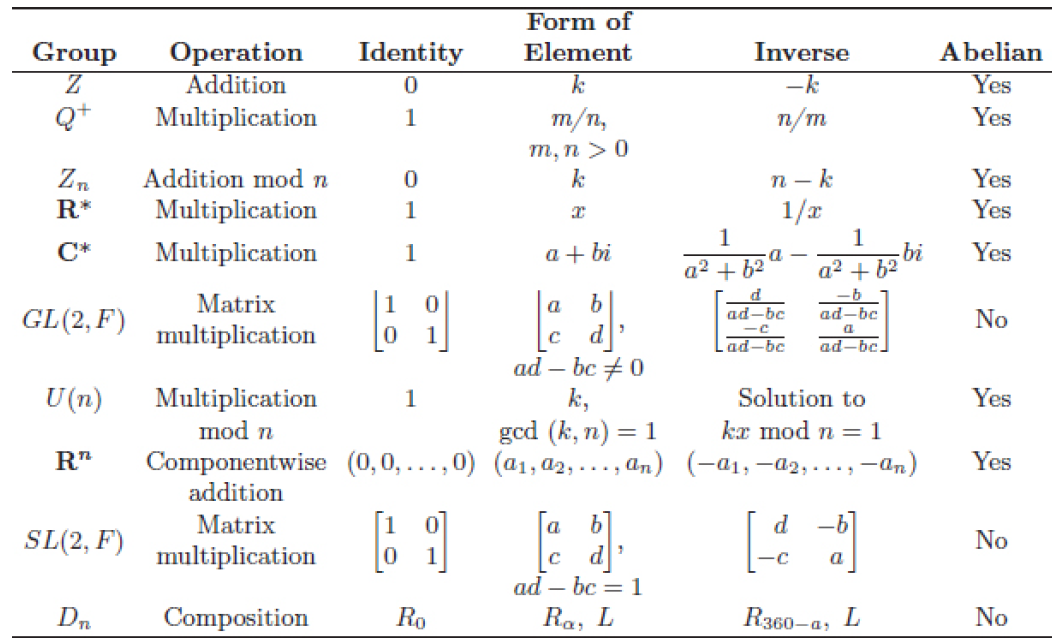
\includegraphics[width=\textwidth]{figures/group_example.png}
    \caption{Summary of Group Examples ($\mathbb{F}$ can be any of $\mathbb{Q,R,C}$, or $\mathbb{Z}_p$; $L$ is a reflection).} 
    \label{group_example}
\end{figure}

\subsection{Elementary Properties of Groups}
\fbox{\parbox{\linewidth}{
\begin{theorem}[Uniqueness of the Identity]
    Let $G$ be a group. Then
    \begin{equation*}
        e_1,e_2 \in G: \forall a \in G, ae_1=e_1a=a, ae_2=e_2a=a \implies e_1=e_2.
    \end{equation*}
\end{theorem}
}}

\begin{proof}
    Assume $G$ is a group and $\forall a \in G, \exists e_1,e_2 \in G: ae_1=e_1a = a, ae_2=e_2a=a$.
    \\ \\
    In particular, let $a=e_2$, then $e_2e_1 = e_1e_2 = e_2$. Let $a=e_1$, then $e_1e_2 = e_2e_1 = e_1$. It follows that $e_2e_1 = e_2$ and $e_2e_1 = e_1$. Hence $e_1=e_2$.
\end{proof}

\noindent\fbox{\parbox{\linewidth}{
\begin{theorem}[Cancellation]
    Let $G$ be a group. Then $\forall a,b,c \in G$,
    \begin{equation*}
         ba=ca \implies b=c \quad \text{and} \quad ab=ac \implies b=c.
    \end{equation*}
\end{theorem}
}}

\begin{proof}
    Let $G$ be a group. Then $\forall a \in G, \exists a^{-1} \in G: aa^{-1}=a^{-1}a=e$. If $ba = ca$, then by associativity,
    \begin{align*}
        ba &= ca \\
        (ba)a^{-1} &= (ca)a^{-1} \\
        b(aa^{-1}) &= c(aa^{-1}) \\
        be &= ce \\
        b &= c.
    \end{align*}
    If $ab = ac$, then by associativity,
    \begin{align*}
        ab &= ac \\
        a^{-1}(ab) &= a^{-1}(ac) \\
        (a^{-1}a)b &= (a^{-1}a)c \\
        eb &= ec \\
        b &= c.
    \end{align*}
\end{proof}

\noindent\fbox{\parbox{\linewidth}{
    \begin{theorem}[Uniqueness of Inverses]
        Let $G$ be a group. Then
        \begin{equation*}
            b_1,b_2 \in G: \forall a \in G, ab_1=b_1a=e, ab_2=b_2a=e \implies b_1=b_2.
        \end{equation*}
    \end{theorem}
}}

\begin{proof}
    Let $G$ be a group. Assume that $\forall a \in G, \exists b_1,b_2: ab_1=b_1a=e, ab_2=b_2a=e$. Then by associativity,
    \begin{align*}
        e = ab_1 &= ab_2 = e \\
        b_1(ab_1) &= b_1(ab_2) \\
        (b_1a)b_1 &= (b_1a)b_2 \\
        eb_1 &= eb_2 \\
        b_1 &= b_2.
    \end{align*}
\end{proof}

\begin{figure}[!htbp]
    \centering
    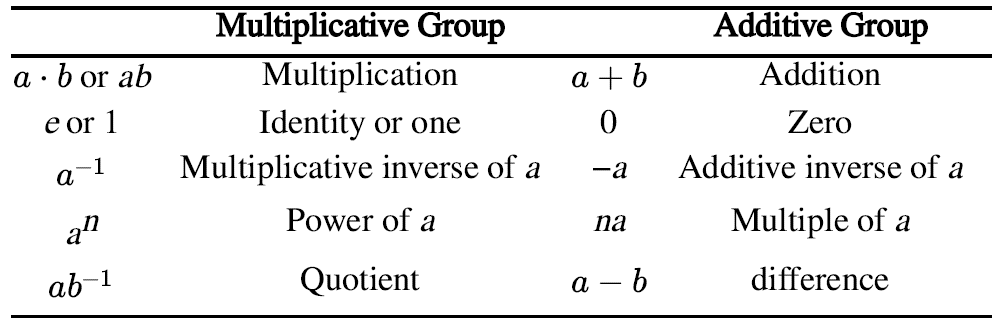
\includegraphics[width=0.8\linewidth]{figures/group_multi_add.png}
    \caption{}
    \label{group_multi_add}
\end{figure}

\noindent\fbox{\parbox{\linewidth}{
\begin{theorem}[Socks-Shoes Property]
    $G$ is a group $\implies \forall a,b \in G, (ab)^{-1} = b^{-1}a^{-1}$.
\end{theorem}
}}

\begin{proof}
    Let $G$ be a group and $a,b \in G$. So $ab, (ab)^{-1} \in G$. It follows that
    \begin{align*}
        (ab)(ab)^{-1} &= e, \\
        b(ab)^{-1} &= a^{-1}e, \\
        (ab)^{-1} &= b^{-1}a^{-1}e = b^{-1}a^{-1}.
    \end{align*}
\end{proof}

\section{Finite Groups; Subgroups}
\subsection{Terminology and Notation}
\fbox{\parbox{\linewidth}{
\begin{definition}
    The number of elements of a group (finite or infinite) is its \textit{order}, denoted as $|G|$.
\end{definition}
}}

\begin{note}
    The group $\mathbb{Z}$ has infinite order. The group $U(10)=\{1,3,7,9\}$ under multiplication modulo 10 has order 4.
\end{note}

\noindent\fbox{\parbox{\linewidth}{
\begin{definition}
    The order of $g \in G$, denoted by $|g|=n$, is the smallest $n \in \mathbb{N}: g^n = e$. If no such $n$ exists, then $|g|=\infty$. In additive notation, $\exists n \in \mathbb{N}: ng=0 \implies |g|=n$. 
\end{definition}
}}
\\ \\
\fbox{\parbox{\linewidth}{
\begin{definition}
    Let $G$ be a group. If $H \subseteq G$ is a group under the operation of $G$, then $H$ is a \textit{subgroup} of $G$, denoted $H \leq G$. If $H$ is a \textit{proper subgroup} of $G$, then $H < G$.
\end{definition}
}}

\begin{note}
   $H =\{e\}$ is the \textit{trivial} subgroup of $G$. $H \neq \{e\}$ is a \textit{nontrivial subgroup} of $G$.
   
   $\mathbb{Z}_n$ under addition modulo $n$ is not a subgroup of $\mathbb{Z}$ under addition, because addition modulo $n$ is not the operation of $\mathbb{Z}$.
\end{note}

\subsection{Subgroup Tests}
\fbox{\parbox{\linewidth}{
\begin{theorem}[One-Step Subgroup Test]
    Let $G$ be a group and $H \subseteq G, H \neq \emptyset$. Then
    \begin{equation*}
        a,b \in H, ab^{-1} \in H \implies H \leq G.
    \end{equation*}
    In additive notation, 
    \begin{equation*}
        a,b \in H, a-b \in H \implies H \leq G.
    \end{equation*}
\end{theorem}}}

\begin{proof}
    Let $G$ be a group and $H \subseteq G, H \neq \emptyset$. Assume that $a,b \in H, ab^{-1} \in H$. 
    \\ \\
    Since the operation of $H$ is the same operation in $G$, the operation is associative. Since $H \neq \emptyset \implies \exists x \in H$. Let $a=x,b=x$, then
    \begin{equation*}
        e = xx^{-1} = ab^{-1} \in H.
    \end{equation*}
    So $H$ has an identity $e$. Next, let $a=e,b=x$, then
    \begin{equation*}
        x^{-1} = ex^{-1} = ab^{-1} \in H.
    \end{equation*}
    So $x \in H \implies x^{-1} \in H$. Finally, since $y \in H \implies y^{-1} \in H$, let $a=x,b=y^{-1}$, then
    \begin{equation*}
        xy = x(y^{-1})^{-1} = ab^{-1} \in H.
    \end{equation*}
    So $x,y \in H \implies xy \in H$. Hence $H$ is a group under the operation in $G$ and by Definition 3.3, $H \leq G$.
    \end{proof}
    
    \begin{note}
       Although Theorem 3.1 is called One-Step Subgroup Test, there are actually four steps involved in applying the theorem:
    \begin{enumerate}
        \item Identify the property $P$ that distinguishes the elements of $H$. That is, identify a defining condition.
        \item Prove that the identity element has property $P$. This verifies $H \neq \emptyset$.
        \item Assume that $a,b$ have property $P$.
        \item Use the assumption that $a,b$ have property $P$ to show that $ab^{-1}$ has property $P$.
    \end{enumerate}
    \end{note}
    
    
    \begin{example}
    \begin{enumerate}
        \item Let $G$ be an Abelian group with identity $e$. Then $H = \{x \in G: x^2=e\}$ is a subgroup of $G$. The defining property of $H$ is the condition $x^2=e$. First, $e^2=e$, so $e \in H$ and $H \neq \emptyset$. Now assume that $a,b \in H,a^2=e,b^2=e$. Finally, since $G$ is Abelian,
        \begin{equation*}
            (ab^{-1})^2 = ab^{-1}ab^{-1} = aab^{-1}b^{-1} = a^2(b^2)^{-1} = ee^{-1} = e.
        \end{equation*}
        Hence $ab^{-1} \in H$ and by Theorem 3.1, $H \leq G$.
        
        \item Let $G$ be an Abelian group under multiplication with identity $e$. Then $H = \{x^2:x \in G\}$ is a subgroup of $G$. The defining property $P$ is that the elements have the form $x^2$. Since $e^2=e$, the identity has the correct form and $e \in H \implies H \neq \emptyset$. Next, write two elements in $H$ in the correct forms $a^2,b^2$. Since $G$ is Abelian,
        \begin{equation*}
            a^2(b^2)^{-1} = a^2(b^{-1})^2 = aab^{-1}b^{-1} = ab^{-1}ab^{-1} = (ab^{-1})^2,
        \end{equation*}
        which is the correct form. Hence $H \leq G$.
    \end{enumerate}
    \end{example}
    
    \noindent\fbox{\parbox{\linewidth}{
    \begin{theorem}[Two-Step Subgroup Test]
        Let $G$ be a group and $H \subseteq G, H \neq \emptyset$. If
        \begin{enumerate}[label=(\roman*)]
            \item $a,b \in H, ab \in H$ ($H$ is closed under the operation), and
            \item $a \in H, a^{-1}\in H$ ($H$ is closed under taking inverses),
        \end{enumerate}
        then $H \leq G$.
    \end{theorem}
    }}
    
    \begin{proof}
        Let $G$ be a group and $H \subseteq G, H \neq \emptyset$. Assume that $a,b \in H, ab \in H$ and $a \in H, a^{-1}\in H$. Then since the operation of $H$ is the same as the operation of $G$, the operation is associative in $H$. Next, let $a \in H$. Then $a^{-1} \in H, aa^{-1} \in H$ and
        \begin{equation*}
            e = aa^{-1} \in H.
        \end{equation*}
        Hence, $H$ is a group under the operation of $G$ and $H \leq G$.
    \end{proof}
    
    \begin{note}
       When applying Theorem 3.2, one proceeds exactly as in the case of Theorem 3.1, except one uses the assumption that $a,b$ have property $P$ to prove that $ab$ has property $P$ and that $a^{-1}$ has property $P$.
    \end{note}
    
    \begin{example}
    Let $G$ be an Abelian group. Then $H = \{x \in G: |x| \neq \infty\}$ is a subgroup of $G$. Since $e^1 = e$, it follows that $e$ has finite order so $e \in H$ and hence $H \neq \emptyset$. To apply Theorem 3.2, assume that $a,b \in H, |a|=m,|b|=n$. Then, since $G$ is Abelian,
    \begin{equation*}
        (ab)^{mn} = (a^m)^n(b^n)^m = e^ne^m = e.
    \end{equation*}
    Thus, $ab$ has finite order and $ab \in H$. This does not show that $|ab|=mn$, but $|ab| \leq mn$. Moreover, 
    \begin{equation*}
        (a^{-1})^m = (a^m)^{-1} = e^{-1} = e.
    \end{equation*}
    So $a^{-1}$ has finite order and $a^{-1} \in H$.
    \end{example}
    
    \begin{note}
       The next example illustrate how to use Theorem 3.2 by introducing an important technique for creating new subgroups of Abelian groups from existing ones.
    \end{note}
    
    \begin{example}
    Let $G$ be an Abelian group and $H,K \leq G$. Then $HK = \{hk: h \in H, k \in K\}$ is a subgroup of $G$. Since $e \in H, e \in K$, it follows that $e= ee \in HK$ and hence $HK \neq \emptyset$. Next, let $a,b \in HK$. Then by definition of $HK$
    \begin{equation*}
        \exists h_1,h_2 \in H, k_1,k_2 \in K: a=h_1k_1, b=h_2k_2.
    \end{equation*}
    Since $G$ is Abelian and $H,K \in G$, it follows that
    \begin{equation*}
        ab = (h_1k_1)(h_2k_2) = (h_1h_2)(k_2k_2) \in HK,
    \end{equation*}
    since $h_1h_2 \in H, k_1k_2 \in K$. Likewise,
    \begin{equation*}
        a^{-1} = (h_1k_1)^{-1} = k_1^{-1}h_1^{-1} = h_1^{-1}k_1^{-1} \in HK,
    \end{equation*}
    since $h_1^{-1} \in H, k_1^{-1} \in K$. Hence $HK \leq G$.
    \end{example}
    
    \begin{note}
       Any of the following ways guarantees that $H \subseteq G$ is not a subgroup of $G$.
    \begin{enumerate}
        \item Show that $e \notin H$.
        \item Show $\exists a \in H: a^{-1} \notin H$.
        \item Show $\exists a,b \in H: ab \notin H$.
    \end{enumerate}
    \end{note}
    
    \begin{example}
    Let $G$ be the group of nonzero real numbers under multiplication, let $H = \{x \in G: x=1 \vee x \in \mathbb{I}\}$ and $K= \{x \in G: x \geq 1\}$. Then $H \nleq G$, since $\sqrt{2} \in H$ but $\sqrt{2}\sqrt{2} \notin H$. Also, $K \nleq G$, since $2 \in K$ but $2^{-1} \notin K$.
    \end{example}
    
    \noindent\fbox{\parbox{\linewidth}{
    \begin{theorem}[Finite Subgroup Test]
        Let $H$ be a nonempty finite subset of a group $G$. Then $a,b \in H, ab \in H \implies$ $H \leq G$. 
    \end{theorem}
    }}
    
    \begin{proof}
        Let $G$ be a group, and let $H \subseteq G$,  $H$ is nonempty and finite. Assume that $a,b \in H, ab \in H$.
        \\ \\
        If $a=e$, then 
        \begin{equation*}
            a^{-1} = e^{-1} = e = a \in H.
        \end{equation*}
        Since $a,b \in H, ab \in H, a^{-1} \in H$, by Theorem 3.2, $H \leq G$. 
        \\ \\
        If $a \neq e$, consider the sequence $a, a^2, \dots$. Since $a,b \in H,ab \in H$, it follows that
        \begin{align*}
            a &\in H \\
            a^2 = aa &\in H \\
            a^3 = aa^2 &\in H \\
            &\vdots
        \end{align*}
        and hence $a,a^2,\dots \in H$. Since $H$ is finite, not all of these elements are distinct. Assume $a^i=a^j, i> j$. Then 
        \begin{align*}
            a^i &= a^j \\
            a^ia^{-j} &= a^ja^{-j} \\
            a^{i-j} &= e.
        \end{align*}
        Since $a \neq e$, it follows that $i-j>1$. Thus
        \begin{equation*}
            aa^{i-j-1} = a^{i-j} = e
        \end{equation*}
        and hence $a^{i-j-1}=a^{-1}$. But $i-j>1 \implies i-j-1 >0 \implies a^{i-j-1} \in H$. So $a,b \in H, ab \in H, a^{-1} \in H$ and by Theorem 3.2, $H \leq G$.
    \end{proof}
    
    \subsection{Examples of Subgroups}
    \fbox{\parbox{\linewidth}{
        \begin{definition}
            $\forall a \in G, \langle a \rangle = \{a^n: n \in \mathbb{Z}\} = \{\dots,a^{-2},a^{-1},a^0=e,a^1,a^2,\dots\}$.
        \end{definition}
    }}
    \\ \\
    \fbox{\parbox{\linewidth}{
    \begin{theorem}[$\langle a \rangle$ is a Subgroup]
        Let $G$ be a group, and let $a \in G$. Then, $\langle a \rangle \leq G$.
    \end{theorem}
    }}
    
    \begin{proof}
        Let $G$ be a group and $a \in G$. Since $a \in \langle a \rangle$, it follows that $\langle a \rangle \neq \emptyset$. Let $a^n,a^m \in \langle a \rangle$. Then, $a^n(a^m)^{-1} = a^{n-m} \in \langle a \rangle$. Hence by Theorem 3.1, $\langle a \rangle \leq G$.
    \end{proof}
    
    $\langle a \rangle$ is the \textit{cyclic subgroup 5 of $G$ generated by $a$}. If $G = \langle a \rangle$, then $G$ is \textit{cyclic} and $a$ is a generator of $G$. A cyclic group may have many generators. Although the list $\dots,a^{-2},a^{-1},a^0,a^1,a^2,\dots$ has infinitely many entries, the set $\{a^n: n \in \mathbb{Z}\}$ might have only finitely many elements. Also, since $a^ia^j=a^{i+j}=a^{j+i}=a^ja^i$, every cyclic group is Abelian.
    
    \begin{example}
    \begin{enumerate}
        \item For $U(10)=\{1,3,7,9\}$ under multiplication modulo 10, since
        \begin{equation*}
            3^0=1, 3^1 = 3, 3^2 = 9, 3^3 = 7, 3^4 =1, 3^5=3^4\cdot3^1=1\cdot3=3, \dots.
        \end{equation*}
        and since $3\cdot7=1$ and 1 is the identity, it follows that $3^{-1}=7$. So
        \begin{equation*}
            3^{-1}=7, 3^{-2}=3^{-1}3^{-1}=7\cdot7=9, 3^{-3}=3^{-2}3^{-1}=9\cdot7=3, \dots.
        \end{equation*}
        Hence $\langle 3 \rangle = \{3,9,7,1\} = U(10)$ under multiplication modulo 10.
        
        \item For $\mathbb{Z}_{10}$ under addition modulo 10, since 
        \begin{equation*}
            0(2)=0, 1(2)=2, 2(2)=4, 3(2)=6, 4(2)=8, 5(2)=0, 6(2)=2, \dots
        \end{equation*}
        and since $-2=10(-1)+8$, it follows that
        \begin{equation*}
            -1(2)=8, -2(2)=-4=6, -3(2)=-6=4, -4(2)=-8=2, \dots.
        \end{equation*}
        Hence, $\langle 2 \rangle = \{2,4,6,8,0\}$ and since $a,b \in \langle 2 \rangle \implies ab \in \langle 2 \rangle$. For instance,
        \begin{equation*}
            0\cdot2  = 0, 2\cdot4 = 8, 8\cdot8 = 4, \dots \in \langle 2 \rangle.
        \end{equation*}
        Hence by Theorem 3.3, $\langle 2 \rangle = \{2,4,6,8,0\} \leq \mathbb{Z}_{10}$.
        
        \item For $\mathbb{Z}$, since
        \begin{align*}
            \langle -1 \rangle &= \{\dots,-2(-1),-1(-1),0(-1),1(-1),2(-1),\dots\} \\
            &= \{\dots, -2,-1,0,1,2,\dots\} = \mathbb{Z}.
        \end{align*}
        Hence $\langle -1 \rangle = \mathbb{Z}$.
        \item
        \item
    \end{enumerate}
    \end{example}
    
    For any $a \in G$, it is useful to think of $\langle a \rangle$ as the smallest subgroup of $G$ containing $a$. This notion can be extended to any collection $S$ of elements from $G$ by defining $\langle S \rangle$ as the subgroup of $G$ with the property that $S \in \langle S \rangle$ and if $H$ is any subgroup of $G$ containing $S$, then $H$ also contains $\langle S \rangle$. Thus $\langle S \rangle$ is the smallest subgroup of $G$ that contains $S$. $\langle S \rangle$ is \textit{the subgroup generated by $S$}.
    
    \begin{example}
    In $\mathbb{Z}_{20},\langle 8,14 \rangle = \{0,2,4,\dots,18\}=\langle 2 \rangle$. 
    \\ \\
    In $\mathbb{Z}, \langle 8,13 \rangle = \mathbb{Z}$.
    \\ \\
    In $D_4, \langle H,V \rangle = \{H,H^2,V,HV\} = \{R_0,R_{180},H,V\}$.
    \\ \\
    In $D_4, \langle R_{9},V\rangle = \{R_{90},R_{90}^2,R_{90}^3,R_{90}^4,V,R_{90}V,R_{90}^2V,R_{90}^3V\}=D_4$.
    \end{example}
    
    \noindent\fbox{\parbox{\linewidth}{
    \begin{definition}
        The center of a group $G$ is
        \begin{equation*}
            Z(G) = \{a \in G: \forall x \in G, ax=xa\}.
        \end{equation*}
    \end{definition}
    }}
    \\ \\
    \fbox{\parbox{\linewidth}{
    \begin{theorem}[Z(G) is a Subgroup]
        Let $G$ be a group and $Z(G)$ be the center of $G$. Then $Z(G) \leq G$.
    \end{theorem}
    }}
    
    \begin{proof}
        Let $G$ be a group and $Z(G)$ be the center of $G$. Since $\forall x \in G, ex = xe$, it follows that $e \in Z(G)$ and hence $Z(G) \neq \emptyset$. Assume that $a,b \in Z(G)$, then since the operation of $G$ is associative,
        \begin{equation*}
            \forall x \in G, (ab)x = a(bx) = a(xb) = (ax)b = (xa)b = x(ab).
        \end{equation*}
        Hence $ab \in Z(G)$.
        
        Next, assume that $a \in Z(G)$. Then $\forall x \in G, ax = xa$ and
        \begin{align*}
            ax &= xa, \\
            a^{-1}(ax)a^{-1} &= a^{-1}(xa)a^{-1}, \\
            (a^{-1}a)xa^{-1} &= a^{-1}x(aa^{-1}), \\
            exa^{-1} &= a^{-1}xe, \\
            xa^{-1} &= a^{-1}x.
        \end{align*}
        Hence $a^{-1} \in Z(G)$ and by Theorem 3.2, $Z(G) \leq G$.
    \end{proof}
    
    \begin{example}
        Let $n \geq 3$. Observe that since $R \in D_n, R = (R_{360/n})^k, k \in \mathbb{Z}$, so $R,R' \in D_n, RR'=R'R$. Let $R \in D_n$ be any rotation and let $F \in D_n$ be any reflection. Since $RF$ is a reflection, it follows that
        \begin{equation*}
            RF = (RF)^{-1} = F^{-1}R^{-1} = FR^{-1}.
        \end{equation*}
        Thus
        \begin{equation*}
            RF = FR \iff FR = RF = FR^{-1}.
        \end{equation*}
        By cancellation, $R = R^{-1}$. But $R = R^{-1}$ only when $R=R_0$ or $R=R_{180}$ and $R_{180}$ is in $D_n$ only when $n$ is even. So,
        \begin{equation*}
            Z(D_n) = \bigg\{ \begin{matrix}
               \{R_0,R_{180}\} & ,n \text{ is even,} \\
               \{R_0\} & ,n \text{ is odd.}
            \end{matrix}
        \end{equation*}
    \end{example}
    
    \noindent\fbox{\parbox{\linewidth}{
    \begin{definition}
        Let $a$ be a fixed element of a group $G$. The \textit{centralizer} of $a$ in $G$ is
        \begin{equation*}
            C(a) = \{g \in G: ga = ag\}.
        \end{equation*}
    \end{definition}
    }}
    
    \noindent\fbox{\parbox{\linewidth}{
    \begin{theorem}[C(a) is a Subgroup]
        Let $G$ be a group. Then
        \begin{equation*}
            \forall a \in G, C(a) \leq G.
        \end{equation*}
    \end{theorem}
    }}
    
    \begin{proof}
        Let $G$ be a group, $a \in G$ be arbitrary, and $C(a)$ be a centralizer of $a$ in $G$. Since $e \in G, ea=ae$, it follows that $e \in C(a)$ and hence $C(a) \neq \emptyset$. Assume that $x,y \in C(a)$. Then, since the operation in $G$ is associative,
        \begin{equation*}
            (xy)a = x(ya) = x(ay) = (xa)y = (ax)y = a(xy).
        \end{equation*}
        Hence $xy \in C(a)$.
        \\ \\
        Next, assume that $x \in C(a)$. Then $xa = ax$ and
        \begin{align*}
            xa &= ax, \\
            x^{-1}(xa)x^{-1} &= x^{-1}(ax)x^{-1}, \\
            (x^{-1}x)ax^{-1} &= x^{-1}a(xx^{-1}), \\
            eax^{-1} &= x^{-1}ae, \\
            ax^{-1} &= x^{-1}a.
        \end{align*}
        Hence $x^{-1} \in C(a)$ and by Theorem 3.2, $C(a) \leq G$.
    \end{proof}
    
    Note that $\forall a \in G, Z(G) \subseteq C(a)$. Also, $G$ is Abelian iff $\forall a \in G, C(a) = G$.
    
    \begin{example}
        In $D_4$,
        \begin{align*}
            C(R_0) &= D_4 = C(R_{180}), \\
            C(R_{90}) &= \{R_0, R_{90}, R_{180}, R_{270}\} = C(R_{270}), \\
            C(H) &= \{R_0, H, R_{180}, V\} = C(V), \\
            C(D) &= \{R_0, D, R_{180}, D'\} = C(D').
        \end{align*}
    \end{example}
    
\section{Cyclic Groups}
\subsection{Properties of Cyclic Groups}
\fbox{\parbox{\linewidth}{
\begin{definition}
    Let $G$ be a group. Then
    \begin{equation*}
        \exists a \in G: G = \langle a \rangle = \{a^n: n \in \mathbb{Z}\} \implies G \text{ is cyclic.}
    \end{equation*}
    $a \in G$ is a generator of $G$.
\end{definition}
}}

\begin{example}
    \begin{enumerate}
        \item $\mathbb{Z}$ under addition is cyclic. Since
        \begin{align*}
            \langle 1 \rangle &= \{n1: n \in \mathbb{Z}\} \\
            &=  \{\dots, -2(1), -1(1), 0(1), 1(1), 2(1), \dots\} \\
            &= \{\dots, -2, -1, 0, 1, 2, \dots\} \\
            &= \mathbb{Z}
        \end{align*}
        and
        \begin{align*}
            \langle -1 \rangle &= \{n(-1): n \in \mathbb{Z}\} \\
            &=  \{\dots, 2(-1), 1(-1), 0(-1), -1(-1), -2(-1), \dots\} \\
            &= \{\dots, -2, -1, 0, 1, 2, \dots\} \\
            &= \mathbb{Z}.
        \end{align*}
        Hence $\mathbb{Z} = \langle 1 \rangle = \langle -1 \rangle$ and $-1,1$ are the generators of $\mathbb{Z}$.
        
        \item $\mathbb{Z}_n = \{0,1,\dots,n-1\}, n \geq 1$ under addition modulo $n$ is a cyclic group. Since
        \begin{align*}
            1(1) &= 1, & 0(1) &= 0, \\ 
            2(1) &= 2, & -1(1) &= -1 =n-1, \\ 
            & \vdots  & \vdots \\ 
            (n-1)(1) &= n-1, & -(n-1)(1) &= 1, \\ 
            n(1) &= 0, & -n(1)  &= -n = 0, \\ 
            & \vdots & \vdots
        \end{align*}
        and
        \begin{align*}
            1(-1) &= -1=n-1, & 0(-1) &= 0, \\
            2(-1) &= -2=n-2, & -1(-1) &= 1, \\
            & \vdots & \vdots \\
            (n-1)(1) &= n-1, & -(n-1)(-1) &= n-1, \\
            &\vdots & \vdots
        \end{align*}
        it follows that $\mathbb{Z}_n=\langle 1 \rangle = \langle -1 \rangle$. Hence $1,-1=n-1$ are the generators of $\mathbb{Z}_n$.
        
        \item For $\mathbb{Z}_8$ under addition modulo 8. Since
        \begin{align*}
            \langle 1 \rangle = \{1,2,3,4,5,6,7,0\}, \\
            \langle 3 \rangle = \{3,6,1,4,7,2,5,0\}, \\
            \langle 5 \rangle = \{5,2,7,4,1,6,3,0\}, \\
            \langle 7 \rangle = \{7,6,5,4,3,2,1,0\},
        \end{align*}
        it follows that $\mathbb{Z}_8 = \langle 1 \rangle = \langle 3 \rangle = \langle 5 \rangle = \langle 7 \rangle$. Hence $1,3,5,7$ are the generators of $\mathbb{Z}_8$. On the other hand, 2 is not a generator since $\langle 2 \rangle = \{2,4,6,0\} \neq \mathbb{Z}_8$.
        
        \item For $U(10)=\{1,3,7,9\}$, since $\langle 3 \rangle = \{3,9,7,1\}, \langle 7 \rangle = \{7,9,3,1\}$, it follows that $U(10)=\langle 3 \rangle = \langle 7 \rangle$. Hence $3,7$ are generators of $U(10)$.
        
        \item For $U(8)=\{1,3,5,7\}$, since $\langle 1 \rangle = \{1\}, \langle 3 \rangle = \{3,1\}, \langle 5 \rangle = \{5,1\}, \langle 7 \rangle = \{7, 1\}$, it follows that $U(8) \neq \langle a \rangle, a \in U(8)$. Hence $U(8)$ is not cyclic.
    \end{enumerate}
\end{example}

\noindent\fbox{\parbox{\linewidth}{
\begin{theorem}
    Let $G$ be a group and $a \in G$. 
    \begin{enumerate}[label=(\roman*)]
        \item $|a|=\infty \implies (a^i=a^j \iff i=j)$.
                
        \item $|a|=n \implies \langle a \rangle = \{e,a,a^2,\dots,a^{n-1}\}$ and $a^i=a^j \iff n \mid (i-j)$.
    \end{enumerate}
\end{theorem}
}}

\begin{proof}
    Let $G$ be a group and $a \in G$.
    \\ \\
    (i) Assume that $|a|=\infty$. Then $a^n \neq e, n \in\mathbb{N}$. 
    \\ \\
    $(\Rightarrow)$ Assume that $a^i = a^j$. Then $a^{i-j}=e$, it follows that $i-j=0 \implies i=j$.
    \\ \\
    $(\Leftarrow)$ Assume that $i=j$. Then $i-j=0$ and hence $a^{i-j}=a^0=e \implies a^i = a^j$.
    \\ \\
    Hence, $|a|=\infty \implies (a^i=a^j \iff i=j)$.
    \\ \\
    (ii) Assume that $|a|=n$, so $a^n = e$. Let $a^k \in \langle a \rangle$ be arbitrary. By the division algorithm,
    \begin{equation*}
        \exists q,r \in \mathbb{Z}: k=nq+r, 0\leq r <n.
    \end{equation*}
    So
    \begin{equation*}
        a^k = a^{nq+r} = a^{nq}a^r = (a^n)^qa^r = e^qa^r = ea^r = a^r.
    \end{equation*}
    Since $0 \leq r<n$, it follows that $e \leq a^k < a^n$ and
    $a^k \in \{e,a,a^2,\dots,a^{n-1}\}$. Hence, $\langle a \rangle \subseteq \{e,a,a^2,\dots,a^{n-1}\}$.
    \\ \\
    Let $a^k \in \{e,a,\dots,a^{n-1}\}$. Then $a^k \in \langle a \rangle = \{a^t: t \in \mathbb{Z}\}$ and $\{e,a,\dots,a^{n-1}\} \subseteq \langle a \rangle$. Hence $\langle a \rangle = \{e,a,\dots,a^{n-1}\}$.
    \\ \\
    $(\Rightarrow)$ Assume that $a^i=a^j$, so $a^{i-j}=e$. By the division algorithm, 
    \begin{equation*}
        \exists q,r \in \mathbb{Z}: i-j=nq+r, 0\leq r <n.
    \end{equation*}
    So
    \begin{equation*}
        e = a^{i-j} = a^{nq+r} = a^{nq}a^r = (a^n)^qa^r = e^qa^r = ea^r = a^r.
    \end{equation*}
    Since $n$ is the smallest positive integer s.t. $a^n=e$, it follows that $r=0$ and $i-j = nq \implies n \mid (i-j)$.
    \\ \\
    $(\Leftarrow)$ Assume that $n \mid (i-j)$, so $i-j=nq$. It follows that
    \begin{equation*}
        a^{i-j} = a^{nq} = (a^n)^q = e^q = e
    \end{equation*}
    and hence $a^i=a^j$.
    \\ \\
    Hence $|a|=n \implies \langle a \rangle = \{e,a,a^2,\dots,a^{n-1}\}$ and $a^i=a^j \iff n \mid (i-j)$.
\end{proof}

\noindent\fbox{\parbox{\linewidth}{
\begin{corollary}
    Let $G$ be a group. Then $\forall a \in G, |a|=|\langle a \rangle|$.
\end{corollary}
}}

\begin{proof}
   Let $G$ be a group, let $a \in G$ be arbitrary. Assume that $|a|=n$, then $\langle a \rangle = \{e,a,\dots,a^{n-1}\}$. It follows that $|\langle a \rangle| = n$.
\end{proof}

\noindent\fbox{\parbox{\linewidth}{
\begin{corollary}
    Let $G$ be a group. Then $\forall a \in G, a^k=e \iff |a| \mid k$.
\end{corollary}
}}

\begin{proof}
    From Theorem 4.1 (ii), $a^k = e = a^0 \iff (n = |a|) \mid (k-0=k)$.
\end{proof}

\noindent\fbox{\parbox{\linewidth}{
\begin{corollary}
     Let $G$ be a group. Then $\forall a \in G, a^k=e \iff k$ is a multiple of $|a|$.
\end{corollary}
}}
\\ \\
\fbox{\parbox{\linewidth}{
\begin{corollary}
     Let $G$ be a finite group. Then
     \begin{equation*}
         a,b \in G, ab=ba \implies |ab| \mid |a||b|.
     \end{equation*}
\end{corollary}
}}

\begin{proof}
    Let $|a|=m,|b|=n$. Then
    \begin{equation*}
        (ab)^{mn} = (a^m)^n(b^n)^m = e^ne^m = e.
    \end{equation*}
    Hence by Corollary 4.1.2, $|a| \mid mn = |a||b|$.
\end{proof}

Figure \ref{thm4.1} shows Theorem 4.1 and its corollaries for $|a|=6$.

\begin{figure}[!htbp]
    \centering
    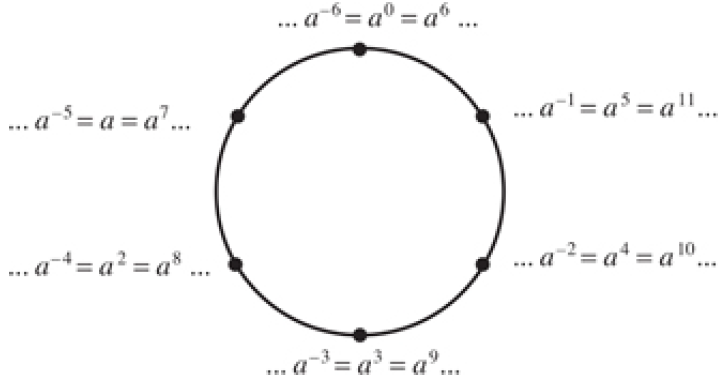
\includegraphics[width=0.6\linewidth]{figures/thm4.1.png}
    \caption{Powers of $a$ for $|a|=6$.}
    \label{thm4.1}
\end{figure}

\noindent\fbox{\parbox{\linewidth}{
\begin{theorem}
    Let $G$ be a group, $a \in G, |a|=n$, and let $k \in \mathbb{N}$. Then 
    \begin{enumerate}[label=(\roman*)]
        \item $\langle a^k \rangle = \langle a^{\gcd (n,k)} \rangle$ and 
        \item $|a^k| = n/\gcd (n,k)$.
    \end{enumerate}
\end{theorem}
}}

\begin{proof}
    Let $G$ be a group, $a \in G, |a|=n$, and let $k \in \mathbb{N}$.
    \\ \\
    (i) Let $d=\gcd (n,k)$ and let $k=dr$. Since $a^k=(a^d)^r \in \langle a^d \rangle$, it follows that $\langle a^k \rangle \subseteq \langle a^d \rangle$. By Theorem 0.2, $\exists s,t \in \mathbb{Z}: d = ns+kt$. So
    \begin{equation*}
        a^d = a^{ns+kt} = a^{ns}a^{kt} = (a^n)^s(a^k)^t = e(a^k)^t = (a^k)^t \in \langle a^k \rangle.
    \end{equation*}
    Hence, $\langle a^d \rangle \subseteq \langle a^k \rangle$ and $\langle a^k \rangle = \langle a^{\gcd (n,k)} \rangle$.
    \\ \\
    (ii) Let $d$ be any divisor of $n$. Then $(a^d)^{n/d} = a^n = e \implies |a^d| \leq n/d$. Let $i \in \mathbb{N}, i < n/d$. If $(a^d)^i=a^{di}=e$, then since $|a|=n$, it follows that $di \geq n \implies i \geq n/d$, contradicting that $i<n/d$. Hence $|a^d|=n/d$. Now let $d = \gcd (n,k)$, then
    \begin{align*}
        |a^k| &= |\langle a^k \rangle| \quad \text{(by Corollary 4.1.1)} \\
        &= |\langle a^{\gcd (n,k)} \rangle| \quad \text{(by part (i))} \\
        &= |a^{\gcd (n,k)}| \\
        &= |a^d| \\
        &= n/d \\
        &= n/\gcd (n,k).
    \end{align*}
\end{proof}

\begin{example}
    \begin{enumerate}
        \item For $|a|=30$, find $\langle a^{26} \rangle, \langle a^{17} \rangle, \langle a^{18} \rangle, |a^{26}|, |a^{17}|, |a^{18}|$.
        \\ \\
        Since $\gcd(30,26)=2$, by Theorem 4.2 (i), $\langle a^{26} \rangle = \langle a^{\gcd(30,26)} \rangle = \langle a^2 \rangle$.
        Since
        \begin{align*}
            (a^2)^1 &= a^2, (a^2)^2=a^4, \dots, (a^2)^{14}=a^{28}, (a^2)^{15}=a^{30}=e, \\ (a^2)^{16} &= a^{32}=a^{30}a^{2}=ea^{2}=a^{2}, (a^2)^{17} = a^{34}=a^{30}a^{4}=ea^{4}=a^{4}, \dots
        \end{align*}
        and
        \begin{align*}
            (a^2)^0 &= e, \\
            (a^2)^{-1} &= (a^2)^{-1}\cdot e = (a^2)^{-1}a^{30} = (a^2)^{-1}(a^2)^{15} = (a^2)^14 = a^{28}, \\
            (a^2)^{-2} &= (a^2)^{-1}(a^2)^{-1} = a^{28}a^{28} = a^{56} = a^{30}a^{26} = a^{26}, \\
            & \vdots
        \end{align*}
        it follows that $\langle a^{26} \rangle = \langle a^2 \rangle = \{e,a^2,a^4,\dots,a^{26},a^{28}\}$ and $|a^{26}|=30/\gcd(30,26)=30/2=15$.
        \\ \\
        Since $\gcd(30,17)=1$, it follows that $\langle a^{17} \rangle = \langle a^1 \rangle = \{e,a,a^2,\dots,a^{29}\}$ and $|a^{17}|=30/1=30$.
        \\ \\
        Since $\gcd(30,18)=6$, it follows that $\langle a^{18} \rangle = \langle a^6 \rangle$. Since
        \begin{equation*}
            (a^6)^1=a^6, (a^6)^2=a^{12}, (a^6)^3=a^{18}, (a^6)^4=a^{24}, (a^6)^5=a^{30}=e, \dots
        \end{equation*}
        and
        \begin{align*}
            (a^6)^0=e, (a^6)^{-1} = (a^6)^{-1}a^{30} = (a^6)^{-1}(a^6)^5 = (a^6)^4 = a^{24}, \dots,
        \end{align*}
        it follows that $\langle a^18 \rangle = \langle a^6 \rangle = \{e,a^6,a^{12},a^{18},a^{24}\}$ and $|a^{18}|=30/\gcd(30,18)=30/6=5$.
        
        \item For $|a|=1000$, find $\langle a^{140} \rangle, \langle a^{400} \rangle, \langle a^{62} \rangle, |a^{140}|, |a^{400}|, |a^{62}|$.
        \\ \\
        Since $\gcd(1000,140) = \gcd(2^35^3,2^25\cdot7) = 2^25 = 20$, it follows that $\langle a^{140} \rangle = \langle a^{20} \rangle = \{e,a^{20},a^{40},a^{60},\dots,a^{980}\}$ and $|a^{140}|=1000/20=50$.
        \\ \\
        Since $\gcd(1000,400) = \gcd(2^35^3,2^45^2)=2^35^2=200$, it follows that $\langle a^{400} \rangle= \langle a^{200} \rangle = \{e,a^{200},a^{400},a^{600},a^{800}\}$ and $|a^{140}|=1000/200=5$.
        \\ \\
        Since $\gcd(1000,62) = \gcd(2^35^3,2\cdot31)=2$, it follows that $\langle a^{62} \rangle = \langle a^{2} \rangle = \{e,a^2,a^4,a^6,a^{998}\}$ and $|a^{62}|=1000/2=500$.
        \\
    \end{enumerate}
    
    \noindent\fbox{\parbox{\linewidth}{
    \begin{corollary}
         $G = \langle a \rangle, |G| = n \implies \forall g \in G, |g| \mid |G|$. 
    \end{corollary}
    }}
    \begin{proof}
        Let $G = \langle a \rangle, a \in G$ and $|G| = |\langle a \rangle| = |a| = n$. Let $g \in G$ be arbitrary, since $G = \langle a \rangle$, it follows that $g = a^k$. By Theorem 4.2 (ii),
        \begin{equation*}
            |g| = |a^k| = n / \gcd(n,k) = |G| / \gcd(n,k).
        \end{equation*}
        Hence, $|a| \mid G, a \in G$.
    \end{proof}
    
    \noindent\fbox{\parbox{\linewidth}{
    \begin{corollary}
         Let $|a|=n$. Then
         \begin{enumerate}[label=(\roman*)]
             \item $\langle a^i \rangle = \langle a^j \rangle \iff \gcd(n,i)=\gcd(n,j)$, and
             \item $|a^i|=|a^j| \iff \gcd(n,i)=\gcd(n,j)$.
         \end{enumerate}
    \end{corollary}
    }}
    \begin{proof}
        Let $|a|=n$.
        \\ \\
        (i) $(\Rightarrow)$ Assume that $\langle a^i \rangle = \langle a^j \rangle$. By Theorem 4.2 (i),
        \begin{align*}
            \langle a^i \rangle = \langle a^j \rangle \implies \langle a^{\gcd(n,i)} \rangle = \langle a^{\gcd(n,j)} \rangle,
        \end{align*}
        which implies that $|a^{\gcd(n,i)}| = |a^{\gcd(n,j)}|$ since two sets are equal if they have the same members. By Theorem 4.2 (ii),
        \begin{equation*}
            |a^{\gcd(n,i)}| = |a^{\gcd(n,j)}| \implies n/\gcd(n,i) = n/\gcd(n,j) \implies \gcd(n,i)=\gcd(n,j).
        \end{equation*}
        
        $(\Leftarrow)$ Assume that $\gcd(n,i)=\gcd(n,j)$. Then it follows that $\langle a^i \rangle = \langle a^j \rangle$.
        \\ \\
        (ii) $(\Rightarrow)$ Assume that $|a^i|=|a^j|$. Then by Theorem 4.2 (ii),
        \begin{align*}
            |a^i| &= |a^j|, \\
            n/\gcd(n,i) &= n/\gcd(n,j), \\
            \gcd(n,i) &= \gcd(n,j).
        \end{align*}
        
        $(\Leftarrow)$ Assume that $\gcd(n,i) = \gcd(n,j)$. Then
        \begin{align*}
            \gcd(n,i) &= \gcd(n,j), \\
            n \cdot \gcd(n,i) &= n \cdot \gcd(n,j), \\
            n/\gcd(n,i) &= n/\gcd(n,j), \\
            |a^i| &= |a^j| \quad \text{(by Theorem 4.2 (ii))}.
        \end{align*}
    \end{proof}
    
    \noindent\fbox{\parbox{\linewidth}{
    \begin{corollary}
         Let $|a|=n$. Then
        \begin{enumerate}[label=(\roman*)]
            \item $\langle a \rangle = \langle a^j \rangle \iff \gcd(n,j)=1$, and
            \item $|a|=|a^j| \iff \gcd(n,j)=1$.
        \end{enumerate}
    \end{corollary}
    }}
    
    \begin{example}
        For $U(50) = \{1,3,7,9,11,13,17,19,\dots,47,49\}, |U(50)|=20$. Since
        \begin{align*}
            3^1 \bmod{50} &= 3, 3^2\bmod50=9, 3^3\bmod50=27, 3^4\bmod50=31, \dots, \\
            3^0\bmod50 &= 1, 3^{-1}\bmod50=3^{19}\bmod50=17, \dots,
        \end{align*}
        it follows that $U(50)=\langle3\rangle$ and 3 is a generator of $U(50)$. By Corollary 4.2.3, $\gcd(50,3)=1 \iff \langle3\rangle = \langle3^3\rangle$, so $U(50)=\langle3\rangle=\langle3^3\rangle=\langle27\rangle$ and 27 is a generator of $U(50)$. The complete list of generators of $U(50)$ is
        \begin{align*}
            3^1\bmod50 &= 3, 3^3\bmod50=27, 3^7\bmod50=37, 3^9\bmod50=33, \\ 
            3^{11}\bmod50 &= 47, 3^{13}\bmod50=23, 3^{17}\bmod50=13, 3^{19}\bmod50=17.
        \end{align*}
    \end{example}
    
    \noindent\fbox{\parbox{\linewidth}{
    \begin{corollary}
         $k \in \mathbb{Z}_n$ is a generator of $\mathbb{Z}_n$ $\iff \gcd(n,k)=1$.
    \end{corollary}
    }}
\end{example}

\subsection{Classification of Subgroups of Cyclic Groups}
\fbox{\parbox{\linewidth}{
\begin{theorem}[Fundamental Theorem of Cyclic Groups]
    Let $G$ be cyclic. Then 
    \begin{equation*}
        H \leq G \implies H \text{ is cyclic.}
    \end{equation*}
     Moreover, if $|\langle a\rangle|=n$, then
        \begin{enumerate}
            \item $H \leq \langle a \rangle \implies |H|\mid n$.
            \item $k \mid n, k>0, !\exists H \leq \langle a \rangle: |H|=k, H = \langle a^{n/k} \rangle$.
        \end{enumerate}
\end{theorem}
}}
\begin{proof}
    Let $G$ be a cyclic group, so $\exists a \in G$: $G=\langle a \rangle$.
    \\ \\
    (i) Assume that $H \leq G = \langle a \rangle$. If $H=\{e\}$, then $H$ is cyclic. If $H \neq \{e\}$, then
    \begin{equation*}
        H \leq G = \langle a \rangle \implies \forall x \in H, x = a^t, t \in \mathbb{Z}.
    \end{equation*}
    If $a^t \in H, t<0$, then
    \begin{equation*}
        H \leq G \implies a^{-t} \in H, -t>0.
    \end{equation*}
    Hence $\exists a^t \in H, t > 0$. Let $m = \min\{t \in\mathbb{N}:a^t \in H\}$. Then by closure, $(a^m)^t \in H, t \in \mathbb{Z}$. Hence $\langle a^m \rangle \subseteq H$.
    
    Let $b \in H$ be arbitrary. Then
    \begin{equation*}
        H \leq G = \langle a \rangle \implies b = a^k, k \in \mathbb{Z}.
    \end{equation*}
    By the division algorithm,
    \begin{equation*}
        \exists q,r \in \mathbb{Z}: k=mq+r, 0 \leq r < m.
    \end{equation*}
    So
    \begin{equation*}
        a^k = a^{mq+r} = a^{mq}a^r
    \end{equation*}
    and
    \begin{equation*}
        a^r = a^{-mq}a^k = (a^m)^{-q}a^k.
    \end{equation*}
    By closure,
    \begin{equation*}
        (a^m)^{-q},a^k \in H \implies a^{-mq}a^k=a^r \in H.
    \end{equation*}
    But 
    \begin{equation*}
        a^m \in H, m = \min\{t \in\mathbb{N}:a^t \in H\}, 0 \leq r < m \implies r=0,
    \end{equation*}
    so
    \begin{equation*}
        k = mq+r=mq \quad \text{and} \quad a^k = a^{mq}a^r = a^{mq} = (a^m)^q.
    \end{equation*}
    Hence,
    \begin{equation*}
        a^k \in \langle a^m \rangle \implies H \subseteq \langle a^m \rangle
    \end{equation*}
    and
    \begin{equation*}
        \langle a^m \rangle \subseteq H, H \subseteq \langle a^m \rangle \implies H = \langle a^m \rangle. \\
    \end{equation*}
    
    \noindent(ii) Let $|G|=|\langle a \rangle|=n$. Then
    \\ \\
    (a) Assume that $H \leq G = \langle a \rangle$. Then by Theorem 4.3 (i), $H = \langle a^m \rangle$ and $a^k \in H = \langle a^m \rangle \implies k = mq, q \in \mathbb{Z}$. Since
    \begin{equation*}
        |G| = |\langle a \rangle| = |a| = n \implies a^n=e\in H,
    \end{equation*}
    it follows that $n = mq, q \in \mathbb{Z}$. Let $|H|=k$, then by Theorem 4.2 (ii),
    \begin{equation*}
        k = |H| = |\langle a^m \rangle| = |a^m| = n/\gcd(n,m) = n/m
    \end{equation*}
    and 
    \begin{equation*}
        n=km \implies k \mid n.
    \end{equation*}
    \\
    (b) Let $k \in \mathbb{N}: k \mid n$ be arbitrary. Assume that $H_1,H_2 \leq G = \langle a \rangle$ and $|H_1|=|H_2|=k$. Let $H_1 = \langle a^{m_1} \rangle, H_2 = \langle a^{m_2} \rangle$, then
    \begin{equation*}
        |a| = n, |H_1|=|H_2|=k \implies n = m_1k, n = m_2k \implies m_1=m_2=n/k.
    \end{equation*}
    Hence $H_1 = H_2 = \langle a^{n/k} \rangle$.
\end{proof}

\begin{example}
    Let $G=\langle a \rangle$ and $|G|=|\langle a \rangle|=|a|=30$, so $a^{30}=e$. Find the subgroups of $G$. By Theorem 4.3 (i),
    \begin{equation*}
        H \leq G \implies H \text{ is cyclic.}
    \end{equation*}
    By Theorem 4.3 (ii) (a),
    \begin{equation*}
        H \leq G = \langle a \rangle \implies |H|=k: k \mid 30.
    \end{equation*}
    So $k \in \{-30,-15,\dots,-1,1,2,3,5,6,10,15,30\}$. By Theorem 4.3 (ii) (b), $\forall k \in \mathbb{N}: k \mid 30$, there exists only one $H \leq G = \langle a \rangle : |H|=k, H=\langle a^{30/k} \rangle$. Hence the list of subgroups of $\langle a \rangle$ is
    \begin{align*}
        k &= 1: H=\langle a^{30/1} \rangle = \langle a^{30} \rangle = \{e\}, & |H| &= 1, \\
        k &= 2: H=\langle a^{30/2} \rangle = \langle a^{15} \rangle = \{e,a^{15}\}, & |H| &= 2, \\
        k &= 3: H=\langle a^{30/3} \rangle = \langle a^{10} \rangle = \{e,a^{10},a^{20}\}, & |H| &= 3, \\
        k &= 5: H = \langle a^{30/5} \rangle = \langle a^{6} \rangle = \{e,a^6,a^{12},a^{18},a^{24}\}, & |H| &= 5, \\
        k &= 6: H=\langle a^{30/6} \rangle = \langle a^{5} \rangle = \{e,a^5,a^{10},a^{15},a^{20},a^{25}\}, & |H| &= 6, \\
        k &= 10: H=\langle a^{30/10} \rangle = \langle a^3 \rangle = \{e,a^3,a^6,\dots,a^{27}\}, & |H| &= 10, \\
        k &= 15: H=\langle a^{30/15} \rangle = \langle a^2 \rangle = \{e,a^2,a^4,a^6,\dots,a^{28}\}, & |H| &= 15, \\
        k &= 30: H=\langle a^{30/30} \rangle = \langle a^1 \rangle = \{e,a,a^2,\dots,a^{29}\}, & |H| &= 30.
    \end{align*}
\end{example}

\noindent\fbox{\parbox{\linewidth}{
\begin{corollary}
     $\forall k \in \mathbb{N}: k \mid n$, there exists only one $\langle n/k \rangle \leq \mathbb{Z}_n: |\langle n/k \rangle|=k$. Moreover, these are the only subgroups of $\mathbb{Z}_n$.
\end{corollary}
}}

\begin{example}
    For $Z_{30} = \{0,1,2,\dots,29\} = \langle 1 \rangle$, let $k$ be a positive divisor of 30, so $k \in \{1,2,3,5,6,10,15,30\}$. The list of subgroups of $\mathbb{Z}_{30}$ is 
    \begin{align*}
        k&=1: \langle 30/1 \rangle = \langle 30 \rangle = \{0\}, & |\langle 30/1 \rangle| &= 1, \\
        k&=2: \langle 30/2 \rangle = \langle 15 \rangle = \{0,15\}, & |\langle 30/2 \rangle| &= 2, \\
        k&=3: \langle 30/3 \rangle = \langle 10 \rangle = \{0,10,20\}, & |\langle 30/3 \rangle| &= 3,  \\
        k&=5: \langle 30/5 \rangle = \langle 6 \rangle = \{0,6,12,18,24\}, & |\langle 30/5 \rangle| &= 5, \\
        k&=6: \langle 30/6 \rangle = \langle 5 \rangle = \{0,5,10,15,20,25\}, & |\langle 30/6 \rangle| &= 6, \\
        k&=10: \langle 30/10 \rangle = \langle 3 \rangle = \{0,3,6,9,\dots,27\}, & |\langle 30/10 \rangle| &= 10, \\
        k&=15: \langle 30/15 \rangle = \langle 2 \rangle = \{0,2,4,6,\dots,28\}, & |\langle 30/15 \rangle| &= 15, \\
        k&=30: \langle 30/30 \rangle = \langle 1 \rangle = \{0,1,2,\dots,29\}, & |\langle 30/30 \rangle| &= 30.
    \end{align*}
\end{example}

\begin{example}
    For $\mathbb{Z}_{36}$, find the generators of the subgroup of order 9. Since $\mathbb{Z}_{36}$ is cyclic under addition modulo 36 and $\mathbb{Z}_{36}=\langle 1 \rangle$, by Theorem 4.3 (ii) (b), there exists exactly one $H \leq \mathbb{Z}_{36}= \langle 1 \rangle: |H|=9, H=\langle 1 \cdot (36/9) \rangle = \langle 4 \rangle$. So 4 is a generator of $H$. By Corollary 4.2.3, since $|4| =9$, it follows that $\langle 4 \rangle = \langle 4j \rangle \iff \gcd(9,j)=1$. Since $j \in \{1,2,4,5,7,8\}$, it follows that
    \begin{align*}
        \langle 4\cdot1 \rangle &= \langle 4\cdot2 \rangle = \langle 4\cdot4 \rangle = \langle 4\cdot5 \rangle = \langle 4\cdot7 \rangle = \langle 4\cdot8 \rangle, \\
        \langle 4 \rangle &= \langle 8 \rangle = \langle 16 \rangle = \langle 20 \rangle = \langle 28 \rangle = \langle 32 \rangle \\
        &= \{0,4,8,12,16,20,24,28,32\}.
    \end{align*}
    Hence 4,8,16,20,28,32 are all generators of the subgroup of order 9.
    
    In general, to find all the subgroups of $\langle a \rangle$ of order 9 where $|a|=36$, one has
    \begin{equation*}
        \langle (a^4)^1 \rangle = \langle (a^4)^2 \rangle = \langle (a^4)^4 \rangle = \langle (a^4)^5 \rangle = \langle (a^4)^7 \rangle = \langle (a^4)^8 \rangle.
    \end{equation*}
    Note that once one has the generator $a^{n/d}$ for the subgroup of order $d$ where $d$ is a divisor of $|a|=n$, all the generators of $\langle a^d \rangle$ have the form $(a^d)^j, j \in U(d)$.
\end{example}

\noindent\fbox{\parbox{\linewidth}{
\begin{definition}
    The \textit{Euler phi function} is defined as
    \begin{equation*}
        \phi(n) = \bigg\{ \begin{matrix}
           1 & ,n = 1 \\
           \text{number of } k \in \mathbb{N}: k<n, \gcd(k,n)=1 & ,n > 1
        \end{matrix}.
    \end{equation*}
\end{definition}
}}
\\ \\
Notice that by definition of the group $U(10), |U(10)|=\phi(n)$. Figure \ref{euler_phi_func} shows the first 12 values of $\phi(n)$.
\\ 
\begin{figure}[!htbp]
    \centering
    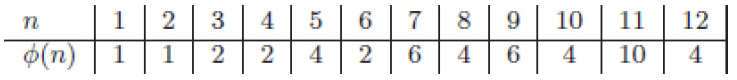
\includegraphics[width=0.7\linewidth]{figures/euler_phi_func.png}
    \caption{The first 12 values of $\phi(n)$.}
    \label{euler_phi_func}
\end{figure}

\noindent\fbox{\parbox{\linewidth}{
\begin{theorem}
Let $G$ be cyclic, $|G|=n$. If $d \mid n, d \in \mathbb{N}$, then the number of elements $a \in G: |a|=d$ is $\phi(d)$.
\end{theorem}
}}

\begin{proof}
    Let $G$ be cyclic, $|G|=n$. Assume that $d \mid n, d>0$, then by Theorem 4.3, there exists only one $H \leq G: |H| = d$. Let $H = \langle a \rangle$. Since by Corollary 4.2.3, $\langle a \rangle = \langle a^k \rangle \iff \gcd(d,k)=1$, and $|a^k| = |\langle a^k \rangle|  = \langle a \rangle = |a| = d$. It follows that $\phi(d)$ = the number of $k \in \mathbb{N}: k < d, \gcd(d,k)=1$ = the number of $a^k \in H: |a^k|=d$.
\end{proof}

\noindent\fbox{\parbox{\linewidth}{
\begin{corollary}
    Let $G$ be a group, $|G|=n$. Then the number of elements $a \in G: |a|=d$ is a multiple of $\phi(d)$.
\end{corollary}
}}

\begin{proof}
    Let $G$ be a group, $|G|=n$. If the number of elements $a \in G: |a|=d$ is 0, then since 0 is a multiple of $\phi(d)$, the statement is true. If $\exists a \in G: |a| = d$, then by Theorem 4.4, $\langle a \rangle$ has $\phi(d)$ elements of order $d$. 
    
    If all elements of order $d$ in $G$ are in $\langle a \rangle$, then the number of elements of order $d$ is a multiple of $\phi(d)$. If $\exists b \in G: |b|=d, b \notin \langle a \rangle$, then $\langle b \rangle$ has $\phi(d)$ elements of order $d$. So there are $2\phi(d)$ elements of order $d$ in $G$ provided $\langle a \rangle$ and $\langle b \rangle$ have no elements of order $d$ in common. If $\exists c \in \langle a \rangle, \langle b \rangle: |c|=d$, then $\langle a \rangle = \langle b \rangle = \langle c \rangle$, so $b \in \langle a \rangle$, a contradiction. Continuing in this fashion, the number of elements of order $d$ in $G$ is a multiple of $\phi(d)$.
\end{proof}

Theorem 4.4 together with the two number theorem properties that for any prime $p$,
\begin{enumerate}
    \item $\phi(p^n)=p^n-p^{n-1}$, and
    \item $\phi(p_1^{k_1}p_2^{k_2} \dots p_m^{k_m}) = \phi(p_1^{k_1})\phi(p_2^{k_2}) \dots \phi(p_m^{k_m})$, $p_1,p_2,\dots,p_m$ are distinct,
\end{enumerate}
simplify the task of determining orders of element in $U(n)$ and whether or not $U(n)$ is cyclic.

\begin{example}
    Let $U(n), n>2$ be cyclic. Since $2 \mid |U(n)| = \phi(n)$, by Theorem 4.3, there exists only one $H \leq U(n): |H| = 2$. Since $\langle -1 \rangle = \langle n-1 \rangle \leq U(n)$ and $|\langle n-1 \rangle| = |\langle -1 \rangle| = |-1| = 2$, it follows that $\langle n-1 \rangle$ is the only subgroup of order 2 of $U(n)$. But in $U(80), 9^2 = 1 \implies |9|=|\langle 9 \rangle| = 2, \langle 9 \rangle \neq \langle 79 \rangle$, and in $U(120), 11^2 = 1 \implies |11|=|\langle 11 \rangle| = 2, \langle 11 \rangle \neq \langle 119 \rangle$. Hence $U(80),U(120)$ are not cyclic. 
\end{example}

\section{Permutation Groups}
\subsection{Definition and Notation}
\fbox{\parbox{\linewidth}{
\begin{definition}
    A \textit{permutation} of a set $A$ is a one-to-one and onto function $f: A \to A$. A \textit{permutation group} of a set $A$ is a set of permutation of $A$ that forms a group under function composition.
\end{definition}
}}

\begin{note}
    For example, define a permutation $\alpha$ of the set $\{1,2,3,4\}$ as
\begin{equation*}
    \alpha(1) = 2, \alpha(2) = 3, \alpha(3) = 1, \alpha(4)=4.
\end{equation*}
or in array form
\begin{equation*}
    \alpha = 
    \begin{bmatrix}  
        1 & 2 & 3 & 4 \\
        2 & 3 & 1 & 4
    \end{bmatrix}.
\end{equation*}
Similarly, the permutation $\beta$ of $\{1,2,3,4,5,6\}$ can be defined as
\begin{equation*}
    \beta =
    \begin{bmatrix}
        1 & 2 & 3 & 4 & 5 & 6 \\
        5 & 3 & 1 & 6 & 2 & 4
    \end{bmatrix}.
\end{equation*}
Let 
\begin{equation*}
    \sigma =
    \begin{bmatrix}
        1 & 2 & 3 & 4 & 5 \\
        2 & 4 & 3 & 5 & 1
    \end{bmatrix},
    \gamma =
    \begin{bmatrix}
        1 & 2 & 3 & 4 & 5 \\
        5 & 4 & 1 & 2 & 3
    \end{bmatrix},
\end{equation*}
Figure \ref{composition_permutation} shows the composition of permutations $\sigma$ and $\gamma$. Since $(\gamma\sigma)(1)=\gamma(\sigma(1)) = \gamma(2) = 4$, so $\gamma\sigma$ maps 1 to 4.
\end{note}
\begin{figure}[!htbp]
    \centering
    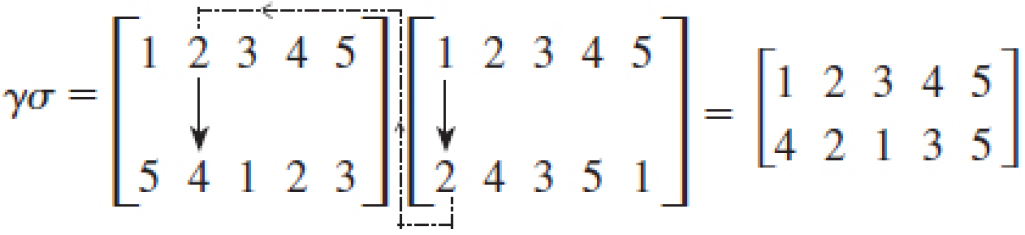
\includegraphics[width=0.7\linewidth]{figures/composition_permutation.png}
    \caption{Composition of permutations $\sigma$ and $\gamma$.}
    \label{composition_permutation}
\end{figure}

\begin{example}
    Let $S_3$ be the set of all permutations of $\{1,2,3\}$. Then $S_3$ under function composition is a group with six elements. The six elements are
    \begin{equation*}
        \epsilon = 
        \begin{bmatrix}
            1 & 2 & 3 \\
            1 & 2 & 3
        \end{bmatrix},
        \alpha = 
        \begin{bmatrix}
            1 & 2 & 3 \\
            2 & 3 & 1
        \end{bmatrix},
        \alpha^2 = 
        \begin{bmatrix}
            1 & 2 & 3 \\
            3 & 1 & 2
        \end{bmatrix},
    \end{equation*}
    \begin{equation*}
        \beta = 
        \begin{bmatrix}
            1 & 2 & 3 \\
            1 & 3 & 2
        \end{bmatrix},
        \alpha\beta = 
        \begin{bmatrix}
            1 & 2 & 3 \\
            2 & 1 & 3
        \end{bmatrix},
        \alpha^2\beta = 
        \begin{bmatrix}
            1 & 2 & 3 \\
            3 & 2 & 1
        \end{bmatrix}.
    \end{equation*}
    Since
    \begin{equation*}
        \beta\alpha =
        \begin{bmatrix}
            1 & 2 & 3 \\
            3 & 2 & 1
        \end{bmatrix}
        = \alpha^2\beta \neq \alpha\beta,
    \end{equation*}
    $S_3$ is non-Abelian. The relation $\beta\alpha = \alpha^2\beta$ can be used to compute other products in $S_3$ without resorting to the arrays. For example
    \begin{equation*}
        \beta\alpha^2 = (\beta\alpha)\alpha = (\alpha^2\beta)\alpha = \alpha^2(\beta\alpha) = \alpha^2(\alpha^2\beta) = \alpha^4\beta = \alpha\beta.
    \end{equation*}
\end{example}
 
 \begin{example}
     $S_n$ is the set of all permutations of a set of $n$ elements $A=\{1,2,\dots,n\}$ called \textit{the symmetric group of degree $n$}. Elements of $S_n$ have the form
     \begin{equation*}
         \alpha = 
         \begin{bmatrix}
             1 & 2 & \dots & n \\
             \alpha(1) & \alpha(2) & \dots & \alpha(n)
         \end{bmatrix}.
     \end{equation*}
     Since $\alpha$ is one-to-one, there are $n$ choices for $\alpha(1)$, $n-1$ choices for $\alpha(2)$, \dots, 1 choice for $\alpha(n)$. So $S_n$ has $n!=n\cdot(n-1)\cdot \dots \cdot 2\cdot1$ elements and $|S_n|=n!$. $S_n$ is non-Abelian when $n \geq 3$, since any permutation $\alpha$ only commute with the identity permutation $\epsilon$, i.e. $\epsilon\alpha = \alpha\epsilon$.
 \end{example}
 
 \begin{example}
    Associate each motion in $D_4$ with the permutation of the location of each of the four corners of a square.  
 \end{example}
 
 \subsection{Cycle Notation}
 \begin{note}
    Consider the permutation
 \begin{equation*}
     \alpha =
     \begin{bmatrix}
         1 & 2 & 3 & 4 & 5 & 6 \\
         2 & 1 & 4 & 6 & 5 & 3
     \end{bmatrix}.
 \end{equation*}
 Figure \ref{cycle_notation} shows the cycle notation of $\alpha$. Figure \ref{cycle_notation} can also be expressed as $\alpha = (1,2)(3,4,6)(5)$ or $\alpha = (12)(346)(5)$.
 \begin{figure}[!htbp]
     \centering
     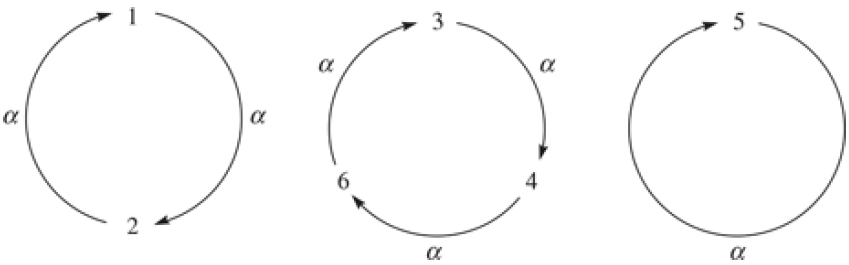
\includegraphics[width=0.7\linewidth]{figures/cycle_notation.png}
     \caption{Cycle notation of $\alpha$.}
     \label{cycle_notation}
 \end{figure}
 
 As a second example, consider
 \begin{equation*}
     \beta =
     \begin{bmatrix}
         1 & 2 & 3 & 4 & 5 & 6 \\
         5 & 3 & 1 & 6 & 2 & 4
     \end{bmatrix}.
 \end{equation*}
 In cycle notation, $\beta = (2,3,1,5)(6,4)$ or $(4,6)(3,1,5,2)$. An expression of the form $(a_1,a_2,\dots,a_m)$ is called a \textit{cycle of length $m$} or an \textit{$m$-cycle}.
 
 A multiplication of cycle can be performed by thinking of a cycle as a permutation that fixes any symbol not appearing in the cycle. So the cycle $(4,6)$ can be thought of as the permutation $\begin{bmatrix}
     1 & 2 & 3 & 4 & 5 & 6 \\
     1 & 2 & 3 & 6 & 5 & 4
 \end{bmatrix}$.
 Then the multiplication of cycles can be thought of as composition of permutations in array form. Let $\alpha=(13)(27)(456)(8), \beta=(1237)(648)(5) \in S_8$. Then $\alpha\beta=(13)(27)(456)(8)(1237)(648)(5)$. One proceeds by treating each of the cycles of $\alpha\beta$ as a function $f:\{1,\dots,8\} \to \{1,\dots,8\}$ and use function composition. Each cycle that does not contain a symbol fixes that symbol. For example, for $\alpha\beta(1)$, (5) fixes 1, then (648) fixes 1, then (1237) maps 1 to 2, then (8) fixes 2, then (456) fixes 2, then (27) maps 2 to 7, and lastly (13) fixes 7. So $\alpha\beta(1)=7$. Thus one begins with $\alpha\beta=(17\dots)\cdots$. Figure \ref{alpha_beta(1)} shows $\alpha\beta(1)$.
 
 \begin{figure}[!htbp]
     \centering
     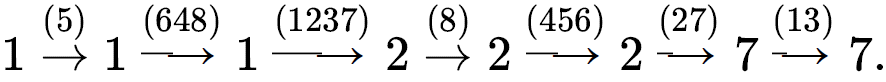
\includegraphics[width=0.5\linewidth]{figures/alphabeta(1).png}
     \caption{$\alpha\beta(1)=7$.}
     \label{alpha_beta(1)}
 \end{figure}
 
 Then, for $\alpha\beta(7)$, (5) fixes 7, (648) fixes 7, (1237) maps 7 to 1, (8) fixes 1, (456) fixes 1, (27) fixes 1, and (13) maps 1 to 3, so $\alpha\beta(7)=3$. Figure \ref{alpha_beta(7)} shows $\alpha\beta(7)=3$. Hence, $\alpha\beta = (173\dots)\cdots$. Eventually, $\alpha\beta = (1732)(48)(56)$.
 
 \begin{figure}[!htbp]
     \centering
     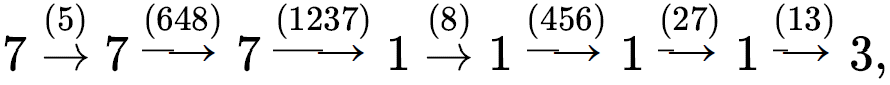
\includegraphics[width=0.5\linewidth]{figures/alphabeta(7).png}
     \caption{$\alpha\beta(7)=3$.}
     \label{alpha_beta(7)}
 \end{figure}
 
 For another example, if 
 \begin{equation*}
     \alpha = 
     \begin{bmatrix}
        1 & 2 & 3 & 4 & 5 \\
        2 & 1 & 3 & 5 & 4 
     \end{bmatrix},
     \beta = 
     \begin{bmatrix}
        1 & 2 & 3 & 4 & 5 \\
        5 & 4 & 1 & 2 & 3 
     \end{bmatrix}.
 \end{equation*}
 Then in cycle notation, $\alpha=(12)(3)(45), \beta=(153)(24), \alpha\beta=(12)(3)(45)(153)(24)$. For $\alpha\beta(1)$, (24) fixes 1, (153) maps 1 to 5, (45) maps 5 to 4, (3) fixes 4, and (12) fixes 4. So $\alpha\beta(1)=4$. Eventually, $\alpha\beta = (14)(253)$.
 
 One can convert $\alpha\beta$ back to array form without converting each cycle of $\alpha\beta$ back to array form by observing that (14) means $1 \to 4, 4 \to 1$; (253) means $2 \to 5, 5 \to 3, 3 \to 2$.
 
 Any missing element in a cycle is mapped to itself. So $\alpha = (12)(3)(45)=(12)(45)$ and the identity permutation
 \begin{equation*}
     \epsilon = 
     \begin{bmatrix}
        1 & 2 & 3 & 4 & 5 \\
        1 & 2 & 3 & 4 & 5 
     \end{bmatrix}
 \end{equation*}
 in cycle form is $\epsilon = (1) = (2) = (3) = (4) = (5)$.
  \end{note}
 
 \subsection{Properties of Permutations}
 \fbox{\parbox{\linewidth}{
 \begin{theorem}
    Every permutation of a finite set can be expressed as a cycle or as a product of disjoint cycles. \end{theorem}
 }}
 
 \begin{proof}
     Let $\alpha$ be a permutation on $A = \{1,2,\dots,n\}$. To write $\alpha$ in disjoint form, choose any member of $A$, say $a_1$, and let
     \begin{equation*}
         a_2 = \alpha(a_1), a_3 = \alpha(a_2) = \alpha(\alpha(a_1)) = \alpha^2(a_1), a_4 = \alpha^3(a_1), \dots.
     \end{equation*}
     Since $A$ is finite, eventually there will be a repetition 
     \begin{equation*}
         a_{m+1} = \alpha^m(a_1) = a_1, m \in \mathbb{N}.
     \end{equation*}
     If 
     \begin{equation*}
         \alpha^i(a_1) = \alpha^j(a_1), i,j \in \mathbb{N},i<j,
     \end{equation*}
     then $a_1 = \alpha^m(a_1) = \alpha^{j-i}(a_1)$. The relationship among $a_1,a_2,\dots,a_m$ is expressed as
     \begin{equation*}
         \alpha = (a_1,a_2,\dots,a_m)\cdots.
     \end{equation*}
     The three dots at the end indicate that $A$ may have not been exhausted in this process. If so, then choose any element $b_1 \in A$ not in the first cycle and repeat the process until 
     \begin{equation*}
         b_{k+1} = b_1 = \alpha^k(b_1), k \in \mathbb{N}.
     \end{equation*}
     If 
     \begin{equation*}
         \alpha^i(a_1)=\alpha^j(b_1), i,j \in \mathbb{N},
     \end{equation*}
     then 
     \begin{equation*}
         \alpha^{i-j}(a_1)=\alpha^j\alpha^{-j}(b_1) = \epsilon(b_1) = b_1 \implies b_1 = a_t, t \in \mathbb{N}.
     \end{equation*}
     This contradicts that $b_1$ is not in the first cycle. Hence the new cycle has no elements in common with the first cycle. Continuing the process until $A$ is exhausted, the permutation is expressed as
     \begin{equation*}
         \alpha = (a_1,a_2,\dots,a_m)(b_1,b_2,\dots,b_k)\cdots(c_1,c_2,\dots,c_s).
     \end{equation*}
 \end{proof}
 
 \noindent\fbox{\parbox{\linewidth}{
 \begin{theorem}
    If the pair of cycles $\alpha=(a_1,a_2,\dots,a_m),\beta = (b_1,b_2,\dots,b_n)$ have no entries in common, then $\alpha\beta = \beta\alpha$.
 \end{theorem}
 }}
 
 \begin{proof}
     Let $\alpha, \beta$ be the permutation of the set
     \begin{equation*}
         S = \{a_1,a_2,\dots,a_m,b_1,b_2,\dots,b_n,c_1,c_2,\dots,c_k\},
     \end{equation*}
     where $c$'s are the members of $S$ left fixed by both $\alpha, \beta$ (there may not be any $c$'s). Let $a_i$ be an arbitrary $a$ element, then
     \begin{equation*}
         (\alpha\beta)(a_i) = \alpha(\beta(a_i)) = \alpha(a_i) = a_{i+1},
     \end{equation*}
     since $\beta$ fixes all $a$ elements. $a_{i+1} = a_1$ if $i=m$. Similarly,
     \begin{equation*}
         (\beta\alpha)(a_i) = \beta(\alpha(a_i)) = \beta(a_{i+1}) = a_{i+1}.
     \end{equation*}
     Hence $\alpha\beta = \beta\alpha$ for all $a$ elements. The same can be applied to all $b$ elements. Let $c_i$ be an arbitrary $c$ element, then
     \begin{equation*}
         (\alpha\beta)(c_i) = \alpha(\beta(c_i)) = \alpha(c_i) = c_i,
     \end{equation*}
     and
     \begin{equation*}
         (\beta\alpha)(c_i) = \beta(\alpha(c_i)) = \beta(c_i) = c_i.
     \end{equation*}
     So $\alpha\beta = \beta\alpha$ for all $c$ elements. Hence $\alpha\beta = \beta\alpha$ for all elements in $S$.
 \end{proof}
 
 \noindent\fbox{\parbox{\linewidth}{
 \begin{theorem}
    Let $\alpha$ be a permutation of a finite set written in disjoint cycle form. Then $|\alpha|=\lcm(\text{the lengths of the cycles})$.
 \end{theorem}
 }}
 
 \begin{proof}
     Let $\alpha = (a_1,a_2,\dots,a_n)$ be an arbitrary cycle of length $n$. Then
     \begin{align*}
         \alpha(a_1) &= a_2, \\
         \alpha(a_2) &= \alpha(\alpha(a_1)) = \alpha^2(a_1) = a_3. \\
         \alpha(a_3) &= \alpha(\alpha^2(a_1)) = \alpha^3(a_1) = a_4, \\
         & \vdots \\
         \alpha(a_n) &= \alpha^n(a_1) = a_{n+1} = a_1.
     \end{align*}
     So $\alpha^n(a_i) = a_i, i \in \{1,\dots,n\} \implies \alpha^n = \epsilon$ and $|\alpha| = |(a_1,a_2,\dots,a_n)| = n$. Hence a cycle of $n$ length has order $n$.
     
     Let $\gamma = \alpha\beta = (a_1,\dots,a_m)(b_1,\dots,b_n)$ be a permutation of a finite set in disjoint cycle form, and let $k=\lcm(m,n)$. WTS $|\gamma| = |\alpha\beta| = \lcm(m,n)=k$. 
     
     Since $|\alpha|=m,|\beta|=n$ and $m,n \mid k$, by Theorem 4.1,
     \begin{align*}
         \alpha^k = \alpha^0 = \epsilon &\iff m \mid (k-0) = k, \\
         \beta^k = \beta^0 = \epsilon &\iff n \mid (k-0) = k.
     \end{align*}
     Hence $\alpha^k = \epsilon, \beta^k = \epsilon$. Since $\alpha,\beta$ are disjoint, by Theorem 5.2, $\alpha\beta=\beta\alpha$. So
     \begin{equation*}
         \gamma^k = (\alpha\beta)^k = \alpha^k\beta^k = \epsilon\epsilon = \epsilon
     \end{equation*}
     and $|\gamma|=t \leq k$. 
     
     By Theorem 4.1, 
     \begin{equation*}
         \gamma^k = \epsilon \iff |\gamma| = t \mid k,
     \end{equation*}
     and
     \begin{equation*}
         |\gamma| = |\alpha\beta| = t \implies \gamma^t = (\alpha\beta)^t = \alpha^t\beta^t = \epsilon.
     \end{equation*}
     Since $\alpha,\beta$ are disjoint, it follows that 
     \begin{align*}
         \alpha^k(b_i) &= b_i, i \in \{1,\dots,n\}, \\
         \beta^k(a_i) &= a_i, i \in \{1,\dots,m\}.
     \end{align*}
     Since $\gamma^t = \alpha^t\beta^t = \epsilon$, it follows that
     \begin{align*}
         \gamma^t(a_i) &= (\alpha^t\beta^t)(a_i) = \epsilon(a_i) = a_i, i \in \{1,\dots,m\}, \\
         \gamma^t(b_i) &= (\alpha^t\beta^t)(b_i) = \epsilon(b_i) = b_i, i \in \{1,\dots,n\}. 
     \end{align*}
     This is true iff $\alpha^t=\epsilon, \beta^t=\epsilon$. By Theorem 4.1, 
     \begin{align*}
         \alpha^t = \alpha^0 = \epsilon &\iff m \mid (t-0) = t, \\
         \beta^t = \beta^0 = \epsilon &\iff n \mid (t-0) = t,
     \end{align*}
     so $t$ is a common multiple of $m,n$. Since $k = \lcm(m,n)$, it follows that $t \geq k$. So
     \begin{equation*}
         t \geq k, t \leq k \implies t = k
     \end{equation*}
     and hence $|\gamma| = t = k$.
     
     The general cases involving more than two cycles can be proved in a similar manner.
 \end{proof}
 
 \begin{example}
 \begin{align*}
     |(132)(45)| &= \lcm(3,2) = 6, \\
     |(1432)(56)| &= \lcm(4,2) = 4, \\
     |(123)(456)(78)| &= \lcm(3,3,2) = 6, \\
     |(123)(145)| &= |(14523)| = 5. 
 \end{align*}
 \end{example}
 
 \begin{example}
    Determine the orders of the $7! = 5040$ elements of $S_7$. For convenience, denote an $n$-cycle by $(\underline{n})$. Then, arranging all possible disjoint cycle structures of elements of $S_7$ according to longest cycle lengths left to right,
    \begin{align*}
        (\underline{7}), \\
        (\underline{6})(\underline{1}), \\
        (\underline{5})(\underline{2}), \\
        (\underline{5})(\underline{1})(\underline{1}), \\
        (\underline{4})(\underline{3}), \\
        (\underline{4})(\underline{2})(\underline{1}), \\
        (\underline{4})(\underline{1})(\underline{1})(\underline{1}), \\
        (\underline{3})(\underline{3})(\underline{1}), \\
        (\underline{3})(\underline{2})(\underline{2}), \\
        (\underline{3})(\underline{2})(\underline{1})(\underline{1}), \\
        (\underline{3})(\underline{1})(\underline{1})(\underline{1})(\underline{1}), \\
        (\underline{2})(\underline{2})(\underline{2})(\underline{1}) \\
        (\underline{2})(\underline{2})(\underline{1})(\underline{1})(\underline{1}), \\
        (\underline{2})(\underline{1})(\underline{1})(\underline{1})(\underline{1})(\underline{1}), \\
        (\underline{1})(\underline{1})(\underline{1})(\underline{1})(\underline{1})(\underline{1})(\underline{1}).
    \end{align*}
    By Theorem 5.3, the orders of the elements of $S_7$ are
    \begin{align*}
        7, \\
        \lcm(6,1) &= \lcm(3,2,2) = \lcm(3,2,1,1) = 6, \\
        \lcm(5,2) &= 10, \\
        \lcm(5,1,1) &= 5, \\
        \lcm(4,3) &= 12, \\
        \lcm(4,2,1) &= \lcm(4,1,1,1) = 4, \\
        \lcm(3,3,1) &= \lcm(3,1,1,1,1) = 3, \\
        \lcm(2,2,2,1) &= \lcm (2,2,1,1,1) = \lcm(2,1,1,1,1,1) = 2, \\
        \lcm(1,1,1,1,1,1,1) &= 1.
    \end{align*}
 \end{example}
 
 \begin{example}
    Determine the number of elements of order 12 in $S_7$. Since $\lcm(4,3)=12$, by Theorem 5.2 and 5.3, only the number of permutations with disjoint cycle form $(a_1a_2a_3a_4)(a_5a_6a_7)$ is needed to be counted. First consider the cycle $(a_1a_2a_3a_4)$. There are $7\cdot6\cdot5\cdot4$ ways of choosing 4 out of 7 entries, but each choice of the cycle $(a_1a_2a_3a_4)$ is counted four times. For example, 
    \begin{equation*}
        (2741) = (1274) = (4127) = (7412).
    \end{equation*}
    Similarly, there are $3\cdot2\cdot1$ ways of choosing 3 out of 7 entries for $(a_5a_6a_7)$, but each choice of $(a_5a_6a_7)$ is counted three times. Hence, there are
    \begin{equation*}
        \frac{(7\cdot6\cdot5\cdot4)(3\cdot2\cdot1)}{(4)(3)} = 420
    \end{equation*}
    elements of order 12 in $S_7$.
 \end{example}
 
 \begin{example}
    Determine the number of elements of order 3 in $S_7$. Since $\lcm(3,3,1) = \lcm(3,1,1,1,1) = 3$, by Theorem 5.2 and 5.3, the elements of order 3 in $S_7$ have the disjoint cycle form
    \begin{equation*}
        (a_1a_2a_3)(a_4a_5a_6)(a_7) \quad \text{and} \quad (a_1a_2a_3)(a_4)(a_5)(a_6)(a_7).
    \end{equation*}
    or
    \begin{equation*}
        (a_1a_2a_3)(a_4a_5a_6) \quad \text{and} \quad (a_1a_2a_3).
    \end{equation*}
    For $(a_1a_2a_3)(a_4a_5a_6)$, there are $(7\cdot6\cdot5)/3$ ways of creating $(a_1a_2a_3)$ and there are $(4\cdot3\cdot2)/3$ ways of creating $(a_4a_5a_6)$. But $(7\cdot6\cdot5)/3$ and $(4\cdot3\cdot2)/3$ count $(a_1a_2a_3)(a_4a_5a_6)$ and $(a_4a_5a_6)(a_1a_2a_3)$ as distinct elements when they are identical. So there are
    \begin{equation*}
        \frac{(7\cdot6\cdot5)(4\cdot3\cdot2)}{(3)(3)(2)} = 280
    \end{equation*} elements of order 3 in $S_7$ with disjoint cycle form $(a_1a_2a_3)(a_4a_5a_6)$.
    
    For $(a_1a_2a_3)$, there are $(7\cdot6\cdot5)/3$ ways of creating $(a_1a_2a_3)$. So there are $(7\cdot6\cdot5)/3=70$ elements of order 3 in $S_7$ with the distinct cycle form $(a_1a_2a_3)$. Hence there are $280+70=350$ elements of order 3 in $S_7$.
 \end{example}
 
 \noindent\fbox{\parbox{\linewidth}{
 \begin{theorem}
    Every permutation in $S_n, n>1$ is a product of 2-cycle.
 \end{theorem}
 }}
 
 \begin{proof}
     The identity permutation $\epsilon$ can be expressed as $(12)(12)$. So $\epsilon$ can be expressed as a product of 2-cycle. By Theorem 5.1, every permutation can be written in the disjoint cycle form
     \begin{equation*}
         (a_1 \dots a_k)(b_1 \dots b_t)(c_1 \dots c_s).
     \end{equation*}
     This is the same as
     \begin{align*}
         (a_1a_k)(a_1a_{k-1})(a_1a_{k-2}) \dots (a_1a_2)(b_1b_t)(b_1b_{t-1})(b_1b_{t-2}) \dots (b_1b_2) \\
         \dots (c_1c_s)(c_1c_{s-1})(c_1c_{s-2}) \dots (c_1c_2).
     \end{align*}
 \end{proof}
 
 \begin{example}
 \begin{align*}
     (12345) &= (15)(14)(13)(12) \\
    (1632)(457) &= (12)(13)(16)(47)(45)
 \end{align*}
 \end{example}
 
 \begin{example}
 \begin{align*}
     (12345) &= (54)(53)(52)(51) \\
     (12345) &= (54)(52)(21)(25)(23)(13)
 \end{align*}
 \end{example}
 
 \noindent\fbox{\parbox{\linewidth}{
 \begin{lemma}
     If $\epsilon=\beta_1\beta_2\dots\beta_r$, where $\beta_1,\beta_2,\dots,\beta_r$ are 2-cycles, then $r$ is even.
 \end{lemma}
 }}
 
 \begin{proof}
     
 \end{proof}
 
 \noindent\fbox{\parbox{\linewidth}{
 \begin{theorem}
    Let $\alpha$ be a permutation. If
    \begin{equation*}
        \alpha = \beta_1\beta_2\dots\beta_r \quad \text{and} \quad \alpha = \gamma_1\gamma_2\dots\gamma_s,
    \end{equation*}
    where $\beta,\gamma$ are all 2-cycles, then $r,s$ are both even or both odd. 
 \end{theorem}
 }}
 
 \begin{proof}
     Let $\alpha$ be a permutation and let
    \begin{equation*}
        \alpha = \beta_1\beta_2\dots\beta_r \quad \text{and} \quad \alpha = \gamma_1\gamma_2\dots\gamma_s,
    \end{equation*}
    where $\beta,\gamma$ are all 2-cycles. Then since the inverse of an 2-cycle is itself,
    \begin{align*}
        \alpha = \beta_1\beta_2\dots\beta_r = \gamma_1\gamma_2\dots\gamma_s \implies \epsilon &= \gamma_1\dots\gamma_s\beta_1^{-1}\dots\beta_r^{-1} \\
        &= \gamma_1\dots\gamma_s\beta_1\dots\beta_r.
    \end{align*}
    By Lemma 5.4.1, if $\epsilon = \beta_1\dots\beta_t$, where all $\beta$ are  2-cycles, then $t$ is even. So $t=r+s$ is even $\iff$ $r,s$ are both even or both odd. 
 \end{proof}
 
 \noindent\fbox{\parbox{\linewidth}{
 \begin{definition}
     Let $\alpha$ be a permutation and let $\alpha = \beta_1\dots\beta_r$ where all $\beta_i$'s are 2-cycles. If $r$ is even then $\alpha$ is an \textit{even} permutation. If $r$ is odd then $\alpha$ is an \textit{odd} permutation. 
 \end{definition}
 }}
 \\ \\
 \fbox{\parbox{\linewidth}{
 \begin{theorem}
    The set of even permutations in $S_n$ is a subgroup of $S_n$.
 \end{theorem}
 }}
 
 \begin{proof}
     Let $A \in S_n$ be the set of even permutations. Let $\alpha,\beta \in A$ be arbitrary. So
     \begin{equation*}
         \alpha = \gamma_1\dots\gamma_r, \beta = \sigma_1\dots\sigma_s,
     \end{equation*}
     where $\gamma$'s and $\sigma$'s are 2-cycles and $r,s$ are even. Since
     \begin{equation*}
         \alpha\beta = \gamma_1\dots\gamma_r\sigma_1\dots\sigma_s
     \end{equation*}
     and $r+s$ is even, it follows that $\alpha\beta \in A$. Next,
     \begin{align*}
         \alpha\alpha^{-1} &= \epsilon, \\
         \gamma_1\dots\gamma_r\alpha^{-1} &= \epsilon, \\
         \alpha^{-1} &= \gamma_1^{-1}\dots\gamma_r^{-1}\epsilon \\
         &= \gamma_1^{-1}\dots\gamma_r^{-1} \\
         &= \gamma_1\dots\gamma_r \\
         &= \alpha \in A.
     \end{align*}
     Since $\alpha,\beta \in A \implies \alpha\beta \in A$ and $\alpha \in A \implies \alpha^{-1} \in A$, by Theorem 3.2, $A \leq S_n$.
 \end{proof}
 
 \noindent\fbox{\parbox{\linewidth}{
 \begin{definition}
     The group of even permutation of $n$ symbols is denoted by $A_n$ and is called the \textit{alternating group of degree $n$}.
 \end{definition}
 }}
 \\ \\ \\
 \fbox{\parbox{\linewidth}{
 \begin{theorem}
    Let $A_n$ be an alternating group of degree $n$. Then
     \begin{equation*}
         |A_n| = n!/2, n>1.
     \end{equation*}
 \end{theorem}
 }}
 
 \begin{proof}
     For each odd permutation $\alpha$, the permutation $(12)\alpha$ is even. By the cancellation property, $(12)\alpha \neq (12)\beta$ when $\alpha \neq \beta$. So there are at least as many even permutations as there are odd ones. For each even permutation $\alpha$, the permutation $(12)\alpha$ is odd. By the cancellation property, $(12)\alpha \neq (12)\beta$ when $\alpha \neq \beta$. So there are at least as many odd permutations as there are even ones. Hence the numbers of even and odd permutations are the same. Since $|S_n| = n!$, it follows that $|A_n| = n!/2$.
 \end{proof}
 
 \begin{figure}[!ht]
     \centering
     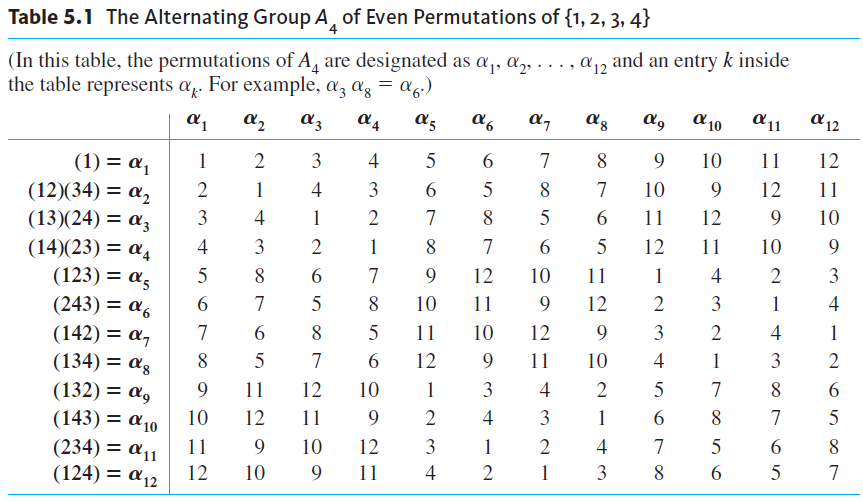
\includegraphics[width=\linewidth]{figures/A_4_table.png}
     \caption{}
     \label{A_4_table}
 \end{figure}
 
 \section{Isomorphism}
 \subsection{Definition and Examples}
 \fbox{\parbox{\linewidth}{
 \begin{definition}
 \label{isomorphism definition}
     Let $G,\overline{G}$ be two groups. Let $\phi:G \to \overline{G}$ be a function s.t.
     \begin{enumerate}
         \item $\forall a,b \in G, \phi(a) = \phi(b) \implies a = b$ (one-to-one),
         \item $\forall \overline{a} \in \overline{G}, \exists a \in G: \phi(a) = \overline{a}$ (onto),
         \item $\forall a,b \in G, \phi(ab) = \phi(a)\phi(b)$ (preservation of operations),
     \end{enumerate}
     then $\phi$ is an isomorphism from $G$ to $\overline{G}$.
     \\ \\
     If there is an isomorphism from $G$ to $\overline{G}$, then $G$ and $\overline{G}$ are isomorphic, denoted $G \approx \overline{G}$.
 \end{definition}
 }}
 \\ \\
 Figure \ref{isomorphism} shows the visualization of Definition \ref{isomorphism definition}. Figure \ref{isomophism_operation_tables} shows the operation tables for $G$ and $\overline{G}$. The operation table for $\overline{G}$ can be obtained by replacing each entry $x$ in the operation table for $G$ by $\phi(x)$. Figure \ref{isomorphism_operations} shows the four cases of operations of $G$ and $\overline{G}$ involving $\cdot$ and +.
 
 \begin{figure}[!htbp]
     \centering
     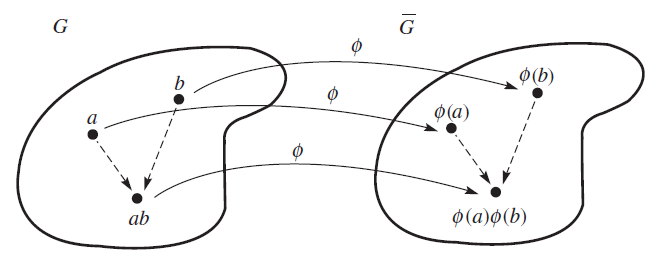
\includegraphics[width=0.8\linewidth]{figures/isomorphism.png}
     \caption{}
     \label{isomorphism}
 \end{figure}
 
 \begin{figure}[!htbp]
     \centering
     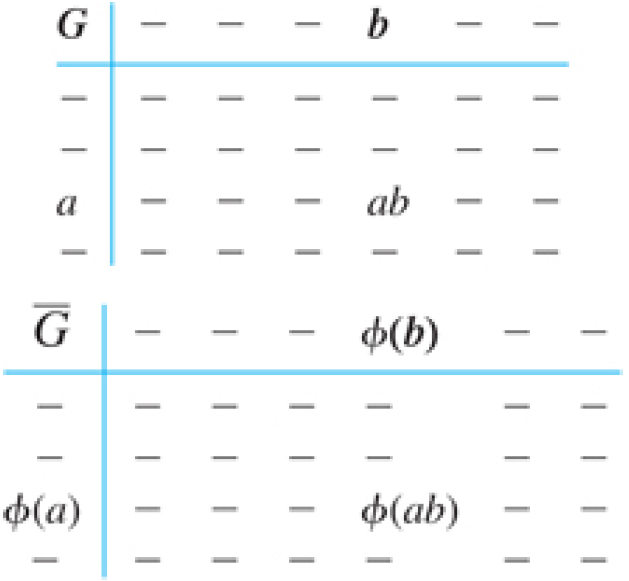
\includegraphics[width=0.4\linewidth]{figures/isomophism_table.png}
     \caption{Operation tables for $G$ and $\overline{G}$. The operation table for $\overline{G}$ can be obtained by replacing each entry $x$ in the operation table for $G$ by $\phi(x)$.}
     \label{isomophism_operation_tables}
 \end{figure}
 
 \begin{figure}[!htbp]
     \centering
     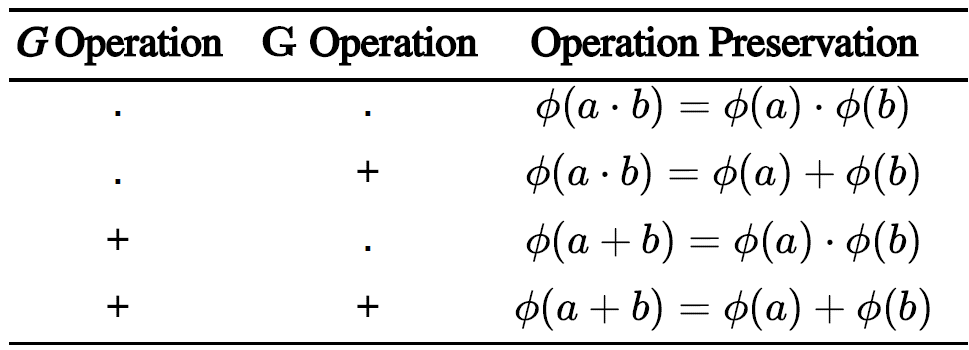
\includegraphics[width=0.7\linewidth]{figures/isomophism_operations.png}
     \caption{The four cases of operations of $G$ and $\overline{G}$ involving $\cdot$ and +}.
     \label{isomorphism_operations}
 \end{figure}
 
 There are four steps involved in proving that $G \approx \overline{G}$.
 \begin{enumerate}
     \item \textbf{Mapping.} Define a function $\phi: G \to \overline{G}$.
     \item \textbf{1-1.} Show that $\forall a,b \in G, \phi(a) = \phi(b) \implies a=b$.
     \item \textbf{Onto.} Show that $\forall \overline{g} \in \overline{G}, \exists g \in G: \phi(g)=\overline{g}$.
     \item \textbf{Operation-Preserving.} Show that $\forall a,b \in G, 
     \phi(ab) = \phi(a)\phi(b)$.
 \end{enumerate}
 
 \begin{example}
    Let $G = (\mathbb{R},+)$ and $\overline{G} = (\mathbb{R}^+,\cdot)$. Show that $G \approx \overline{G}$ under $\phi(x)=2^x$.
    First, assume that $\forall a,b \in G, \phi(a) = \phi(b)$, then
    \begin{align*}
        \phi(a) &= \phi(b), \\
        2^a &= 2^b, \\
        \log_22^a &= \log_22^b, \\
        a &= b.
    \end{align*}
    So $\forall a,b \in G, \phi(a) = \phi(b) \implies a=b$. Next, let $b \in \overline{G}$ be arbitrary. WTS $\exists a \in G: 2^a = b$. Since
    \begin{align*}
        2^a &= b, \\
        \log_22^a &= \log_2b, \\
        a &= \log_2b,
    \end{align*}
    it follows that $\forall b \in \overline{G}, \exists a = \log_2b \in G: \phi(a) = 2^a = 2^{\log_2b} = b$. Finally, 
    \begin{equation*}
        \forall a,b \in G, \phi(a+b) = 2^{a+b} = 2^a \cdot 2^b = \phi(a) \cdot \phi(b).
    \end{equation*}
    Hence $G \approx \overline{G}$.
 \end{example}
 
 \begin{example}
    For any infinite cyclic group $G=\langle a \rangle, a \in G, |G| = \infty$, show that $G \approx (\mathbb{Z},+)$ under $\phi(a^k) = k, k \in \mathbb{Z}$. 
    
    First, assume that $\forall a^i, a^j \in G, \phi(a^i) = \phi(a^j)$, then
    \begin{align*}
        \phi(a^i) = \phi(a^j) \implies i = j.
    \end{align*}
    By Theorem 4.1 (i),
    \begin{equation*}
        |G| = |\langle a \rangle| = |a| = \infty \implies (a^i = a^j \iff i = j).
    \end{equation*}
    Hence $\forall a^i, a^j \in G, \phi(a^i) = \phi(a^j) \implies a^i = a^j$. Next, let $k \in \mathbb{Z}$ be arbitrary. Since $\langle a \rangle = \{a^k: k \in \mathbb{Z}\}$, it follows that $\exists a^k \in \langle a \rangle: \phi(a^k) = k$. Hence $\forall k \in \mathbb{Z}, \exists a^k \in \langle a \rangle: \phi(a^k) = k$. Finally, 
    \begin{align*}
        \phi(a^ia^j) = \phi(a^{i+j}) = i+j = \phi(a^i)+\phi(a^j).
    \end{align*}
    Hence, $G \approx (\mathbb{Z},+)$ under $\phi(a^k) = k, k \in \mathbb{Z}$.
    
    For any finite cyclic group $G = \langle a \rangle, a \in G, |G| = n$, show that $G \approx \mathbb{Z}_n$ under addition modulo $n$ under $\phi(a^k) = k \bmod n$.
    
    First, assume that $\forall a^i,a^j \in G, \phi(a^i) = \phi(a^j)$. Then
    \begin{align*}
        \phi(a^i) &= \phi(a^j), \\
        i \bmod n &= j \bmod n, \\
        (i-j) \bmod n &= 0 \implies n \mid (i-j).
    \end{align*}
    By Theorem 4.1 (ii),
    \begin{equation*}
        |a| = n \implies (a^i=a^j \iff n \bmod (i-j)).
    \end{equation*}
    Hence $\forall a^i,a^j \in G, \phi(a^i) = \phi(a^j) \implies a^i=a^j$. Next, since $|a| = n$, it follows that
    \begin{align*}
        a^0 &= a^n = a^{kn} = e, & a^{-1} &= a^{n-1} = a^{kn-1}, \\
        a^1 &= a^{n+1} = a^{kn+1}, & a^{-2} &= a^{n-2} = a^{kn-2}, \\
        a^2 &= a^{n+2} = a^{kn+2}, & a^{-3} &= a^{n-3} = a^{kn-3}, \\
        & \vdots & \vdots
    \end{align*}
    Hence $\forall a^k \in G, k \bmod n \in \{0,1,\dots,n-1\}$ and so $\forall x \in \mathbb{Z}_n, \exists a^k \in G: \phi(a^k)=k \bmod n=x$. Finally,
    \begin{align*}
        \phi(a^ia^j) = \phi(a^{i+j}) &= (i+j) \bmod n \\
        &= (i \bmod n + j \bmod n) \bmod n \\
        &= (\phi(a^i)+\phi(a^j)) \bmod n.
    \end{align*}
    Hence $G \approx \mathbb{Z}_n$ under addition modulo $n$ under $\phi(a^k) = k \bmod n$.
 \end{example}
 
 \begin{example}
    Let $G = (\mathbb{R},+)$. Show that $G$ and $G$ are not isomorphic under $\phi(x) = x^3$.
    
    First, assume $\forall a,b \in G, \phi(a) = \phi(b)$, then
    \begin{align*}
        \phi(a) = \phi(b) \implies a^3 = b^3 \implies a = b.
    \end{align*}
    Hence $\forall a,b \in G, \phi(a) = \phi(b) \implies a=b$. Next, since $\mathbb{I} \subseteq \mathbb{R}$ and
    \begin{equation*}
        y^3 = x \implies y = \sqrt[3]{x} \in \mathbb{I} \subseteq \mathbb{R},
    \end{equation*}
    it follows that $\forall x \in G, \exists y \in G: \phi(y) = y^3 = (\sqrt[3]{x})^3 = x$. But
    \begin{align*}
        \forall a,b \in G, \phi(a+b) = (a+b)^3 = a^3 + 3a^2b + 3ab^2 + b^3 \neq \phi(a) + \phi(b).
    \end{align*}
    Hence $\phi$ is not operation-preserving and $G$ and $G$ are not isomorphic under $\phi(x)=x^3$.
    
    \begin{example}
    \begin{enumerate}
        \item Show that $U(10)$ under multiplication modulo 10 $\approx \mathbb{Z}_4$ under addition modulo 4.
        
        Note that $\mathbb{Z_4}=\{1,2,3\},U(10)=\{1,3,7,9\}=\langle 3 \rangle$ and $|U(10)| = 4$. By Example 6.2, $U(10) \approx \mathbb{Z}_4$ under $\phi(3^k)=k \bmod 4$. First, assume that $\forall 3^i,3^j \in U(10), \phi(3^i) = \phi(3^j)$. Then
        \begin{align*}
            \phi(3^i) &= \phi(3^j), \\
            i \bmod 4 &= j \bmod 4, \\
            (i-j) \bmod 4 &= 0 \implies 4 \mid (i-j).
        \end{align*}
        By Theorem 4.1 (ii),
        \begin{equation*}
            |3| = 4 \implies (3^i=3^j \iff 4 \mid (i-j)).
        \end{equation*}
        Hence, 
        \begin{equation*}
            \forall 3^i,3^j \in U(10), \phi(3^i) = \phi(3^j) \implies 3^i=3^j.
        \end{equation*}
        Next, since
        \begin{align*}
            1 \in \mathbb{Z}_4, 1 &= \phi(3^1) = \phi(3^5) = \phi(3^{4k}), \\
            2 \in \mathbb{Z}_4, 2 &= \phi(3^{4k+2}), \\
            3 \in \mathbb{Z}_4, 3 &= \phi(3^{4k+3}),
        \end{align*}
        it follows that $\forall x \in \mathbb{Z}_4, \exists 3^k \in U(10): \phi(3^k) = x$. Finally,
        \begin{align*}
            \phi(3^i3^j) &= \phi(3^{i+j}) \\
            &= (i+j) \bmod 4 \\
            &= i \bmod 4 + j \bmod 4 \\
            &= \phi(3^i) + \phi(3^j).
        \end{align*}
        Hence, $U(10) \approx \mathbb{Z}_4$ under $\phi(3^k) = k \mod 4$.
        
        \item Similarly, $U(5) \approx \mathbb{Z}_4$.
    \end{enumerate}
    \end{example}
    
    \begin{example}
        There is no isomorphism from $\mathbb{Q}$ under addition to $\mathbb{Q}' = \mathbb{Q} \setminus \{0\}$ under multiplication. Since if $\mathbb{Q} \approx \mathbb{Q}'$, then there is an 1-1 and onto function s.t. $\exists a \in \mathbb{Q}: \phi(a)=-1$. But
        \begin{align*}
            -1 = \phi(a) = \phi\bigg(\frac{1}{2}a+\frac{1}{2}a\bigg) = \phi\bigg(\frac{a}{2}\bigg) \cdot \phi\bigg(\frac{a}{2}\bigg) = \bigg(\phi\bigg(\frac{a}{2}\bigg)\bigg)^2
        \end{align*}
        and there is no $x \in \mathbb{Q}': x^2 = -1$. Hence there is no isomorphism from $\mathbb{Q}$ under addition to $\mathbb{Q}'$ under multiplication.
    \end{example}
    
    \begin{example}
        Let $G = SL(2,\mathbb{R})$, the group of $2 \times 2$ matrices with determinant 1. Show that $G \approx G$ under $\phi_M(A) = MAM^{-1}, \forall A \in G$, $M$ is any $2 \times 2$ matrix with determinant 1. 
        
        First, let $A \in G$ be arbitrary, then
        \begin{equation*}
            \det(\phi_M(A)) = \det(MAM^{-1}) = (\det M)(\det A)(\det M^{-1}) = 1\cdot 1 \cdot 1 = 1.
        \end{equation*}
        Hence $\phi_M: G \to G$. Second, assume that $\forall A,B \in G, \phi_M(A) = \phi_M(B)$. Then
        \begin{align*}
            \phi_M(A) &= \phi_M(B), \\
            MAM^{-1} &= MBM^{-1}, \\
            M^{-1}MAM^{-1} &= M^{-1}MBM^{-1}, \\
            1 \cdot AM^{-1} &= 1 \cdot BM^{-1}, \\
            AM^{-1}M &= BM^{-1}M, \\
            A &= B.
        \end{align*}
        Hence, $\forall A,B \in G, \phi_M(A) = \phi_M(B) \implies A = B$. Next, let $B \in G$ be arbitrary. WTS $\exists A \in G: \phi(A) = MAM^{-1} = B$. Notice that
        \begin{equation*}
            \phi(A) = MAM^{-1} = B \implies A = M^{-1}BM.
        \end{equation*}
        Let $A = M^{-1}BM \in G$, then
        \begin{equation*}
            \phi(A) = MAM^{-1} = M(M^{-1}BM)M^{-1} = B.
        \end{equation*}
        Hence $\forall B \in G, \exists A \in G: \phi(A)=B$. Finally, 
        \begin{align*}
            \phi(AB) = MABM^{-1} = (MA)I(BM^{-1}) = (MAM^{-1})(MBM^{-1}) = \phi(A)\phi(B).
        \end{align*}
        Hence $G \approx G$ under $\phi(A) = MAM^{-1}, A \in G$.
    \end{example}
 \end{example}
 
 \subsection{Cayley's Theorem}
 \fbox{\parbox{\linewidth}{
 \begin{theorem}[Cayley's Theorem]
    Every group is isomorphic to a group of permutations.
 \end{theorem}
 }}
 
 \begin{proof}
     Let $G$ be an arbitrary group. Then for every $g \in G$, define a function $T_g:G \to G$ as
     \begin{equation*}
         \forall x \in G, T_g(x) = gx.
     \end{equation*}
     WTS $T_g$ is a permutation on the set of elements of $G$. Let $x_1,x_2 \in G$ be arbitrary, assume that $T_g(x_1) = T_g(x_2)$. Then,
     \begin{align*}
         T_g(x_1) &= T_g(x_2), \\
         gx_1 &= gx_2, \\
         g^{-1}gx_1 &= g^{-1}gx_2, \\
         x_1 &= x_2.
     \end{align*}
     Hence $\forall x_1, x_2 \in G, T_g(x_1) = T_g(x_2) \implies x_1=x_2$ and $T_g$ is 1-1. 
     
     Next, let $y \in G$ be arbitrary. Notice that
     \begin{align*}
         T_g(x) = gx = y \implies x = g^{-1}y.
     \end{align*}
     Since $g^{-1}, y \in G \implies x = g^{-1}y \in G$, let $x = g^{-1}y$, it follows that
     \begin{equation*}
         T_g(x) = gx = g(g^{-1}y) = y.
     \end{equation*}
     Hence $\forall y \in G, \exists x \in G: T_g(x)=y$ and $T_g$ is onto. Since $T_g:G \to G$ is 1-1 and onto, by Definition 5.1, $T_g$ is a permutation of the elements of $G$.
     
     Let $\overline{G}=\{T_g: g \in G\}$. WTS $\overline{G}$ is a group under function composition. First, let $T_{g_1},T_{g_2} \in \overline{G}, x \in G$ be arbitrary, then
     \begin{align*}
         (T_{g_1}T_{g_2})(x) &= T_{g_1}(T_{g_2}(x)) \\
         &= T_{g_1}(g_2x) \\
         &= g_1(g_2x) \\
         &= (g_1g_2)(x) \\
         &= T_{g_1g_2}(x) \in \overline{G}.
     \end{align*}
     Since $\forall g_1, g_2 \in G, g_1g_2 \in G$, it follows that $T_{g_1g_2} \in \overline{G}$. Hence $\forall T_{g_1}, T_{g_2} \in \overline{G}, T_{g_1}T_{g_2} \in \overline{G}$ and $\overline{G}$ is closed under function composition. Second, let $T_{g_1},T_{g_2},T_{g_3} \in \overline{G}, x \in G$ be arbitrary, then
     \begin{align*}
         (T_{g_1}(T_{g_2}T_{g_3}))(x) &= T_{g_1}((T_{g_2}T_{g_3})(x))   & ((T_{g_1}T_{g_2})T_{g_3})(x) &= (T_{g_1}T_{g_2})(T_{g_3}(x)) \\
         &= T_{g_1}(T_{g_2}(T_{g_3}(x))                                 & &= (T_{g_1}T_{g_2})(g_3x) \\
         &= T_{g_1}(T_{g_2}(g_3x))                                      & &= T_{g_1}(T_{g_2}(g_3x))  \\
         &= T_{g_1}(g_2g_3x)                                            & &= T_{g_1}(g_2g_3x) \\
         &= g_1g_2g_3x                                                  & &= g_1g_2g_3x.
     \end{align*}
     Hence $\forall T_{g_1},T_{g_2},T_{g_3} \in \overline{G}, T_{g_1}(T_{g_2}T_{g_3}) = (T_{g_1}T_{g_2})T_{g_3}$ and $T_g$ is associative under function composition. Next, $e \in G \implies T_e \in \overline{G}$. Let $T_g \in \overline{G}, x \in G$ be arbitrary. Then,
     \begin{align*}
         (T_eT_g)(x) = T_e(T_g(x)) = T_e(gx) = egx = gx = T_g(x).
     \end{align*}
     and
     \begin{align*}
         (T_gT_e)(x) = T_g(T_e(x)) = T_g(ex) = gex = gx = T_g(x).
     \end{align*}
     Hence $T_eT_g = T_gT_e = T_g$ and $T_e$ is the identity element of $\overline{G}$. Finally, $g, g^{-1} \in G \implies T_g, T_{g^{-1}} \in \overline{G}$. So
     \begin{align*}
         (T_{g^{-1}}T_g)(x) = T_{g^{-1}}(T_g(x)) = T_{g^{-1}}(gx) = g^{-1}gx = ex = T_e(x).
     \end{align*}
     and
     \begin{align*}
         (T_gT_{g^{-1}})(x) = T_g((T_{g^{-1}}(x))) = T_g(g^{-1}x) = gg^{-1}x = ex = T_e(x).
     \end{align*}
     Hence $T_{g^{-1}}T_g = T_gT_{g^{-1}} = T_e$ and $T_{g^{-1}}$ is the inverse of $T_g$. Therefore, $\overline{G}$ is a group under function composition.
     
     Let $\phi(g) = T_g, \forall g \in G$, so $\phi: G \to \overline{G}$. WTS $G \approx \overline{G}$ under $\phi$. First, assume that $\forall g_1,g_2 \in G, T(g_1)=T(g_2)$. Then,
     \begin{align*}
         \phi(g_1) = \phi(g_2) \implies T_{g_1} = T_{g_2}.
     \end{align*}
     It follows that
     \begin{align*}
         T_{g_1}(x) &= T_{g_2}(x), x \in G, \\
         g_1x &= g_2x, \\
         g_1 &= g_2.
     \end{align*}
     Hence $\forall g_1,g_2 \in G, T(g_1)=T(g_2) \implies g_1 = g_2$. Next, by definition,
     \begin{equation*}
         \overline{G} = \{T_g:g \in G\} \implies \forall T_g \in \overline{G}, \exists g \in G: \phi(g) = T_g. 
     \end{equation*}
     Hence $\overline{G}$ is onto. Finally, $\phi(g_1g_2) = T_{g_1g_2}$ and
     \begin{align*}
         T_{g_1g_2}(x) = g_1g_2x = g_1T_{g_2}(x) = T_{g_1}(T_{g_2}(x)) = (T_{g_1}T_{g_2})(x).
     \end{align*}
     Hence
     \begin{equation*}
         \phi(g_1g_2) = T_{g_1g_2} = T_{g_1}T_{g_2} = \phi(g_1)\phi(g_2).
     \end{equation*}
     Therefore, $G \approx \overline{G}$ under $\phi$.
 \end{proof}
 
 \begin{example}
     For $U(12) = \{1,5,7,11\}$, find $\overline{U(12)}$. Figure \ref{permutation_U(12)} shows the permutations of $U(12)$ in array form. Figure \ref{cayley_table_U(12)} shows the Cayley tables for $U(12)$ and $\overline{U(12)}$.
     
     \begin{figure}[!htbp]
         \centering
         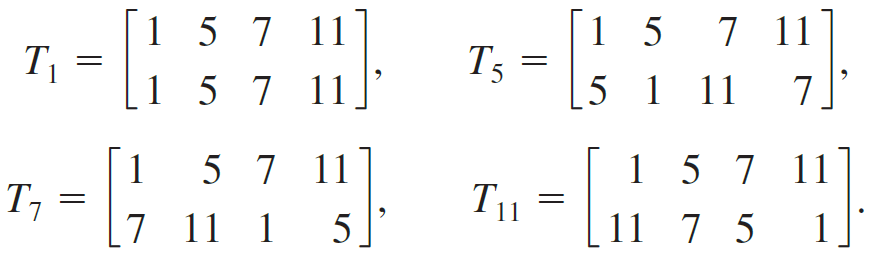
\includegraphics[width=0.6\linewidth]{figures/permutation_U(12).png}
         \caption{The permutations of $U(12)$ in array form.}
         \label{permutation_U(12)}
     \end{figure}
     
     \begin{figure}[!htbp]
         \centering
         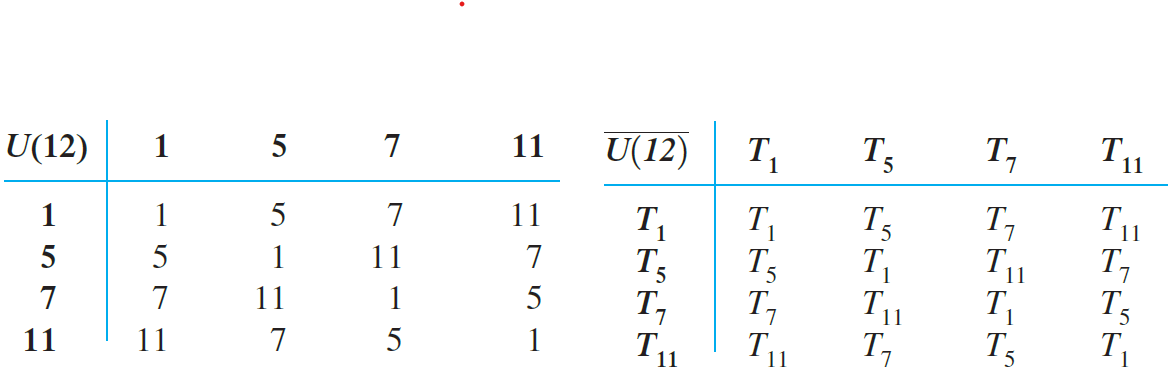
\includegraphics[width=\linewidth]{figures/cayley_table_U(12).png}
         \caption{The Cayley tables for $U(12)$ and $\overline{U(12)}$.}
         \label{cayley_table_U(12)}
     \end{figure}
 \end{example}
 
 \subsection{Properties of Isomorphisms}
 \fbox{\parbox{\linewidth}{
 \begin{theorem}
    Let $\phi: G \to \overline{G}$ be an isomorphism. Then
    \begin{enumerate}[label=(\roman*)]
        \item $e \in G, \overline{e} \in \overline{G}, \phi(e)=\overline{e}$.
        
        \item $\forall n \in \mathbb{Z}, \forall a \in G, \phi(a^n) = (\phi(a))^n$. In additive form, $\phi(na) = n\phi(a)$.
        
        \item $\forall a,b \in G, ab = ba \iff \phi(a)\phi(b) = \phi(b)\phi(a)$.
        
        \item $G = \langle a \rangle \iff \overline{G} = \langle \phi(a) \rangle$.
        
        \item $\forall a \in G, |a| = |\phi(a)|$.
        
        \item $k \in \mathbb{Z}, b \in G, x^k = b$ has the same number of solutions in $G$ as the equation $x^k = \phi(b)$ in $\overline{G}$.
        
        \item If $G$ is finite, then $G$ and $\overline{G}$ have exactly the same number of elements of every order.
    \end{enumerate}
 \end{theorem}
 }}
 
 \begin{proof}
     \begin{enumerate}[label=(\roman*)]
         \item Let $e \in G, \overline{e} \in \overline{G}$. Then,
         \begin{align*}
            \overline{e}\phi(e) &= \phi(ee) = \phi(e)\phi(e), \\
            \overline{e}\phi(e)(\phi(e))^{-1} &= \phi(e)\phi(e)(\phi(e))^{-1}, \\
            \overline{e} &= \phi(e).
         \end{align*}
         
         \item Let $n \in \mathbb{Z}, a \in G$ be arbitrary. Then, 
         \begin{equation*}
             \phi(a^n) = \phi(\underbrace{aa \cdots a}_{n}) = \underbrace{\phi(a)\phi(a)\cdots \phi(a)}_{n} = (\phi(a))^n.
         \end{equation*}
         Hence $\forall n \in \mathbb{Z}, \forall a \in G, \phi(a^n) = (\phi(a))^n$.
         
         \item Let $a,b \in G$ be arbitrary.
         
         $(\Rightarrow)$ Assume that $ab=ba$. Then,
         \begin{equation*}
             ab = ba \implies \phi(ab) = \phi(ba) \implies \phi(a)\phi(b) = \phi(b)\phi(a).
         \end{equation*}
         
         $(\Leftarrow)$ Assume that $\phi(ab) = \phi(ba)$. Then,
         \begin{equation*}
             \phi(ab) = \phi(ba) \implies ab = ba.
         \end{equation*}
         
         \item Let $G = \langle a \rangle$. By closure, $\overline{G} = \langle \phi(a) \rangle$. Since $\phi$ is onto, $\forall b \in \overline{G}, \exists a^k \in G: \phi(a^k) = b$. Then, by Theorem 6.1 (ii),
         \begin{equation*}
             b = \phi(a^k) = (\phi(a))^k \subseteq \langle \phi(a) \rangle. 
         \end{equation*}
         Hence $\overline{G} \subseteq \langle \phi(a) \rangle$ and $\overline{G} = \langle \phi(a) \rangle$.
         
         \item Let $a \in G$ be arbitrary and let $|a|=k$. Then $a^k = e$ and
         \begin{equation*}
             \overline{e} = \phi(e) = \phi(a^k) = (\phi(a))^k.
         \end{equation*}
         So $|\phi(a)| = t \leq k$. Let $t < k$, then
         \begin{equation*}
             \overline{e} = (\phi(a))^t = \phi(a^t) \implies a^t = e.
         \end{equation*}
         But this contradicts that $|a|=k$. Hence $t=k$ and $|a| = |\phi(a)|$.
         
         \item Let $x^k = b \in G, x^k = \phi(b) \in \overline{G}, k \in \mathbb{Z}$. Then,
         \begin{equation*}
             x=b^{1/k} = (\phi(b))^{1/k} = \phi(b^{1/k}). 
         \end{equation*}
         Hence the number of $x: x = b^{1/k} \in G$ is the same as the number of $x: x=\phi(b^{1/k}) \in \overline{G}$.
         
         \item Let $G$ be finite. Since $\phi$ is 1-1 and onto, and by Theorem 6.1 (ii), $\forall a \in G, |a| = |\phi(a)|$. Hence the number of $a \in G: |a| = k$ is the same as the number of $\phi(a) \in \overline{G}: |\phi(a)| = k$.
     \end{enumerate}
 \end{proof}
 
 \fbox{\parbox{\linewidth}{
 \begin{theorem}
    Let $\phi: G \to \overline{G}$ be an isomorphism. Then
    \begin{enumerate}[label=(\roman*)]
        \item $\phi^{-1}: \overline{G} \to G$ is an isomorphism.
        
        \item $G$ is Abelian $\iff$ $\overline{G}$ is Abelian.
        
        \item $G$ is cyclic $\iff \overline{G}$ is cyclic. 
        
        \item $K \leq G \implies \phi(K) = \{\phi(k): k \in K\} \leq \overline{G}$.
        
        \item $\overline{K} \leq \overline{G} \implies \phi^{-1}(\overline{K}) = \{\phi^{-1}(\overline{k}): \overline{k} \in \overline{K}\} \leq G$.
        
        \item For the center $Z(G)$, $\phi(Z(G)) = Z(\overline{G})$.
    \end{enumerate}
 \end{theorem}
 }}
 
 \begin{proof}
     Let $\phi: G \to \overline{G}$ be an isomorphism. Since $\phi:G \to \overline{G}$ is 1-1 and onto, by Theorem 0.6,
         \begin{equation*}
             \exists \phi^{-1}:\overline{G} \to G: \forall g \in G, \phi^{-1}(\phi(g)) = g \text{ and } \forall \overline{g} \in \overline{G}, \phi(\phi^{-1}(\overline{g})) = \overline{g}. 
         \end{equation*}
     \begin{enumerate}[label=(\roman*)]
         \item First, assume that $\forall \overline{a}, \overline{b} \in \overline{G}, \phi^{-1}(\overline{a}) = \phi^{-1}(\overline{b})$, then
         \begin{align*}
             \phi^{-1}(\overline{a}) &= \phi^{-1}(\overline{b}), \\
             \phi(\phi^{-1}(\overline{a})) &= \phi(\phi^{-1}(\overline{b})), \\
             \overline{a} &= \overline{b}.
         \end{align*}
         Hence $\forall \overline{a}, \overline{b} \in \overline{G}, \phi^{-1}(\overline{a}) = \phi^{-1}(\overline{b}) \implies \overline{a} = \overline{b}$. Next, let $a \in G$ be arbitrary, then
         \begin{align*}
             \phi(a) &= \overline{a} \in \overline{G}, \\
             \phi^{-1}(\phi(a)) &= \phi^{-1}(\overline{a}), \\
             a &= \phi^{-1}(\overline{a}).
         \end{align*}
         Hence $\forall a \in G, \exists \overline{a} \in \overline{G}: \phi^{-1}(\overline{a}) = a$. Finally, since $\phi(ab) = \phi(a)\phi(b) = \overline{a}\overline{b}$, it follows that
         \begin{align*}
             \phi^{-1}(\overline{a}\overline{b}) = \phi^{-1}(\phi(ab)) = ab = \phi^{-1}(\overline{a})\phi^{-1}(\overline{b}). 
         \end{align*}
         Hence $\phi^{-1}:\overline{G} \to G$ is an isomorphism.
         
         \item $(\Rightarrow)$ Let $G$ be Abelian. So
         \begin{equation*}
             \forall a,b \in G, ab = ba.
         \end{equation*}
         Then,
         \begin{align*}
             \phi(ab) &= \phi(ba), \\
             \phi(a)\phi(b) &= \phi(b)\phi(a), \\
             \overline{a}\overline{b} &= \overline{b}\overline{a}, \overline{a}, \overline{b} \in \overline{G}.
         \end{align*}
         So $G$ is Abelian $\implies \overline{G}$ is Abelian.
         \\ \\
         $(\Leftarrow)$ Let $\overline{G}$ be Abelian. So
         \begin{equation*}
             \forall \overline{a}, \overline{b} \in \overline{G}, \overline{a}\overline{b} = \overline{b}\overline{a}.
         \end{equation*}
         Then,
         \begin{align*}
             \phi^{-1}(\overline{a}\overline{b}) &= \phi^{-1}(\overline{b}\overline{a}), \\
             \phi^{-1}(\overline{a})\phi^{-1}(\overline{b}) &= \phi^{-1}(\overline{b})\phi^{-1}(\overline{a}), \\
             ab &= ba, a,b \in G.
         \end{align*}
         So $\overline{G}$ is Abelian $\implies G$ is Abelian.
         
         Hence, $G$ is Abelian $\iff \overline{G}$ is Abelian.
         
         \item $(\Rightarrow)$ Let $G$ be cyclic. So $\exists a \in G: G = \langle a \rangle$. Let $\phi(a) = \overline{a} \in \overline{G}$, by closure, $\langle \overline{a} \rangle \subseteq \overline{G}$. Let $\overline{b} \in \overline{G}$, then
         \begin{equation*}
             \exists b \in G: \phi(b) = \overline{b}.
         \end{equation*}
         Since
         \begin{equation*}
             b \in \langle a\rangle \implies b = a^k, k \in \mathbb{Z},
         \end{equation*}
         it follows that
         \begin{equation*}
             \overline{b} = \phi(b) = \phi(a^k) = (\phi(a))^k = \overline{a}^k \in \langle \overline{a} \rangle.
         \end{equation*}
         Hence $\overline{G} \subseteq \langle \overline{a} \rangle$ and $\overline{G} = \langle \overline{a} \rangle$.
         \\ \\
         $(\Leftarrow)$ Let $\overline{G}$ be cyclic. So $\exists \overline{a} \in \overline{G}: G = \langle \overline{a} \rangle$. Let $\phi^{-1}(\overline{a}) = a \in G$, by closure, $\langle a \rangle \subseteq G$. Let $b \in G$, then
         \begin{equation*}
             \exists \overline{b} \in \overline{G}: \phi^{-1}(\overline{b}) = b.
         \end{equation*}
         Since 
         \begin{equation*}
             \overline{b} \in \langle \overline{a} \rangle \implies \overline{b} = \overline{a}^k, k \in \mathbb{Z},
         \end{equation*}
         it follows that
         \begin{equation*}
             b = \phi^{-1}(\overline{b}) = \phi^{-1}(\overline{a}^k) = (\phi^{-1}(\overline{a}))^k = a^k \in \langle a \rangle.
         \end{equation*}
         Hence, $G \subseteq \langle a \rangle$ and $G = \langle a \rangle$.
         
         \item Let $K \leq G$ and $\phi(K) = \{\phi(k): k \in K\} \subseteq \overline{G}$. Since $K \leq G$, 
         \begin{equation*}
             e \in K \implies \phi(e) \in \phi(K).
         \end{equation*}
          Hence $\phi(K) \neq \emptyset$.
          
         Let $a,b \in K$ be arbitrary, then $\phi(a), \phi(b) \in \phi(K)$ and $\phi(a)\phi(b) = \phi(ab)$. Since $K \leq G$, $\forall a,b \in K, ab \in K$. It follows that
         \begin{equation*}
             ab \in K \implies \phi(ab) \in \phi(K).
         \end{equation*}
         Hence $\forall \phi(a),\phi(b) \in \phi(K), \phi(a)\phi(b) \in \phi(K)$.
         
         Let $\phi(a) \in \phi(K)$ be arbitrary. Then $(\phi(a))^{-1} = \phi(a^{-1})$. Since $K \leq G, a \in K \implies a^{-1} \in K$. It follows that
         \begin{equation*}
             a^{-1} \in K \implies \phi(a^{-1}) \in \phi(K).
         \end{equation*}
         Hence $\forall \phi(a) \in \phi(K), (\phi(a))^{-1} \in \phi(K)$.
         
         Hence by Theorem 3.2, $\phi(K) \leq \overline{G}$.
         
         \item Let $\overline{K} \leq \overline{G}$ and $\phi^{-1}(\overline{K}) \in \{\phi^{-1}(\overline{k}): \overline{k} \in \overline{K}\} \subseteq G$. Since $\overline{K} \leq \overline{G}$,
         \begin{equation*}
             \overline{e} \in \overline{K} \implies \phi^{-1}(\overline{e}) \in \phi^{-1}(\overline{K}).
         \end{equation*}
         Hence $\phi(\overline{K}) \neq \emptyset$.
         
         Let $\phi^{-1}(\overline{a}), \phi^{-1}(\overline{b}) \in \phi^{-1}(\overline{K})$ be arbitrary. Then, $\phi^{-1}(\overline{a})\phi^{-1}(\overline{b}) = \phi^{-1}(\overline{a}\overline{b})$. Since $\overline{K} \leq \overline{G}$, it follows that
         \begin{equation*}
             \overline{a}\overline{b} \in \overline{K} \implies \phi^{-1}(\overline{a}\overline{b}) \in \phi^{-1}(\overline{K}).
         \end{equation*}
         Hence $\forall \phi^{-1}(\overline{a}), \phi^{-1}(\overline{b}) \in \phi^{-1}(\overline{K}), \phi^{-1}(\overline{a})\phi^{-1}(\overline{b}) \in \phi^{-1}(\overline{K})$.
         
         Let $\phi^{-1}(\overline{a}) \in \phi^{-1}(\overline{K})$ be arbitrary. Then
         \begin{equation*}
             (\phi^{-1}(\overline{a}))^{-1} = \phi^{-1}(\overline{a}^{-1}).
         \end{equation*}
         Since $\overline{K} \leq \overline{G}$, it follows that $\forall \overline{a} \in \overline{K}, \overline{a}^{-1} \in \overline{K}$, and
         \begin{equation*}
             \overline{a}^{-1} \in \overline{K} \implies \phi^{-1}(\overline{a}^{-1}) \in \phi^{-1}(\overline{K})
         \end{equation*}
         Hence, $\forall \phi^{-1}(\overline{a}) \in \phi^{-1}(\overline{K}), (\phi^{-1}(\overline{a}))^{-1} \in \phi^{-1}(\overline{K})$.
         \\ \\
         Hence by Theorem 3.2, $\phi^{-1}(\overline{K}) \leq G$.
     \end{enumerate}
 \end{proof}
 
 \begin{example}
     Consider $\mathbb{Z}_12, D_6, A_4$. All three groups have order 12. Since the largest order of any element in the three are 12,6,3, respectively, no two are isomorphic. Alternatively, the number of elements of order 2 in each is 1,7,3.
 \end{example}
 
 \begin{example}
     $\mathbb{Q}$ under addition is not isomorphic to $\mathbb{Q}' = \mathbb{Q} \setminus \{0\}$ under multiplication. Because $\forall a \in \mathbb{Q}, a \neq e, |a| = \infty$, since $an = 0 \iff a = 0$, but $|-1|=2$ in $\mathbb{Q}$'.
 \end{example}
 
 \subsection{Automorphisms}
 \fbox{\parbox{\linewidth}{
 \begin{definition}
     An isomorphism $G \approx G$ is an \textit{automorphism} of $G$.
 \end{definition}
 }}
 
 \begin{example}
     The isomorphism $SL(2,\mathbb{R}) \approx SL(2,\mathbb{R})$ in Example 6.6 is an automorphism of $SL(2,\mathbb{R})$.
 \end{example}
 
 \begin{example}
     The function $\phi: \mathbb{C} \to \mathbb{C}$ given by $\phi(a+bi) = a-bi$ is an automorphism of $(\mathbb{C},+)$. The restriction of $\phi$ to $\mathbb{C}$* is an automorphism of ($\mathbb{C}$*,$\cdot$).
 \end{example}
 
 \begin{example}
     Let $\mathbb{R}^2 = \{(a,b): a,b \in \mathbb{R}\}$. Then $\phi(a,b)=(b,a)$ is an automorphism of $\mathbb{R}^2$ under componentwise addition. Geometrically, $\phi$ reflects each point in the plain across the line $y=x$. Generally, any reflection across a line passing through the origin or any rotation of the plane about the origin is an automorphism of $\mathbb{R}^2$.
 \end{example}
 
 \noindent\fbox{\parbox{\linewidth}{
 \begin{definition}
     Let $G$ be a group, and let $a \in G$. The function $\phi_a: \forall x \in G, \phi_a(x) = axa^{-1}$ is the \text{inner automorphism of $G$ induced by $a$.}
 \end{definition}
 }}
 
 \begin{example}
     By Example 6.6, $\phi_a$ is actually an automorphism of $G$.
 \end{example}
 
 \begin{example}
    Figure \ref{example 6.14} shows the inner automorphism of $D_4$ induced by $R_{90}$.
     \begin{figure}
         \centering
         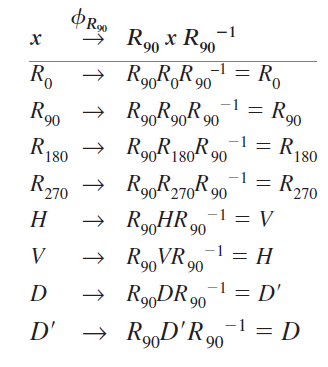
\includegraphics[width=0.4\linewidth]{figures/example6.14.png}
         \caption{}
         \label{example 6.14}
     \end{figure}
 \end{example}
 
 \noindent\fbox{\parbox{\linewidth}{
 \begin{definition}
     $Aut(G)$ is the set of all automorphisms of $G$ and $Inn(G)$ is the set of all inner automorphisms of $G$.
 \end{definition}
 }}
 \\ \\
 \fbox{\parbox{\linewidth}{
 \begin{theorem}
    Let $G$ be a group. Then $Aut(G)$ and $Inn(G)$ are both groups under function composition.
 \end{theorem}
 }}
 
 \begin{proof}
     Let $G$ be a group, and let $Aut(G) = \{\phi:G \to G\ \text{ s.t. } G \approx G\}, Inn(G) = \{\phi_a: a \in G\}$.
     
     WTS $Aut(G)$ is a group. First, let $\phi_1,\phi_2 \in Aut(G), a \in G$ be arbitrary. Then,
     \begin{align*}
         (\phi_1\phi_2)(a) = \phi_1(\phi_2(a)) = \phi_1(b) = c.
     \end{align*}
     Since $\phi_1,\phi_2$ are automorphisms of $G$, it follows that
     \begin{equation*}
         b,c \in G \implies \phi_1\phi_2 \in Aut(G).
     \end{equation*}
     Hence 
     \begin{equation*}
         \forall \phi_1,\phi_2 \in Aut(G), \phi_1\phi_2 \in Aut(G)
     \end{equation*}
     and $Aut(G)$ is closed under function composition. Second, by Theorem 0.6,
     \begin{equation*}
         \forall \phi_1,\phi_2,\phi_3 \in Aut(G), \phi_1(\phi_2\phi_3) = (\phi_1\phi_2)\phi_3.
     \end{equation*}
     Third, let $\phi_e(a) = a, \forall a \in G$. WTS $\phi_e \in Aut(G)$. First, since $\forall a \in G, \phi_e(a) = a$, it follows that $\phi_e: G \to G$. Second, assume that $\forall a,b \in G, \phi_e(a) = \phi_e(b)$. Then,
     \begin{align*}
         \phi_e(a) &= \phi_e(b) \implies a = b.
     \end{align*}
     Hence $\phi_e$ is 1-1. Third, since $\forall a \in G, \exists a \in G: \phi(a) = a$. Hence $\phi_e$ is onto. Finally,
     \begin{align*}
         \phi_e(ab) = ab = \phi_e(a)\phi_e(b).
     \end{align*}
     Hence, $\phi_e$ is an automorphism of $G$ and $\phi_e \in Aut(G)$. It follows that
     \begin{equation*}
         (\phi\phi_e)(a) = \phi(\phi_e(a)) = \phi(a) 
     \end{equation*}
     and
     \begin{equation*}
         (\phi_e\phi)(a) = \phi_e(\phi(a)) = \phi(a).
     \end{equation*}
     Hence,
     \begin{equation*}
         \exists \phi_e \in Aut(G): \forall \phi \in Aut(G), \phi\phi_e = \phi_e\phi = \phi,
     \end{equation*}
     and $\phi_e$ is the identity element of $Aut(G)$. Finally, since $\forall \phi \in Aut(G), \phi:G \to G$ is an automorphism, by Theorem 6.3, $\phi^{-1}: G \to G$ is an isomorphism and $\phi^{-1} \in Aut(G)$. By Theorem 0.6, since $\phi$ is 1-1 and onto,
     \begin{equation*}
         \forall a \in G, (\phi^{-1}\phi)(a) = a = \phi_e(a) \text{ and } (\phi\phi^{-1})(a) = a = \phi_e(a).
     \end{equation*}
     Hence,
     \begin{equation*}
         \forall \phi \in Aut(G), \exists \phi^{-1} \in Aut(G): \phi^{-1}\phi = \phi\phi^{-1} = \phi_e
     \end{equation*}
     and $\phi^{-1}$ is a reverse of $\phi$. Therefore, $Aut(G)$ is a group.
     
     WTS $Inn(G) = \{\phi_a: a\in G\}$ under function composition is a group. First, let $\phi_a,\phi_b \in Inn(G), x \in G$ be arbitrary. Then,
     \begin{align*}
         (\phi_a\phi_b)(x) &= \phi_a(\phi_b(x)) \\
         &= \phi_a(bxb^{-1}), \\
         &= abxb^{-1}a^{-1} \\
         &= (ab)x(ab)^{-1} \quad \text{(Theorem 2.4)}\\
         &= \phi_{ab}(x).
     \end{align*}
     Since $a,b \in G \implies ab \in G$, it follows that $\phi_{ab} \in Inn(G)$ and $Inn(G)$ is closed under function composition. Second, By Theorem 0.6,
     \begin{equation*}
         \phi_a(\phi_b\phi_c) = (\phi_a\phi_b)\phi_c.
     \end{equation*}
     Hence function composition is associative. Third, since $e \in G \implies \phi_e \in Inn(G)$, it follows that
     \begin{equation*}
         (\phi_a\phi_e)(x) = \phi_a(\phi_e(x)) = \phi_a(exe^{-1}) = \phi_a(x)
     \end{equation*}
     and
     \begin{equation*}
         (\phi_e\phi_a)(x) = \phi_e(\phi_a(x)) = \phi_e(axa^{-1}) = eaxa^{-1}e^{-1} = axa^{-1} = \phi_a(x).
     \end{equation*}
     Hence $\phi_a\phi_e = \phi_e\phi_a = \phi_a$ and $\phi_e$ is the identity element of $Inn(G)$. Finally, since $a^{-1} \in G \implies \phi_{a^{-1}} \in Inn(G)$, it follows that
     \begin{align*}
         (\phi_a\phi_{a^{-1}})(x) &= \phi_a(\phi_{a^{-1}}(x)) \\ 
         &= \phi_a(a^{-1}x(a^{-1})^{-1}) \\
         &= \phi_a(a^{-1}xa) \\
         &= aa^{-1}xaa^{-1} \\
         &= x = \phi_e(x)
     \end{align*}
     and
     \begin{align*}
         (\phi_{a^{-1}}\phi_a)(x) &= \phi_{a^{-1}}(\phi_a(x)) \\
         &= \phi_{a^{-1}}(axa^{-1}) \\
         &= a^{-1}axa^{-1}(a^{-1})^{-1} \\
         &= a^{-1}axa^{-1}a \\
         &= x = \phi_e(x).
     \end{align*}
     Hence $\phi_a\phi_{a^{-1}} = \phi_{a^{-1}}\phi_a = \phi_e$ and $\phi_{a^{-1}}$ is the reverse of $\phi_a$. Therefore, $Inn(G)$ is a group under function composition.
 \end{proof}
 
 \begin{example}
     To find $Inn(D_4)$, note that the list of inner automorphisms of $D_4$ is $\{\phi_{R_0}, \phi_{R_{90}}, \phi_{R_{180}}, \phi_{R_{270}}, \phi_H, \phi_V, \phi_D, \phi_{D'}\}$. Since $R_{180} \in Z(D_4) = \{a \in D_4: \forall x \in D_4, ax = xa\}$, it follows that
     \begin{equation*}
         \phi_{R_{180}}(x) = R_{180}xR_{180}^{-1} = x,
     \end{equation*}
     so $\phi_{R_{180}} = \phi_{R_0}$. Also,
     \begin{equation*}
         \phi_{R_{270}}(x) =  R_{270}xR_{270}^{-1} = R_{90}R_{180}xR_{180}^{-1}R_{90}^{-1} = R_{90}xR_{90}^{-1} = \phi_{R_{90}}(x).
     \end{equation*}
     Similarly, since $H=R_{180}V$ and $D'=R_{180}D$, it follows that
     \begin{equation*}
         \phi_H = \phi_V, \phi_D = \phi_{D'}.
     \end{equation*}
     Hence the previous list can be pared down to $\{\phi_{R_0}, \phi_{R_{90}}, \phi_H, \phi_D\}$. WTS these are distinct.
 \end{example}
 
 \begin{example}
     Compute $Aut(\mathbb{Z}_{10})$. Let $\phi \in Aut(\mathbb{Z}_{10}$). Since $\phi$ is an automorphism of $\mathbb{Z}_{10}$, by Theorem 6.2 (ii) and (v),
     \begin{equation*}
        \forall k \in \mathbb{Z}, \phi(k) = k\phi(1)
     \end{equation*}
     and
     \begin{equation*}
         1 \in \mathbb{Z}_{10}, |\phi(1)| = |1| = 10.
     \end{equation*}
     So 
     \begin{equation*}
         \phi \in Aut(\mathbb{Z}_{10}) \implies |\phi(1)| = 10.
     \end{equation*}
     Define
     \begin{equation*}
         \alpha_1(1)=1, \quad \alpha_3(1)=3, \quad \alpha_7(1)=7, \quad \alpha_9(1)=9.
     \end{equation*}
     Since 
     \begin{align*}
         |\alpha_1(1)| = |1| = 10, \\
         |\alpha_3(1)| = |3| = 10, \\
         |\alpha_7(1)| = |7| = 10, \\
         |\alpha_9(1)| = |9| = 10,
     \end{align*}
     it follows that
     \begin{equation*}
         \alpha_1,\alpha_3,\alpha_7,\alpha_9 \in Aut(\mathbb{Z}_{10})
     \end{equation*}
     
     Since
     \begin{align*}
         \forall \phi \in Aut(\mathbb{Z}_{10}), (\alpha_1\phi)(1) = \alpha_1(\phi(1)) = \phi(1)\alpha_1(1) = \phi(1)
     \end{align*}
     and 
     \begin{equation*}
         (\phi\alpha_1)(1) = \phi(\alpha_1(1)) = \phi(1).
     \end{equation*}
     Hence $\alpha_1$ is the identity element of $Aut(\mathbb{Z}_{10})$. Since
     \begin{equation*}
         (\alpha_3\alpha_7)(1) = \alpha_3(\alpha_7(1)) = \alpha_3(7) = 7 \alpha_3(1) = 7\cdot3\bmod10 = 1
     \end{equation*}
     and
     \begin{equation*}
         (\alpha_7\alpha_3)(1) = \alpha_7(\alpha_3(1)) = \alpha_7(3) = 3 \alpha_7(1) = 3\cdot7\bmod10 = 1,
     \end{equation*}
     it follows that $\phi_7$ is the reverse of $\phi_3$ and vice versa. The reverses of $\phi_1$ and $\phi_9$ are themselves. Since
     \begin{align*}
         \alpha_3(1) &= 3, \\
         (\alpha_3\alpha_3)(1) &= (\alpha_3)^2(1) = 3 \cdot 3 \bmod 10 = 9, \\
         (\alpha_3)^3(1) &= 3\cdot3\cdot3\bmod10 = 7, \\
         (\alpha_3)^4(1) &= 3^4\bmod10 = 1, \\
         (\alpha_3)^5(1) &= 3^4\bmod10 = 3, \\
         & \vdots
     \end{align*}
     it follows that $Aut(\mathbb{Z}_{10}) = \langle \alpha_3 \rangle$ and $Aut(\mathbb{Z}_{10})$ is cyclic. Figure \ref{exp6.17} shows that $\mathbb{Z}_{10} \approx U(10)$.
     
     \begin{figure}[!htpb]
         \centering
         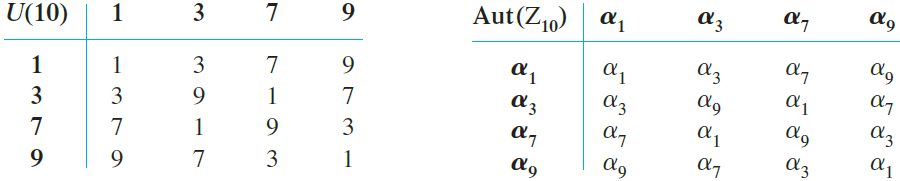
\includegraphics[width=\linewidth]{figures/exp6.17.png}
         \caption{The Cayley tables of $\mathbb{Z}_{10}$ and $U(10)$.}
         \label{exp6.17}
     \end{figure}
 \end{example}

 \noindent\fbox{\parbox{\linewidth}{
 \begin{theorem}
    $\forall n \in \mathbb{N}, Aut(\mathbb{Z}_n) \approx U(n)$.
 \end{theorem}
 }}
 
 \begin{proof}
     (Not covered in lectures) Let $n \in \mathbb{N}$ be arbitrary. Let $\phi \in Aut(\mathbb{Z}_n)$. So $\phi: \mathbb{Z}_n \to \mathbb{Z}_n$ is an automorphism. By Theorem 6.2 (ii),
     \begin{equation*}
        \forall n \in \mathbb{Z}, \phi(n) = n\phi(1).
     \end{equation*}
     Hence any automorphism $\phi$ is determined by the value of $\phi(1)$. By Theorem 6.2 (v),
     \begin{equation*}
         1 \in \mathbb{Z}_n, |\phi(1)| = |1| = n.
     \end{equation*}
     Let $\alpha(1) = 1$, then 
     \begin{equation*}
         |\alpha(1)| = |1| = n \implies \alpha \in \mathbb{Z}_n
     \end{equation*}
     and $\alpha(1) = 1 \in U(n)$. Let $f: Aut(\mathbb{Z}_n) \to U(n)$ such that $f(\phi) = \phi(1)$. 
     
     First, assume that $\forall \alpha, \beta \in Aut(\mathbb{Z}_n), f(\alpha) = f(\beta)$. Then
     \begin{align*}
         f(\alpha) &= f(\beta) \implies \alpha(1) = \beta(1).
     \end{align*}
     It follows that 
     \begin{equation*}
         \forall k \in \mathbb{Z}, \alpha(k) = k\alpha(1) = k\beta(1) = \beta(k).
     \end{equation*}
     Hence $f$ is 1-1. Next, let $b \in U(10)$ be arbitrary and let $\alpha(a) = ab \bmod n, \forall a \in \mathbb{Z}_n$. $\alpha$ is an automorphism of $\mathbb{Z}_n$ and $\alpha \in Aut(\mathbb{Z}_n)$. Since
     \begin{equation*}
         f(\alpha) = \alpha(1) = 1\cdot b \bmod n = b \in U(n),
     \end{equation*}
     $f$ is onto. Finally, since
     \begin{align*}
         f(\alpha\beta) &= (\alpha\beta)(1) \\
         &= \alpha(\beta(1)) \\
         &= \beta(1)\alpha(1) \\
         &= \alpha(1)\beta(1) \\
         &= f(\alpha)f(\beta).
     \end{align*}
     Hence $Aut(\mathbb{Z}_n) \approx U(n)$. 
 \end{proof}
 
 \begin{example}
     Consider $H \leq S_4$,
     \begin{equation*}
         H = \{(1),(1234),(13)(24),(1432),(12)(34),(24),(14)(23),(13)\}.
     \end{equation*}
     One has the subgroups
     \begin{equation*}
         (12)H(21) = \{(1),(1342),(14)(23),(1234),(12)(34),(14),(13)(24),(23)\}
     \end{equation*}
     and
     \begin{equation*}
         (123)H(321) = \{(1),(1423),(12)(34),(1324),(14)(23),(34),(13)(24),(12)\}
     \end{equation*}
     of $S_4$ that are isomorphic to $H$.
 \end{example}
 
  \section{Cosets and Lagrange's Theorem}
 \subsection{Properties of Cosets}
 \fbox{\parbox{\linewidth}{
 \begin{definition}
     Let $G$ be a group and let $H \leq G, H \neq \emptyset$. For any $a \in G$,
     \begin{equation*}
         aH = \{ah: h \in H\}, \quad Ha = \{ha: h \in H\}, \quad aHa^{-1} = \{aha^{-1}: h \in H\}. 
     \end{equation*}
     The set $aH$ is the \textit{left coset of $H$ in $G$ containing $a$}, $Ha$ is the \textit{right coset of $H$ in $G$ containing $a$}. The element $a$ is the \textit{coset representative of $aH$ or $Ha$. The number of elements in $aH$ is $|aH|$, and the number of elements in $Ha$ is $|Ha|$.}
 \end{definition}
 }}
 
 \begin{example}
     Let $G=S_3$ and $H=\{(1),(13)\}$. Then the left cosets of $H$ in $G$ are
     \begin{align*}
         (1)H &= H, \\
         (12)H &= \{(12),(12)(13)\} = \{(12),(132)\} = (132)H, \\
         (13)H &= \{(13),(1)\} = H, \\
         (23)H &= \{(23),(23)(13)\} = \{(23),(123)\} = (123)H.
     \end{align*}
  \end{example}

     \begin{example}
         Let $\alpha=\{R_0,R_{180}\} \leq D_4$. Then
         \begin{align*}
             R_0\alpha &= \alpha, \\
             R_{90}\alpha &= \{R_{90},R_{270}\} = R_{270}\alpha, \\
             R_{180}\alpha &= \{R_{180},R_0\} = \alpha, \\
             V\alpha &= \{V,H\} = H\alpha, \\
             D\alpha &= \{D,D'\} = D\alpha.
         \end{align*}
     \end{example}
     
     \begin{example}
         Let $H = \{0,3,6\} \leq \mathbb{Z}_9$ under addition. Then the left cosets of $H$ in $\mathbb{Z}_9$ are
         \begin{align*}
             0+H &= \{0+0,0+3,0+6\} = \{0,3,6\} = 3+H = 6+H, \\
             1+H &= \{1,4,7\} = 4+H = 7+H, \\
             2+H &= \{2,5,8\} = 5+H = 8+H.
         \end{align*}
     \end{example}
     
     \noindent\fbox{\parbox{\linewidth}{
     \begin{lemma}
         Let $G$ be a group, $H \leq G$, and $a,b \in G$. Then,
         \begin{enumerate}[label=(\roman*)]
             \item $a \in aH$.
             \item $aH = H \iff a \in H$.
             \item $(ab)H = a(bH)$ and $H(ab) = (Ha)b$.
             \item $aH=bH \iff a \in bH$.
             \item $(aH=bH)$ or $(aH \cap bH = \emptyset)$,
             \item $aH=bH \iff a^{-1}b \in H$.
             \item $|aH|=|bH|$.
             \item $aH=Ha \iff H=aHa^{-1}$.
             \item $aH \leq G \iff a \in H$.
         \end{enumerate}
     \end{lemma}
     }}
     
     \begin{proof}
     Let $G$ be a group, $H \leq G$, and $a,b \in G$.
         \begin{enumerate}[label=(\roman*)]
             \item Since $e \in H$, it follows that $a = ae \in aH$.
             
             \item $(\Rightarrow)$ Assume that $aH = H$. Then by Lemma 7.1 (i),
             \begin{equation*}
                 a \in aH = H.
             \end{equation*}
             
             $(\Leftarrow)$ Assume that $a \in H$. Let $ah \in aH$, then
             \begin{equation*}
                 a \in H, h \in H \implies ah \in H.
             \end{equation*}
             Let $h \in H$. Since
             \begin{equation*}
                 a \in H \implies a^{-1} \in H,
             \end{equation*}
             it follows that $a^{-1}h \in H$. Then
             \begin{equation*}
                 h = eh = (aa^{-1})h = a(a^{-1}h) \in aH.
             \end{equation*}
             
             \item Let $(ab)h \in (ab)H$. Then
             \begin{equation*}
                 (ab)h = a(bh) \in a(bH) \implies (ab)H \subseteq a(bH).
             \end{equation*}
             Let $a(bh) \in a(bH)$. Then
             \begin{equation*}
                 a(bh) = (ab)h \in (ab)H \implies a(bH) \subseteq (ab)H.
             \end{equation*}
             Hence $(ab)H = a(bH)$.
             
             Let $h(ab) \in H(ab)$. Then
             \begin{equation*}
                 h(ab) = (ha)b \in (Ha)b \implies H(ab) \subseteq (Ha)b.
             \end{equation*}
             Let $(ha)b \in (Ha)b$. Then
             \begin{equation*}
                 (ha)b = h(ab) \in H(ab) \implies (Ha)b \subseteq H(ab).
             \end{equation*}
             Hence $H(ab)=(Ha)b$.
             
             \item $(\Rightarrow)$ Assume that $aH=bH$. Then
             \begin{equation*}
                 a = ae \in aH = bH.
             \end{equation*}
             $(\Leftarrow)$ Assume that $a \in bH$. Then $a = bh$ and by Lemma 7.1 (iii),
             \begin{equation*}
                 aH = (bh)H = b(hH).
             \end{equation*}
             Since $h \in H$, by Lemma 7.1 (ii), $hH = H$ and hence
             \begin{equation*}
                 aH = b(hH) = bH.
             \end{equation*}
             
             \item Assume that $aH = bH$. Then 
             \begin{equation*}
                 aH \cap bH = aH = bH \neq \emptyset.
             \end{equation*}
             Assume that $aH \cap bH = \emptyset$. Then
             \begin{equation*}
                 \neg (\exists x: x \in aH, x \in bH) \implies aH \neq bH.
             \end{equation*}
             
             \item $(\Rightarrow)$ Assume that $aH=bH$. Since
             \begin{align*}
                 a(a^{-1}bH) &= b(a^{-1}bH), \\
                 bH &= ba^{-1}bH, \\
                 H &= a^{-1}bH, \\
                 aH &= bH,
             \end{align*}
             it follows that
             \begin{equation*}
                 aH = bH \iff a^{-1}bH = H.
             \end{equation*}
             By Lemma 7.1 (ii),
             \begin{equation*}
                 a^{-1}bH = H \iff a^{-1}b \in H.
             \end{equation*}
             $(\Leftarrow)$ Assume that $a^{-1}b \in H$. Then
             \begin{align*}
                 a^{-1}bH = H \implies bH = aH.
             \end{align*}
             
             \item Since $|aH| = |H|, |bH| = |H|$, it follows that $|aH| = |bH|$.
             
             \item $(\Rightarrow)$ Assume that $aH=Ha$. Then
             \begin{align*}
                 aH &= Ha, \\
                 aHa^{-1} &= H.
             \end{align*}
             $(\Leftarrow)$ Assume that $H=aHa^{-1}$. Then
             \begin{align*}
                 H &= aHa^{-1}, \\
                 Ha &= aH.
             \end{align*}
             
             \item $(\Rightarrow)$ Assume that $aH \leq G$. Then
             \begin{equation*}
                e \in aH, e = ee \in eH \implies aH \cap eH \neq \emptyset.
             \end{equation*}
             By Lemma 7.1 (v), $aH = eH = H$. By Lemma 7.1 (ii),
             \begin{equation*}
                 aH=H \iff a \in H.
             \end{equation*}
             $(\Leftarrow)$ Assume that $a \in H$. By Lemma 7.1 (ii),
             \begin{equation*}
                 a \in H \iff aH = H \leq G.
             \end{equation*}
         \end{enumerate}
     \end{proof}
     
     \begin{example}
         Find the cosets of $H = \{1,15\}$ in $G = U(32) = \{1,3,5,7,9,11,13,15,17,19, \\ 21,23,25,27,29,31\}$.
         
         \begin{align*}
             1H &= \{1,15\} = 15H, \\
             3H &= \{3,13\} = 13H, \\
             5H &= \{5,11\} = 11H, \\
             7H &= \{7,9\} = 9H, \\
             17H &= \{17, 31\} = 31H, \\
             19H &= \{19, 29\} = 29H, \\
             21H &= \{21, 27\} = 27H, \\
             23H &= \{23, 25\} = 25H. \\
         \end{align*}
     \end{example}
     
     \subsection{Lagrange's Theorem and Consequences}
     \fbox{\parbox{\linewidth}{
     \begin{theorem}[Lagrange's Theorem]
        Let $G$ be a group, $|G|=n$. Then
        \begin{equation*}
            H \leq G \implies |H| \mid |G|.
        \end{equation*}
        Moreover, the number of distinct left and right cosets of $H$ in $G$ is $|G|/|H|$.
     \end{theorem}
     }}
     
     \begin{proof}
        Let $G$ be a group, $|G|=n$. Assume that $H \leq G$. Let $a_1H,a_2H,\dots,a_rH$ be the distinct left cosets of $H$ in $G$. Then,
        \begin{equation*}
            \forall a \in G, \exists i \in \{1,2,\dots,r\}: aH = a_iH.
        \end{equation*}
        By Lemma 7.1 (i), $a \in aH$. So 
        \begin{equation*}
            \forall a \in G, \exists i \in \{1,2,\dots,r\}: a \in a_iH.
        \end{equation*}
        It follows that
        \begin{equation*}
            G = a_1H \cup \dots \cup a_rH.
        \end{equation*}
        By Lemma 7.1 (v), this union is disjoint, so
        \begin{equation*}
            |G| = |a_1H| + |a_2H| + \dots + |a_rH|.
        \end{equation*}
        Since 
        \begin{equation*}
            \forall i \in \{1,\dots, r\}, |a_iH| = |H|,
        \end{equation*}
        it follows that 
        \begin{align*}
            |G| &= |a_1H| + |a_2H| + \dots + |a_rH| \\
            &= \underbrace{|H|+\dots+|H|}_{r} \\
            &= r|H|.
        \end{align*}
        Hence $|H| \mid |G|$ and the number of distinct left and right cosets of $H$ in $G$ is $r=|G|/|H|$.
     \end{proof}
     
     \noindent\fbox{\parbox{\linewidth}{
     \begin{definition}
         The \textit{index} of $H \leq G$, denoted by $|G:H|$, is the number of distinct left cosets of $H$ in $G$.
     \end{definition}
     }}
     \\ \\
     \fbox{\parbox{\linewidth}{
     \begin{corollary}
             $|G|=n,H \leq G \implies |G:H| = |G|/|H|.$
     \end{corollary}
     }}
     \\ \\
     \fbox{\parbox{\linewidth}{
     \begin{corollary}
             $|G| = n \implies \forall a \in G, |a| \mid |G|$.
     \end{corollary}
     }}
     
     \begin{proof}
        Let $G$ be a group and $|G|=n$. Let $a \in G$ be arbitrary. By Theorem 3.4, $\langle a \rangle \leq G$. By Theorem 7.1, $|\langle a \rangle| \mid |G|$. Hence
        \begin{equation*}
            \forall a \in G, |a| \mid |G|.
        \end{equation*}
     \end{proof}
     
     \noindent\fbox{\parbox{\linewidth}{
     \begin{corollary}
             $|G|=p, p \text{ is prime} \implies G \text{ is cyclic.}$
     \end{corollary}
     }}
     
     \begin{proof}
        Let $G$ be a group and $|G| = p$, $p$ is prime. Let $a \in G$ and $a \neq e$. Then, by Theorem 3.4, $\langle a \rangle \leq G$. By Theorem 7.1, $|\langle a \rangle| \mid |G|$. Since $|G|=p$, it follows that $|\langle a \rangle| \in \{1,p\}$. But 
        \begin{equation*}
            a \neq e \implies \langle a \rangle \neq 1.
        \end{equation*}
        Hence 
        \begin{equation*}
            |\langle a \rangle| = p = |G|, \langle a \rangle \leq G \implies G = \langle a \rangle.
        \end{equation*}
     \end{proof}
     
     \noindent\fbox{\parbox{\linewidth}{
     \begin{corollary}
             $|G|=n,a \in G \implies a^{|G|}=e$.
     \end{corollary}
     }}
     
     \begin{proof}
        Let $G$ be a group, $|G|=n$, and $a \in G$. By Corollary 7.1.2, $|a| \mid |G|$, so $|G| = |a|k, k \in \mathbb{Z}$. Then
        \begin{equation*}
            a^{|G|} = a^{|a|k} = e^k = e.
        \end{equation*}
     \end{proof}
     
     \noindent\fbox{\parbox{\linewidth}{
     \begin{corollary}[Fermat's Little Theorem]
             $\forall a \in \mathbb{Z}, \forall p = \text{prime}, a^p \bmod p = a \bmod p$.
     \end{corollary}
     }}
     
     \begin{proof}
        Let $a \in \mathbb{Z}$ and $p$ is prime. By the division algorithm,
        \begin{equation*}
            a = pm + r, 0 \leq r < p.
        \end{equation*}
        So $a \bmod p = r$. If $r = 0$, then $a \bmod p = 0$ and $a^p \bmod p = 0$. If $0 < r < p$, let $r \in U(p) = \{1,2,\dots,p-1\}$ under multiplication modulo $p$. Then by Corollary 7.1.4, 
        \begin{equation*}
            r^{|U(p)|} = r^{p-1} = 1.
        \end{equation*}
        It follows that
        \begin{equation*}
            r^{p-1} \bmod p = 1 \implies r^p \bmod p = r.
        \end{equation*}
     \end{proof}
     
     \begin{example}
         The converse of Lagrange's Theorem is false. By Table 5.1, $A_4$ has eight elements of order 3 ($\alpha_5$ through $\alpha_{12}$). Let $H \leq A_6, |H| = 6$. Let $a \in A_4, |a| = 3$. By Theorem 7.1, 
         \begin{equation*}
            |A_4:H|=|A_4|/|H|=12/6=2.
         \end{equation*}
         So at most two of the cosets $H, aH, a^2H$ are distinct. But equality of any pair of these three implies that $aH = H \implies a \in H$. Thus, $H: |H|=6$ would have to contain all eight $a \in A_4, |a|=3$, which is absurd.
     \end{example}
     
     \noindent\fbox{\parbox{\linewidth}{
     \begin{theorem}
        Let $G$ be a group, $H,K \leq G$, $|H|=m, |K|=n$. Define the set $HK = \{hk: h \in H, k \in K\}$. Then $|HK| = |H||K|/|H \cap K|$.
     \end{theorem}
     }}
     
     \begin{proof}
        Although the set $HK$ has $|H||K|$ products, there may be $hk = h'k', h \neq h', k \neq k'$. For every $t \in H \cap K$, the product $hk = (ht)(t^{-1}k)$, so each element in $HK$ is represented by at least $|H\cap K|$ products in $HK$. But
        \begin{equation*}
            hk = h'k' \implies t = h^{-1}h' = kk'^{-1} \in H \cap K \implies h' = ht, k' = t^{-1}k.
        \end{equation*}
        Thus each element in $HK$ is represented by exactly $|H \cap K|$ products. So $|HK| = |H||K|/|H \cap K|$.
     \end{proof}
     
     \begin{example}
         A group of order 75 can have at most one subgroup of order 25. Suppose $H, K$ are two subgroups of order 25. Since 
         \begin{equation*}
             |H \cap K| \mid |H| = |H \cap K| \mid 25 \implies |H \cap K| \in \{1,5\}.
         \end{equation*}
         It follows that
         \begin{equation*}
             |HK| = |H||K|/|H \cap K| = 25\cdot25/|H\cap K| \in \{625,125\}.
         \end{equation*}
         Hence
         \begin{equation*}
             |H \cap K| = 25 \implies H=K.
         \end{equation*}
     \end{example}
     
     \noindent\fbox{\parbox{\linewidth}{
     \begin{theorem}
        Let $G$ be a group and $p>2$ is a prime. Then
        \begin{equation*}
            |G|=2p \implies G \approx \mathbb{Z}_{2p} \text{ or } G \approx D_p.
        \end{equation*}
     \end{theorem}
     }}
     
     \begin{proof}
        Let $G$ be a group and $p>2$ is a prime. Let $|G|=2p$. Assume that $\forall a \in G, |a| \neq 2p$. Since $a \in G, a \neq e, \langle a \rangle \leq G$, by the Lagrange's Theorem, 
        \begin{equation*}
            |G|=2p, \langle a \rangle \leq G \implies |\langle a \rangle| \mid |G| \implies |a| \mid 2p.
        \end{equation*}
        Hence
        \begin{equation*}
            \forall a \in G, a \neq e, |a| = 2 \text{ or } |a| = p.
        \end{equation*}
        If $|a|=2$, then
        \begin{equation*}
            \forall a, b \in G, ab = (ab)^{-1} = b^{-1}a^{-1} = ba.
        \end{equation*}
        So $G$ is Abelian. Then, $\forall a, b \in G, a,b \neq e, a \neq b$, the set $\{e,a,b,ab\}$ is closed and hence is a subgroup of $G$ of order 4. But this contradicts the Lagrange's Theorem since
        \begin{equation*}
            |G|=2p, H \leq G \implies |H| \mid |G| = 2p,
        \end{equation*}
        and 4 does not divide $2p$. Hence $|a| = p$.
        
        Let $b \in G: b \neq \langle a \rangle$ be arbitrary. Then by the Lagrange's Theorem and the assumption that $\forall a \in G, |a| \neq 2p$, one has $|b|=2$ or $|b|=p$. Since $\langle a 
        \rangle, \langle b \rangle \leq G, |\langle a \rangle| \neq \infty, |\langle b \rangle| \neq \infty$, by Theorem 7.2, 
        \begin{equation*}
            |\langle a \rangle \cap \langle b \rangle| \mid |\langle a \rangle| = |a| = p.
        \end{equation*}
        So $|\langle a \rangle \cap \langle b \rangle| = 1$ or $|\langle a \rangle \cap \langle b \rangle| = p$. Since $\langle a \rangle \neq \langle b \rangle$ and $e \in \langle a \rangle, e \in \langle b \rangle$, it follows that $|\langle a \rangle \cap \langle b \rangle| = 1$. If $|b| = p$, then by Theorem 7.2,
        \begin{equation*}
            |\langle a \rangle \langle b \rangle| = |\langle a \rangle||\langle b \rangle| = p^2 > 2p = |G|,
        \end{equation*}
        which is impossible. Hence $\forall b \in G, b \notin \langle a \rangle, |b| = 2$.
        
        Consider $ab$. Since $ab \notin \langle a \rangle$, $|ab| = 2$. Then
        \begin{equation*}
            ab = (ab)^{-1} = b^{-1}a^{-1} = ba^{-1}.
        \end{equation*}
        This relation completel determines the multiplication table for $G$. For example,
        \begin{align*}
            a^3(ba^4) &= a^2(ab)a^4 \\ 
            &= a^2(ba^{-1})a^4 \\
            &= a(ab)a^3 \\
            &= a(ba^{-1})a^3 \\
            &= (ab)a^2 \\
            &= (ba^{-1})a^2 \\ 
            &= ba.
        \end{align*}
        Since the multiplication table for all noncclic groups of order $2p$ is uniquely determined by the relation $ab=ba^{-1}$, all noncyclic groups of order 2p must be isomorphic to each other. 
     \end{proof}
     
     \subsection{An Application of Cosets to Permutation Groups}
     \fbox{\parbox{\linewidth}{
     \begin{definition}
         Let $G$ be a group of permutation of a set $S$. The \textit{stabilizer of $i \in S$ in $G$ is 
         \begin{equation*}
             stab_G(i) = \{\phi \in G: \phi(i) = i\}.
         \end{equation*}}
     \end{definition}
     }}
     \\ \\
     Proof that $stab_G(i) \leq G$. Let $G$ be a group of permutation of a set $S$, let
     \begin{equation*}
         stab_G(i) = \{\phi \in G: \phi(i) = i\}, i \in S.
     \end{equation*}
     Let $\phi_1,\phi_2 \in stab_G(i)$, so $\phi_1(i)=i,\phi_2(i)=i$. It follows that
     \begin{equation*}
         (\phi_1\phi_2)(i) = \phi_1(\phi_2(i)) = \phi_1(i) = i \implies \phi_1\phi_2 \in stab_G(i).
     \end{equation*}
     Let $\phi \in stab_G(i)$. Then
     \begin{equation*}
         \phi(\phi^{-1}(i)) = (\phi\phi^{-1})(i) = \epsilon(i) = i \implies \phi^{-1}(i) = i.
     \end{equation*}
     It follows that $\phi^{-1} \in stab_G(i)$. Hence by the Two-step Subgroup Test, $stab_G(i) \leq G$.
     \\ \\
     \fbox{\parbox{\linewidth}{
     \begin{definition}
         Let $G$ be a group of permutations of a set $S$. The \textit{orbit of $i \in S$ under $G$} is
         \begin{equation*}
             orb_G(i) = \{\phi(i): \phi \in G\}.
         \end{equation*}
         The number of elements in $orb_G(i)$ is $|orb_G(i)|$.
     \end{definition}
     }}
     
     \begin{example}
         Let
         \begin{align*}
             G = \{(1),(132)(456)(78),(132)(465),(123)(456),(123)(456)(78),(78)\} \leq S_8.
         \end{align*}
         Then,
         \begin{align*}
             orb_G(1) &= \{1,3,2\}, & stab_G(1) &= \{(1),(78)\}, \\
             orb_G(2) &= \{2,1,3\}, & stab_G(2) &= \{(1),(78)\}, \\
             orb_G(4) &= \{4,6,5\}, & stab_G(4) &= \{(1),(78)\}, \\
             orb_G(7) &= \{7,8\}, & stab_G(7) &= \{(1),(132)(465),(123)(456)\}.
         \end{align*}
     \end{example}
     
     \begin{example}
         Let $D_4$ be a group of permutation of a square. Figure \ref{D_4}(a) and (b) show $orb_{D_4}(p)$ and $orb_{D_4}(q)$, respectively. Furthermore, $stab_{D_4}(p) = \{R_0,D\}$ and $stab_{D_4}(q)=\{R_0\}$.
         
         \begin{figure}[!htbp]
             \centering
             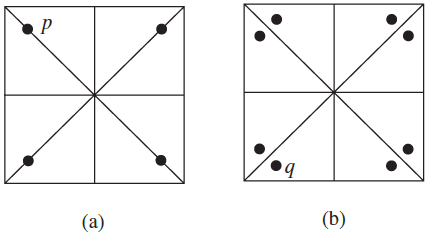
\includegraphics[width=0.6\linewidth]{figures/exp7.8.png}
             \caption{(a) $orb_{D_4}(p)$. (b) $orb_{D_4}(q)$.}
             \label{D_4}
         \end{figure}
     \end{example}
     
     \noindent\fbox{\parbox{\linewidth}{
     \begin{theorem}[Orbit-Stabilizer Theorem]
        Let $G$ be a finite group of permutations of a set $S$. Then,
        \begin{equation*}
            i \in S, |G| = |orb_G(i)||stab_G(i)|.
        \end{equation*}
     \end{theorem}
     }}
     
     \begin{proof}
        Let $G$ be a group of permutation of a set $S$ and $|G|=n$. By the Lagrange Theorem,
        \begin{equation*}
            stab_G(i) \leq G \implies |stab_G(i)| \mid G, i \in S
        \end{equation*}
        and the number of distinct left cosets of $stab_G(i)$ in $G$, $r = |G|/|stab_G(i)|$.
        \\ \\
        Let
        \begin{equation*}
            T: \{\phi stab_G(i): \phi \in G\} \to orb_G(i) = \{\phi(i): \phi \in G\}.
        \end{equation*}
        Assume that $\alpha stab_G(i) = \beta stab_G(i)$. Then by Lemma 7.1,
        \begin{equation*}
            \alpha stab_G(i) = \beta stab_G(i) \iff \alpha^{-1}\beta \in stab_G(i).
        \end{equation*}
        It follows that
        \begin{equation*}
            (\alpha^{-1}\beta)(i) = i \implies \alpha(i) = \alpha(\alpha^{-1}\beta(i)) = (\alpha\alpha^{-1}\beta)(i) = \beta(i).
        \end{equation*}
        Hence $T$ is a well-defined function. 
        \\ \\
        Assume that $\alpha(i) = \beta(i)$. Then $(\alpha^{-1}\beta)(i) = i$ and it follows that by Lemma 7.1,
        \begin{equation*}
            \alpha stab_G(i) = \beta stab_G(i) \iff \alpha^{-1}\beta \in stab_G(i).
        \end{equation*}
        Hence $T$ is 1-1. Let $j \in orb_G(i)$ be arbitrary. Since
        \begin{equation*}
            \exists \alpha \in G: \alpha(i) = j,
        \end{equation*}
        it follows that
        \begin{equation*}
            T(\alpha stab_G(i)) = \alpha(i) = j.
        \end{equation*}
        Hence $T$ is onto $orb_G(i)$. Thus, 
        \begin{equation*}
            |orb_G(i)| = r = |G|/|stab_G(i)| \implies |G| = |orb_G(i)||stab_G(i)|.
        \end{equation*}
     \end{proof}
     
     \subsection{The Rotation Group of a Cube and a Soccer Ball}
     \fbox{\parbox{\linewidth}{
     \begin{theorem}
        The group of rotations of a cube is isomorphic to $S_4$.
     \end{theorem}
     }}
     
     \begin{proof}
        
     \end{proof}
     
     \section{External Direct Products}
     \subsection{Definition and Examples}
     \fbox{\parbox{\linewidth}{
     \begin{definition}
         Let $G_1,G_,\dots,G_n$ be a finite collection of groups. The \textit{external direct product} of $G_1,G_2,\dots,G_n$ is
         \begin{equation*}
             G_1 \oplus G_2 \oplus \cdots \oplus G_n = \{(g_1,g_2,\dots,g_n): g_i \in G_i\},
         \end{equation*}
         where
         \begin{equation*}
             (g_1,g_2,\dots,g_n)(g_1',g_2',\dots,g_b') = (g_1g_1',g_2g_2',\dots,g_ng_n').
         \end{equation*}
         Each $g_ig_i'$ is performed with the operation of $G_i$. If each $G_i$ is finite, then
         \begin{equation*}
             |G_1 \oplus G_2 \oplus \cdots \oplus G_n| = |G_1||G_2|\cdots|G_n|.
         \end{equation*}
     \end{definition}
     }}
     \\ \\
     Proof that $G_1 \oplus \cdots \oplus G_n$ is  a group. Since
     \begin{equation*}
         (g_1,\dots,g_n)(g_1',\dots,g_n') = (g_1g_1',\dots,g_ng_n')
     \end{equation*}
     and $g_1g_1' \in G_1, \dots, g_ng_n' \in G_n$, it follows that $G_1 \oplus \cdots \oplus G_n$ is closed. Next, since
     \begin{align*}
         [(g_1,\dots,g_n)(g_1',\dots,g_n')](g_1'',\dots,g_n'') &= (g_1g_1',\dots,g_ng_n')(g_1'',\dots,g_n'') \\
         &= [(g_1g_1')g_1'',\dots,(g_ng_n')g_n''] \\
         &= [g_1(g_1'g_1''),\dots,g_n(g_n'g_n'')] \\
         &= (g_1,\dots,g_n)(g_1'g_1'',\dots,g_n'g_n'') \\
         &= (g_1,\dots,g_n)[(g_1',\dots,g_n')(g_1'',\dots,g_n'')],
     \end{align*}
     it follows that $G_1 \oplus \cdots \oplus G_n$ is associative. Further, since
     \begin{align*}
         (e_1,\dots,e_n)(g_1,\dots,g_n) &= (e_1g_1,\dots,e_ng_n) \\
         &= (g_1,\dots,g_n) \\
         &= (g_1e_1,\dots,g_ne_n) \\
         &= (g_1,\dots,g_n)(e_1,\dots,e_n),
     \end{align*}
     it follows that $(e_1,\dots,e_n)$ is the identity element of $G_1 \oplus \cdots \oplus G_n$. Lastly, since
     \begin{align*}
         (g_1^{-1},\dots,g_n^{-1})(g_1,\dots,g_n) &= (g_1^{-1}g_1,\dots,g_n^{-1}g_n) \\
         &= (e_1,\dots,e_n) \\
         &= (g_1g_1^{-1},\dots,g_ng_n^{-1}) \\
         &= (g_1,\dots,g_n)(g_1^{-1},\dots,g_n^{-1}),
     \end{align*}
     it follows that $(g_1^{-1},\dots,g_n^{-1})$ is the reverse of $(g_1,\dots,g_n)$. Hence, $G_1 \oplus \cdots \oplus G_n$ is a group. 
     
     \begin{example}
     Consider $U(8) = \{1,3,5,7\}, U(10) = \{1,3,7,9\}$. Then
         \begin{align*}
             U(8) \oplus U(10) = \{(1,1),(1,3),(1,7),(1,9), \\ (3,1)(3,3), (3,7),(3,9), \\ (5,1),(5,3)(5,7),(5,9), \\ (7,1),(7,3),(7,7),(7,9)\}.
         \end{align*}
         The product $(3,7)(7,9) = (3\cdot7 \bmod 8, 7\cdot9 \bmod 10) = (5,3)$.
     \end{example}
     
     \begin{example}
     Consider $\mathbb{Z}_2 = \{0,1\}$ and $\mathbb{Z}_3=\{0,1,2\}$. Then
     \begin{equation*}
         \mathbb{Z}_2 \oplus \mathbb{Z}_3 = \{(0,0),(0,1),(0,2),(1,0),(1,1),(1,2)\}.
     \end{equation*}
     Since
     \begin{align*}
         (0,0)(0,1) &= (0,1) = (0,1)(0,0), \\
         (0,0)(0,2) &= (0,2) = (0,2)(0,0), \\
         & \vdots \\
         (1,1)(1,2) &= (0,0) = (1,2)(1,1),
     \end{align*}
     it follows that $\mathbb{Z}_2 \oplus \mathbb{Z}_3$ is an Abelian group of order 6. Since the operation in each component is addition,
     \begin{align*}
         (1,1) &= (1,1), \\
         2(1,1) &= (0,2), \\
         3(1,1) &= (1,0), \\
         4(1,1) &= (0,1), \\
         5(1,1) &= (1,2), \\
         6(1,1) &= (0,0).
     \end{align*}
     Hence $\mathbb{Z}_2 \oplus \mathbb{Z}_3 = \langle (1,1) \rangle$. It follows that $\mathbb{Z}_2 \oplus \mathbb{Z}_3 \approx \mathbb{Z}_6$.
     \end{example}
     
     \begin{example}
     Let $G$ be a group of order 4. By the Lagrange's Theorem,
     \begin{equation*}
         |G| = 4, \langle a \rangle \leq G, a \in G \implies |\langle a \rangle| = |a| \mid |G| = 4.
     \end{equation*}
     So $a \in G, a \in \{1,2\}$. Let $a,b \in G, a \neq e, b \neq e, a \neq b$. Then, $ab \neq a, ab \neq b$, and $ab \neq e$, otherwise $a = b^{-1} = b$. Thus $G = \{e,a,b,ab\}$. Since $ab = (ab)^{-1} = b^{-1}a^{-1} = ba$, the operation table is uniquely determined. Hence $G \approx \mathbb{Z}_4$ or $G \approx \mathbb{Z}_2 \oplus \mathbb{Z}_2$.
     \end{example}
     
     \subsection{Properties of External Direct Products}
     \fbox{\parbox{\linewidth}{
     \begin{theorem}
        $|(g_1,g_2,\dots,g_n)| = \lcm(|g_1|,|g_2|,\dots,|g_n|)$.
     \end{theorem}
     }}
     
     \begin{proof}
        Let $s = \lcm(|g_1|,|g_2|,\dots,|g_n|)$ and $t = |(g_1,g_2,\dots,g_n)|$. Since $s$ is a multiple of each $|g_i|$, by Theorem 4.1 (ii),
        \begin{equation*}
            g_i^s = g_i^0 = e_i \iff |g_i| \mid (s-0) = s.
        \end{equation*}
        It follows that
        \begin{equation*}
            (g_1,g_2,\dots,g_n)^s = (g_1^s,g_2^s,\dots,g_n^s) = (e_1,e_2,\dots,e_n)
        \end{equation*}
        and $t \leq s$. On the other hand, since
        \begin{equation*}
            (e_1,e_2,\dots,e_n) = 
            (g_1,g_2,\dots,g_n)^t =
            (g_1^t,g_2^t,\dots,g_n^t),
        \end{equation*}
        by Theorem 4.1 (ii),
        \begin{equation*}
            g_i^t = g_i^0 = e_i \iff |g_i| \mid (t-0) = t.
        \end{equation*}
        So $t$ is a common multiple of $|g_1|,\dots,|g_n|$. Since $s = \lcm(|g_1|,\dots,|g_n|)$, it follows that $s \leq t$. Hence $s = t$.
     \end{proof}
     
     \begin{example}
     Groups of order 100 include $\mathbb{Z}_{100},\mathbb{Z}_{25} \oplus \mathbb{Z}_2 \oplus \mathbb{Z}_2, \mathbb{Z}_5 \oplus \mathbb{Z}_5 \oplus \mathbb{Z}_4, \mathbb{Z}_5 \oplus \mathbb{Z}_5 \oplus \mathbb{Z}_2 \oplus \mathbb{Z}_2, D_{50}, D_{10} \oplus \mathbb{Z}_5, D_5 \oplus \mathbb{Z}_{10}, D_5 \oplus D_5$.
     \end{example}
     
     \begin{example}
     Find the number of elements of order 5 in $\mathbb{Z}_{25} \oplus \mathbb{Z}_5$. 
     
     By Theorem 8.1, the number of elements $(a,b) \in \mathbb{Z}_{25} \oplus \mathbb{Z}_5$ of order 5 is the number of elements with the property
     \begin{equation*}
         5 = |(a,b)| = \lcm(|a|,|b|).
     \end{equation*}
     So either $|a|=5,|b| \in \{1,5\}$ or $|a| \in \{1,5\}, |b|=5$.
     \\ \\
     \textbf{Case 1} $|a|=5,|b| \in \{1,5\}$, then since $5,10,15,20 \in Z_{25}$ and 
     \begin{equation*}
         |5|=|10|=|15|=|20|=5,
     \end{equation*}
     there are four choices for $a$. Since $0,1,2,3,4 \in Z_5$ and
     \begin{align*}
         |0| &= 1, \\
         |1| &= |2| = |3| = |4| = 5,
     \end{align*}
     there are five choices for $b$. Hence there are $4\cdot5=20$ elements of order 5. Namely, $(5,0),(5,1),(5,2),(5,3),(5,4),(10,0),\dots,(20,4)$.
     \\ \\
     \textbf{Case 2} $|a| = 1, |b|=5$, then there are one choice for $a$ (namely, $0 \in Z_{25}$) and four choices for $b$ (namely, $\{1,2,3,4\} \in Z_5$). Hence there are $1\cdot4=4$ elements of order 5. Namely, $(0,1),(0,2),(0,3),(0,4)$.
     \\ \\
     Hence there are $20+4=24$ elements of order 5 in $\mathbb{Z}_{25} \oplus \mathbb{Z}_5$.
     \end{example}
     
     \begin{example}
     Find the number of cyclic subgroups of order 10 in $\mathbb{Z}_{100} \oplus \mathbb{Z}_{25}$.
     \\ \\
     By Theorem 8.1, this is the number of elements $(a,b) \in Z_{100} \oplus Z_{25}$ with the property
     \begin{equation*}
         10 = |(a,b)| = \lcm(|a|,|b|).
     \end{equation*}
     \textbf{Case 1} $|a|=10,|b| \in \{1,5\}$. By Theorem 4.4, 
     \begin{equation*}
         Z_{100} = \langle 1 \rangle, |Z_{100}| = 100, 10 | 100,
     \end{equation*}
      the number of elements $a \in Z_{100}: |a| = 10$ is $\phi(10)=4$. Hence, there are four choices for $a$. Similarly,
      \begin{equation*}
          Z_{25} = \langle 1 \rangle, |Z_{25}| = 25, 1|25, 5|25,
      \end{equation*}
      the number of elements $b \in Z_{25}: |b|=1$ is $\phi(1)=1$ and $|b|=5$ is $\phi(5)=4$. Hence there are $1+4=5$ choices for $b$. So there are $4\cdot5=20$ elements $(a,b) \in Z_{100} \oplus Z_{25}: |(a,b)| = 10$.
     \\ \\
     \textbf{Case 2} $|a|=2$ and $|b|=5$. By Theorem 4.4,
     \begin{equation*}
          Z_{100} = \langle 1 \rangle, |Z_{100}| = 100, 2|100,
     \end{equation*}
     the number of elements $a \in Z_{100}: |a| = 2$ is $\phi(2)=1$. Similarly, 
     \begin{equation*}
          Z_{25} = \langle 1 \rangle, |Z_{25}| = 25, 5|25,
      \end{equation*}
      the number of elements $b \in Z_{25}: |b|=5$ is $\phi(5)=4$. Hence there are four choices for $b$. So there are $1\cdot4=4$ elements $(a,b) \in Z_{100} \oplus Z_{25}: |(a,b)| = 10$.
     
     Hence there are $20+4=24$ elements $(a,b) \in \mathbb{Z}_{100} \oplus \mathbb{Z}_{25}:|(a,b)|=10$. Since by Theorem 4.4, 
     \begin{equation*}
         |\langle (a,b) \rangle| = 10, 10|10,
     \end{equation*}
     there are $\phi(10)=4$ elements of order 10 in $\langle (a,b) \rangle$. Hence each cyclic subgroup of order 10 is generated by four elements of order 10. So there are totally $24/4=6$ cyclic subgroups of order 10 in $Z_{100} \oplus  Z_{25}$.
     \end{example}
     
     \noindent\fbox{\parbox{\linewidth}{
     \begin{theorem}
        Let $G,H$ be finite cyclic groups. Then
        \begin{equation*}
            G \oplus H \text{ is cyclic} \iff \gcd(|G|,|H|)=1.
        \end{equation*}
     \end{theorem}
     }}
     
     \begin{proof}
        Let $G = \langle g \rangle, H = \langle h \rangle$.
        \\ \\
        $(\Rightarrow)$ Assume that $G \oplus H$ is cyclic. So $\exists (g,h) \in G \oplus H: G \oplus H = \langle (g,h) \rangle$. Let $|G|=m,|H|=n$, so
        \begin{equation*}
            |(g,h)| = |\langle (g,h) \rangle| = |G \oplus H| = mn.
        \end{equation*}
        Let $\gcd(m,n)=d$, since
        \begin{equation*}
            (g,h)^{mn/d} = (g^{mn/d},h^{mn/d}) = (g^m)^{n/d},(h^n)^{m/d}) = (e,e),
        \end{equation*}
        it follows that
        \begin{equation*}
            |(g,h)| = mn \leq mn/d \implies d = 1.
        \end{equation*}
        Hence
        \begin{equation*}
            \gcd(m,n)=d=1 \implies |G|=m,|H|=n \text{ are relatively prime.}
        \end{equation*}

        \noindent $(\Leftarrow)$ Assume that $|G|=m,|H|=n$ are relatively prime. So $\gcd(m,n)=1$. Then, by Theorem 8.1,
        \begin{align*}
            |\langle (g,h) \rangle| = |(g,h)| &= \lcm(|g|,|h|) \\ 
            &= \lcm(|\langle g \rangle|,|\langle h \rangle|) \\
            &= \lcm(|G|,|H|) \\
            &= mn \\
            &= |G \oplus H|.
        \end{align*}
        Hence $G \oplus H = \langle (g,h) \rangle$.
     \end{proof}
     
     \noindent\fbox{\parbox{\linewidth}{
     \begin{corollary}
             Let $G_1,G_2,\dots,G_n$ be cyclic. Then $G_1 \oplus G_2 \oplus \cdots \oplus G_n$ is cyclic iff $\gcd(|G_i|,|G_j|)=1$ when $i \neq j$.
     \end{corollary}
     }}
     \\ \\
     \fbox{\parbox{\linewidth}{
     \begin{corollary}
             Let $m = n_1n_2\cdots n_k$. Then $\mathbb{Z}_m \approx \mathbb{Z}_{n_1} \oplus \mathbb{Z}_{n_2} \oplus \cdots \oplus \mathbb{Z}_{n_k}$ iff $\gcd(n_i,n_j)=1$ when $i \neq j$.
     \end{corollary}
     }}
     
     \subsection{The Group of Units Modulo $n$ as an External Direct Product}
     \fbox{\parbox{\linewidth}{
     \begin{definition}
         Let $k \mid n$. Then $U_k(n) = \{x \in U(n) : x \bmod k = 1\}.$
     \end{definition}
     }}
     
     \begin{example}
        Consider $U_7(105) = \{1,8,22,29,43,64,71,92\}.$
     \end{example}
     
     Since $U_k(n)$ is finite, and 
     \begin{equation*}
         1 \in U(n), 1 \bmod k = 1 \implies 1 \in U_k(n) \implies U_k(n) \neq \emptyset.
     \end{equation*}
     By Theorem 3.3, let $a,b \in U_k(n)$, so $a,b \in U(n), ab \in U(n)$. Then 
     \begin{equation*}
         a \bmod k = 1, b \bmod k = 1 \implies ab \bmod k = 1
     \end{equation*}
     and $ab \in U_k(n)$. Hence $U_k(n) \leq U(n)$.
     
     \noindent\fbox{\parbox{\linewidth}{
     \begin{theorem}
        Let $\gcd(s,t)=1$. Then 
        \begin{equation*}
            U(st) \approx U(s) \oplus U(t).
        \end{equation*}
        Moreover,
        \begin{equation*}
            U_s(st) \approx U(t) \quad \text{and} \quad U_t(st) \approx U(s).
        \end{equation*}
     \end{theorem}
     }}
     
     \begin{proof}
        An isomorphism from $U(st)$ to $U(s) \oplus U(t)$ is $x \to (x \bmod s, x \bmod t)$. An isomorphism from $U_s(st)$ to U(t) is $x \to x \bmod t$. An isomorphism from $U_t(st)$ to $U(s)$ is $x \to x \bmod s$.
     \end{proof}
     
     \noindent\fbox{\parbox{\linewidth}{
     \begin{corollary}
             Let $m = n_1n_2\dots n_k$ and $\gcd(n_i,n_j)=1, i \neq j$. Then,
             \begin{equation*}
                 U(m) \approx U(n_1) \oplus U_(n_2) \oplus \cdots \oplus U(n_k).
             \end{equation*}
     \end{corollary}
     }}
     
     \section{Normal Subgroups and Factor Groups}
     \subsection{Normal Subgroups}
     \fbox{\parbox{\linewidth}{
     \begin{definition}
         Let $G$ be a group and $H \leq G$. Then $H$ is a \textit{normal} subgroup of $G$ if $\forall a \in G, aH = Ha$. In symbols,
         \begin{equation*}
            H \leq G, \forall a \in G, aH=Ha \implies H \lhd G.
         \end{equation*}
     \end{definition}
     }}
     \\ \\
     If $H \lhd G$, then 
     \begin{equation*}
         \forall a \in G, h \in H, \exists h' \in H: ah = h'a.
     \end{equation*}
     Likewise, 
     \begin{equation*}
         \exists h'' \in H: ha = ah''.
     \end{equation*}
     It is possible that $h'=h$ or $h''=h$.
     \\ \\
     \fbox{\parbox{\linewidth}{
     \begin{theorem}[Normal Subgroup Test]
        Let $G$ be a group and $H\leq G$. Then
        \begin{equation*}
            H \lhd G \iff \forall x \in G, xHx^{-1} \subseteq H.
        \end{equation*}
     \end{theorem}
     }}
     
     \begin{proof}
        Let $G$ be a group and $H\leq G$. 
        \\ \\
        $(\Rightarrow)$ Assume that $H \lhd G$. So $\forall a \in G, aH = Ha$. Let $x \in G$ be arbitrary and $h \in H$. Then
        \begin{equation*}
            \exists h' \in H: xh = h'x \implies xhx^{-1} = h' \in H.
        \end{equation*}
        Hence $\forall x \in G, xHx^{-1} \subseteq H$.
        \\ \\
        $(\Leftarrow)$ Assume that $\forall x \in G, xHx^{-1} \subseteq H$. Let $x=a$, then
        \begin{equation*}
            aHa^{-1} \subseteq H \implies aH \subseteq Ha.
        \end{equation*}
        Let $x=a^{-1}$, then
        \begin{equation*}
            a^{-1}H(a^{-1})^{-1} = a^{-1}Ha \subseteq H \implies Ha \subseteq aH.
        \end{equation*}
        Hence $\forall x \in G, aH = Ha$ and $H \lhd G$.
     \end{proof}
     
     \begin{example}
        Every subgroup of an Abelian group is normal. In this case, $\forall a \in G, h \in H, ah=ha$.
     \end{example}
     
     \begin{example}
        The center $Z(G) = \{a \in G: \forall x \in G, ax=xa\}$ is always normal. In this case, $\forall a \in G, h \in Z(G), ah=ha$.
     \end{example}
     
     \begin{example}
        The alternating group $A_n$ of even permutations is a normal subgroup of $S_n$. Note, for example, that for $(1) \in S_n, (123) \in A_n$, $(12)(123) \neq (123)(12)$ but $(12)(123) = (132)(12), (132) \in A_n$.
     \end{example}
     
     \begin{example}
        The subgroup of rotations in $D_n$ is normal in $D_n$. For any rotation $r$ and any reflection $f$, $fr=r^{-1}f$, whereas for any rotations $r,r',rr'=r'r$.
     \end{example}
     
     \begin{example}
        Let $H \lhd G, K \leq G$. Then $HK = \{hk: h \in H, k \in K\} \leq G$. First, $e=ee \in HK$ and $HK \neq \emptyset$. Next, let $a=h_1k_1,b=h_2k_2, h_1,h_2 \in H, k_1,k_2 \in K$ be arbitrary. Then
        \begin{align*}
            ab^{-1} &= (h_1k_1)(h_2k_2)^{-1} \\
            &= h_1k_1k_2^{-1}h_2^{-1} \\
            &= h_1(k_1k_2^{-1})h_2^{-1}.
        \end{align*}
        Since $H \lhd G$, $h_2^{-1} \in H$, and $k_1k_2^{-1} \in K \subseteq G$, it follows that
        \begin{align*}
            \exists h' \in H: (k_1k_2^{-1})h_2^{-1}
            = h'(k_1k_2^{-1})
        \end{align*}
        and hence
        \begin{align*}
            ab^{-1} &= h_1(k_1k_2^{-1})h_2^{-1} = h_1h'(k_1k_2^{-1}) \in HK.
        \end{align*}
        Hence by Theorem 3.1, $HK \leq G$.
     \end{example}
     
     \begin{example}
            The group $SL(2,\mathbb{R})$ of $2\times2$ matrices with determinant 1 is a normal subgroup of $GL(2,\mathbb{R})$, the group of $2\times2$ matrices with nonzero determinant. To verify, by Theorem 9.1, let $x \in GL(2,\mathbb{R}), h \in SL(2,\mathbb{R}) = H$. Note that
            \begin{equation*}
                (\det x)(\det h)(\det x)^{-1} = (\det x)(\det x)^{-1} = 1,
            \end{equation*}
            hence 
            \begin{equation*}
                xhx^{-1} \in H \implies xHx^{-1} \subseteq H.
            \end{equation*}
     \end{example}
     
     \begin{example}
        By Figure \ref{A_4_table} for $A_4$, $H=\{\alpha_1,\alpha_2,\alpha_3,\alpha_4\} \lhd A_4$, whereas $K = \{\alpha_1,\alpha_5,\alpha_9\}$ is not a normal subgroup of $A_4$. To verify, let $\beta \in A_4$, $|\beta H \beta^{-1}| = 4$ and $H$ is the only subgroup of $A_4$ of order 4 since all other elements of $A_4$ have order 3. Hence $\beta H \beta^{-1} = H$. In contrast, $\alpha_2\alpha_5\alpha_2^{-1} = \alpha_7 \notin K$, so $\alpha_2 K \alpha_2^{-1} \nsubseteq K$.
     \end{example}
     
     \subsection{Factor Groups}
     \fbox{\parbox{\linewidth}{
     \begin{theorem}
        Let $G$ be a group and $H \lhd G$. Then the set $G/H = \{aH:a \in G\}$ is a group under the operation $(aH)(bH) = abH$. In this case, $G/H$ is a factor group.
     \end{theorem}
     }}
     
     \begin{proof}
        Let $G$ be a group and $H \lhd G$. Consider the set $G/H = \{aH:a \in G\}$ under the operation $(aH)(bH)=abH$.
        \\ \\
        First, let $aH,bH \in G/H$ be arbitrary. Then $(aH)(bH)=abH$. Since $a,b \in G, ab \in G$, it follows that $abH \in G/H$ and $G/H$ is closed under the operation. Second, let $aH,bH,cH \in G/H$, then
        \begin{align*}
            (aH)[(bH)(cH)] &= (aH)(bcH) = abcH, \\
            [(aH)(bH)](cH) &= (abH)(cH) = abcH.
        \end{align*}
        Hence the operation is associative. Third, since $e \in G \implies eH \in G/H$, let $aH \in G/H$ be arbitrary, then
        \begin{align*}
            (aH)(eH) = aeH = aH = eaH = (eH)(aH).
        \end{align*}
        Hence $eH \in G/H$ is the identity element. Finally, let $a \in G$ be arbitrary, then since $a^{-1} \in G$, it follows that $a^{-1}H \in G/H$ and 
        \begin{align*}
            (aH)(a^{-1}H) = aa^{-1}H = eH = a^{-1}aH = (a^{-1}H)(aH).
        \end{align*}
        Hence $a^{-1}H$ is the reverse element of $aH$. Therefore, $G/H$ is a group under the operation.
     \end{proof}
     
     \begin{example}
        Let $4\mathbb{Z}=\{\dots,-8,-4,0,4,8,\dots\}$. Consider the four left cosets,
        \begin{align*}
            0+4\mathbb{Z} &= \{\dots,-8,-4,0,4,8,\dots\}, \\
            1 + 4\mathbb{Z} &= \{\dots,-7,-3,1,5,9,\dots\}, \\
            2 + 4\mathbb{Z} &= \{\dots,-6,-2,2,6,10,\dots\}, \\
            3 + 4 \mathbb{Z} &= \{\dots,-5,-1,3,7,11,\dots\}.
        \end{align*}
        These are the only left cosets of $4\mathbb{Z}$. Since if $k \in \mathbb{Z}$, then $k = 4q+r, 0 \leq r < 4$. Hence
        \begin{equation*}
            k+4\mathbb{Z} = r+4q+4\mathbb{Z} = r+4\mathbb{Z}.
        \end{equation*}
        Figure \ref{example9.10} shows the Cayley table of $\mathbb{Z}/4\mathbb{Z}$. Hence, $\mathbb{Z}/4\mathbb{Z} \approx \mathbb{Z}_4$. More generally, for any $n>0$, let $n\mathbb{Z} = \{\dots,-2n,-n,0,n,2n,\dots\}$, then $\mathbb{Z}/n\mathbb{Z} \approx \mathbb{Z}_n$.
        
        \begin{figure}[!htbp]
            \centering
            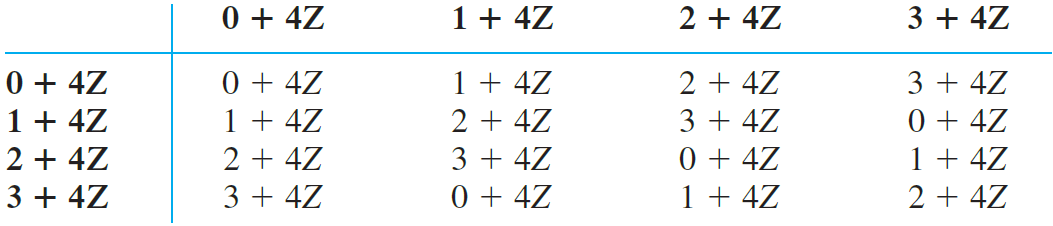
\includegraphics[width=0.9\linewidth]{figures/example 9.10.png}
            \caption{The Cayley table of $\mathbb{Z}/4\mathbb{Z}$.}
            \label{example9.10}
        \end{figure}
     \end{example}
     
     \begin{example}
        Let $G=\mathbb{Z}_{18}$ and $H=\langle 6 \rangle = \{6,12,0\}$. Then since
        \begin{align*}
            0 + H &= H = 6 + H = 12 + H, \\
            1 + H &= \{1, 7, 13 \} = 7 + H = 13 + H, \\
            2 + H &= \{ 2, 8, 14 \} = 8+H = 14+H, \\
            3 + H &= \{ 3, 9, 15 \} = 9+H = 15+H, \\
            4 + H &= \{ 4, 10, 16 \} = 10+H = 16+H, \\
            5 + H &= \{ 5, 11, 15 \} = 11+H = 17+H,
        \end{align*}
        it follows that $G/H = \{0+H,1+H,2+H,3+H,4+H,5+H\}$. Consider $(5+H)+(4+H)$,
        \begin{align*}
            (5+H)+(4+H) &= 5+4+H \\
            &= 9+H \\
            &= 3+6+H \\
            &= 3+\{6,12,0\} \\
            &= 3+H.
        \end{align*}
     \end{example}
     
     \begin{example}
        Let $\mathfrak{K} = \{R_0,R_{180}\}$, and consider the factor group of $D_4$
        \begin{equation*}
            D_4/\mathfrak{K} = \{\mathfrak{K},R_{90}\mathfrak{K},H\mathfrak{K},D\mathfrak{K}\}.
        \end{equation*}
        Figure \ref{table9.1} shows the Cayley table for $D_4\mathfrak{K}$.
        
        $D_4/\mathfrak{K}$ provides a good opportunity to demonstrate how a factor group of $G$ is related to $G$ itself. Arrange the heading of the Cayley table for $D_4$ in such a way that elements from the same coset of $\mathfrak{K}$ are in adjacent columns as shown in Figure \ref{table9.2}. Then, the multiplication table for $D_4$ can be blocked off into boxes that are cosets of $\mathfrak{K}$, and the substitution that replaces a box containing the element $x$ with the coset $x\mathfrak{K}$ yields the Cayley table for $D_4/\mathfrak{K}$.
        
        For example, when one passes from $D_4$ to $D_4/\mathfrak{K}$, the box shown in Figure \ref{box1} in Figure \ref{table9.2} becomes the element $H\mathfrak{K}$ in Figure \ref{table9.1}. Similarly, the box shown in Figure \ref{box2} becomes the element $D\mathfrak{K}$, and so on.
        
        In this way, one can see that the formation of a factor group $G/H$ causes a systematic collapse of the elements of $G$. In particular, all the elements in the coset of $H$ containing $a$ collapse to the single group element $aH$ in $G/H$.
        
        \begin{figure}[!htbp]
            \centering
            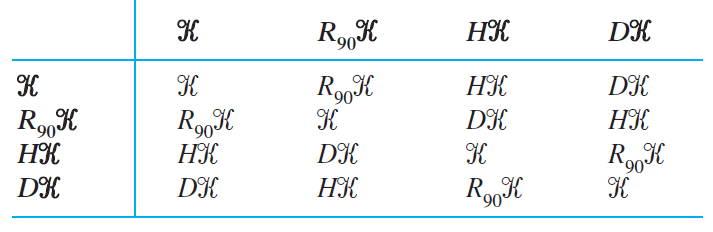
\includegraphics[width=0.8\linewidth]{figures/table9.1.png}
            \caption{}
            \label{table9.1}
        \end{figure}
        
        \begin{figure}[!htbp]
            \centering
            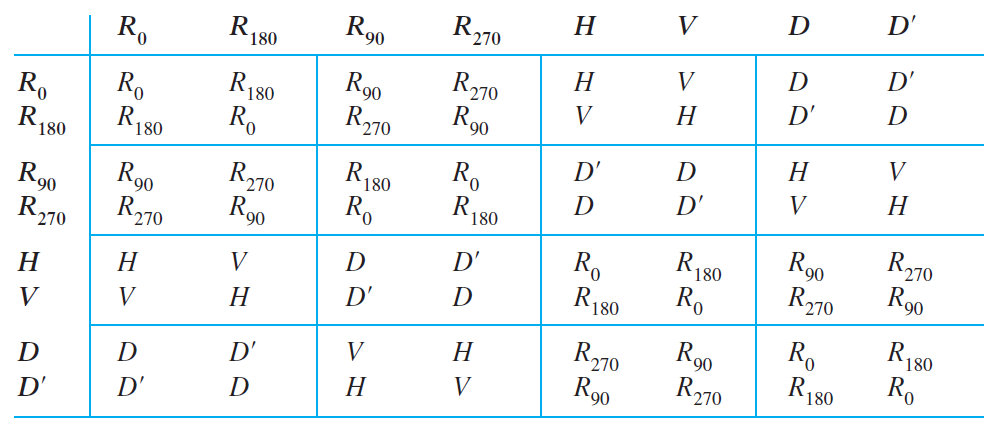
\includegraphics[width=\linewidth]{figures/table9.2.png}
            \caption{}
            \label{table9.2}
        \end{figure}
        
        \begin{figure}[!htbp]
            \centering
            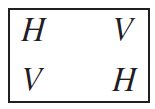
\includegraphics[width=0.2\linewidth]{figures/box1.png}
            \caption{}
            \label{box1}
        \end{figure}
        
        \begin{figure}[!htbp]
            \centering
            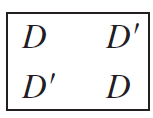
\includegraphics[width=0.2\linewidth]{figures/box2.png}
            \caption{}
            \label{box2}
        \end{figure}
     \end{example}
     
        
     \begin{example}
        Let 
        \begin{equation*}
            G = U(32) = \{1,3,5,7,9,11,13,15,17,19,21,23,25,27,29,31\}
        \end{equation*}
        and $H = U_{16}(32) = \{1,17\}$. Since
        \begin{align*}
            1H1^{-1} &= 1H1 = H \subseteq H \\
            3H3^{-1} &= 3H11 = \{3,51\}11 = \{3,19\}11 = \{33,209\} = \{1,17\} = H \subseteq H, \\
            5H5^{-1} &= 5H13 = \{5,85\}13 = \{5,21\}13 = \{65,273\} = \{1,17\} = H \subseteq H, \\
            & \vdots \\
            31H31^{-1} &= 31H31 = \{31,527\}31 = \{31,15\}31 = \{961,465\} = \{1,17\} = H \subseteq H,
        \end{align*}
        hence by Theorem 9.1, $H \lhd G$. Since
        \begin{align*}
            1H &= \{1,17\}, \\
            3H &= \{3,51\} = \{3,19\}, \\
            5H &= \{5,85\} = \{5,21\}, \\
            7H &= \{7,119\} = \{7,23\}, \\
            9H &= \{9,25\}, \\
            11H &= \{11,27\}, \\
            13H &= \{13,29\}, \\
            15H &= \{15,31\}, \\
            17H &= \{17,1\} = 1H, \\
            & \vdots \\
            31H &= \{31,15\} = 15H,
        \end{align*}
        it follows that $G/H = \{1H,3H,5H,7H,9H,11H,13H,15H\}$ with the operation $(aH)(bH) = abH$ is a factor group and $|G/H| = |G|/|H| = 16/2 = 8$. Since 
        \begin{equation*}
            (1H)(kH) = kH = (kH)(1H), k \in \{1,3,5,\dots,15\},
        \end{equation*}
        $(1H) \in G/H$ is the identity. Since
        \begin{align*}
            (3H)(5H) &= 15H = (5H)(3H), \\
            (3H)(7H) &= 21H = \{21,357\} = \{21,5\} = 5H = (7H)(3H), \\
            (7H)(9H) &= 63H = \{63,1071\} = \{31,15\} = 15H = (9H)(7H), \\
            & \vdots \\
            (aH)(bH) &= (bH)(aH) \in G/H, a,b \in \{1,3,5,\dots,15\},
        \end{align*}
        it follows that $G/H$ is Abelian. 
        \\ \\
        There are three possible Abelian groups of order 8, namely,
        \begin{align*}
            \mathbb{Z}_8 &= \{0,1,\dots,7\}, \\
            \mathbb{Z}_4 \oplus \mathbb{Z}_2 &= \{(0,0),(0,1),(1,0),(1,1),(2,0),(2,1),(3,0),(3,1)\}, \\
            \mathbb{Z}_2 \oplus \mathbb{Z}_2 \oplus \mathbb{Z}_2 &= \{(0,0,0),(0,0,1),(0,1,0),(0,1,1), \\
            & \quad \quad (1,0,0),(1,0,1),(1,1,0),(1,1,1)\}.
        \end{align*}
        Since 
        \begin{equation*}
            (3H)^4 = 81H = 1H \implies |3H| = 4,
        \end{equation*}
        it follows that $G/H$ is not isomorphic to $\mathbb{Z}_2 \oplus \mathbb{Z}_2 \oplus \mathbb{Z}_2$ since 
        \begin{equation*}
            \neg \exists a \in \mathbb{Z}_2 \oplus \mathbb{Z}_2 \oplus \mathbb{Z}_2: |a| = 4.
        \end{equation*}
        Since $\mathbb{Z}_8=\langle 3 \rangle$ and $|\mathbb{Z}_8|=8$, by Theorem 4.4, 
        \begin{equation*}
             2 \mid 8, 2 \in \mathbb{N} \implies \text{number of } a \in \mathbb{Z}_8: |a|=2 \text{ is } \phi(2) = 1.
        \end{equation*}
        Since $|7H|=2$ and $|9H|=2$, there is more than an element of order 2 and $G/H$ is not isomorphic to $\mathbb{Z}_8$. Hence $U(32)/U_{16}(32) \approx \mathbb{Z}_4 \oplus \mathbb{Z}_2$, which is also isomorphic to $U(16)$.
     \end{example}
     
     \begin{example}
        Let $G = \mathbb{Z}_8 \oplus \mathbb{Z}_4 = \{(0,0),(0,1),(0,2),(0,3),\dots,(7,2),(7,3)\}$ and $H = \langle (2,2) \rangle$. Since
        \begin{align*}
            1(2,2) &= (2,2), & 0(2,2) &= (0,0) \\
            2(2,2) &= (4,4) = (4,0), & -1(2,2) &= (-2,-2) = (6,2), \\
            3(2,2) &= (6,6) = (6,2), & -2(2,2) &= (-4,-4) = (4,0), \\
            4(2,2) &= (8,8) = (0,0), & -3(2,2) &= (-6,-6) = (2,2) \\
            5(2,2) &= (10,10) = (2,2), & -4(2,2) &= (-8,-8) = (0,0), \\
            & \vdots & \vdots
        \end{align*}
        it follows that $H = \langle (2,2) \rangle = \{(2,2),(4,0),(6,2),(0,0)\}$. Since
        \begin{align*}
            (0,0)H(0,0)^{-1} &= (0,0)H(0,0) = H \subseteq H, \\
            (0,1)H(0,1)^{-1} &= (0,1)H(0,3) \\
            &= \{(2,3),(4,1),(6,3),(0,1)\}(0,3) \\
            &=\{(2,6),(4,4),(6,6),(0,4)\} \\
            &=\{(2,2),(4,0),(6,2),(0,0\} = H \subseteq H, \\
            & \vdots \\
            (7,3)H(7,3)^{-1} &= (7,3)H(1,1) \\
            &= \{(9,5),(11,3),(13,5),(7,3)\}(1,1) \\
            &= \{(1,1),(3,3),(5,1),(7,3)\}(1,1) \\
            &= \{(2,2),(4,4),(6,2),(8,4)\} \\
            &= \{(2,2),(4,0),(6,2),(0,0)\} = H \subseteq H,
        \end{align*}
        by Theorem 9.1, $H \lhd G$. Hence $G/H$ with the operation $(aH)(bH) = abH$ is a factor group. Since
        \begin{align*}
            (0,0)H &= \{(2,2),(4,0),(6,2),(0,0)\}, \\
            (0,1)H &= \{(2,3),(4,1),(6,3),(0,1)\}, \\
            (0,2)H &= \{(2,4),(4,2),(6,4),(0,2)\} = \{(2,0),(4,2),(6,0),(0,2)\}, \\
            (0,3)H &= \{(2,5),(4,3),(6,5),(0,3)\} = \{(2,1),(4,3),(6,1),(0,3)\}, \\
            (1,0)H &= \{(3,2),(5,0),(7,2),(1,0)\}, \\
            (1,1)H &= \{(3,3),(5,1),(7,3),(1,1)\} \\
            (1,2)H &= \{(3,4),(5,2),(7,4),(2,2)\} = \{(3,0),(5,2),(7,0),(2,2)\}, \\
            (1,3)H &= \{(3,5),(5,3),(7,5),(2,3)\} = \{(3,5),(5,3),(7,1),(2,3)\} \\
            (2,0)H &= \{(4,2),(6,0),(8,2),(2,0)\} = \{(4,2),(6,0),(0,2),(2,0)\} = (0,2)H, \\
            (2,1)H &= \{(4,3),(6,1),(8,3),(2,1)\} = \{(4,3),(6,1),(0,3),(2,1)\} = (0,3)H, \\
            & \vdots
        \end{align*}
        it follows that
        \begin{equation*}
            G/H = \{(0,0)H,(0,1)H,(0,2)H,(0,3)H,(1,0)H,(1,1)H,(1,2)H,(1,3)H\}
        \end{equation*}
        and $|G/H| = 8$. Hence $G/H$ is isomorphic to one of $\mathbb{Z}_8, \mathbb{Z}_4 \oplus \mathbb{Z}_2$ and $\mathbb{Z}_2 \oplus \mathbb{Z}_2 \oplus \mathbb{Z}_2$. Since for any $(a,b)H$,
        \begin{equation*}
            ((a,b)H)^4 = ((a,b)^4H) = ((4a,4b)H) = \bigg\{ \begin{matrix}
               (4,0)H & , a \textit{ is odd} \\
               (0,0)H & , a \textit{ is even}
            \end{matrix},
        \end{equation*}
        and $(0,0),(4,0) \in H$, it follows that 
        \begin{equation*}
            ((a,b)H)^4 = ((a,b)^4H) = ((4a,4b)H) = H.
        \end{equation*}
        Hence $\forall (a,b)H \in G/H, |(a,b)H| \leq 4$. Since
        \begin{equation*}
            ((1,0)H)^2 = ((1,0)^2H) = (2,0)H \neq H,
        \end{equation*}
        it follows that $|(1,0)H|=4$. Hence $G/H$ is not isomorphic to $\mathbb{Z}_8$ and $\mathbb{Z}_2 \oplus \mathbb{Z}_2 \oplus \mathbb{Z}_2$.
     \end{example}
     
     \subsection{Applications of Factor Groups}
     \fbox{\parbox{\linewidth}{
     \begin{theorem}
        Let $G$ be a group and let $Z(G)$ be the center of $G$. Then
        \begin{equation*}
            G/Z(G) \text{ is cyclic} \implies G \text{ is Abelian.}
        \end{equation*}
     \end{theorem}
     }}
     
     \begin{proof}
        Let $G$ be a group and let $Z(G)$ be the center of $G$. Assume that $G/Z(G)$ is cyclic. Since
        \begin{equation*}
            Z(G) = \{a \in G: \forall x \in G, ax=xa\},
        \end{equation*}
        the factor group
        \begin{equation*}
            G/Z(G) = \{gZ(G): g \in G\}.
        \end{equation*}
        Since $G/Z(G)$ is cyclic,
        \begin{equation*}
            \exists gZ(G) \in G/Z(G): G/Z(G) = \langle gZ(G) \rangle.
        \end{equation*}
        Let $kZ(G) \in G/Z(G)$ arbitrary, then 
        \begin{equation*}
            \exists i \in \mathbb{Z}: (gZ(G))^i = kZ(G).
        \end{equation*}
        But
        \begin{equation*}
            (gZ(G))^i = g^iZ(G) = kZ(G).
        \end{equation*}
        Since
        \begin{equation*}
            Z(G) \leq G \implies e \in Z(G),
        \end{equation*}
        it follows that
        \begin{equation*}
            k = ke = g^ia, a \in Z(G).
        \end{equation*}
        Let
        \begin{equation*}
            C(g) = \{x \in G: xg=gx\}
        \end{equation*}
        be the center of $g$. Then since
        \begin{align*}
            g^i \in G, g^ig=gg^i \implies g^i \in C(g), \\
            a \in Z(G) \subseteq G, ag=ga \implies a \in C(g),
        \end{align*}
        it follows that $k = g^ia \in C(g)$. Since $k$ is arbitrary,
        \begin{equation*}
            \forall k \in G, kg = gk.
        \end{equation*}
        Hence $g \in Z(G)$ and by Lemma 7.1, 
        \begin{equation*}
            gZ(G) = Z(G) \implies G/Z(G) = \{gZ(G) = Z(G): g \in G\} = \{Z(G)\}.
        \end{equation*}
        Hence $g \in G, \forall x \in G, gx=xg$.
     \end{proof}
     
     \noindent\fbox{\parbox{\linewidth}{
     \begin{theorem}
        Let $G$ be a group. Then $G/Z(G) \approx Inn(G)$.
     \end{theorem}
     }}
     
     \begin{proof}
        Let $G$ be a group. Let
        \begin{equation*}
            G/Z(G) = \{gZ(G):g \in G\}
        \end{equation*}
        and
        \begin{equation*}
            Inn(G) = \{\phi_g(x) = gxg^{-1}: \forall x \in G, g \in G\}. 
        \end{equation*}
        Let $T\big(gZ(G)\big) = \phi_g(x)$. First, let $gZ(G),hZ(G) \in Z(G)$ be arbitrary. Assume that $gZ(G)=hZ(G)$. By Lemma 7.1 (vi),
        \begin{equation*}
            gZ(G) = hZ(G) \iff h^{-1}g \in Z(G).
        \end{equation*}
        It follows that $\forall x \in G, h^{-1}gx = xh^{-1}g$. So
        \begin{align*}
            h^{-1}gx &= xh^{-1}g, \\
            gxg^{-1} &= hxh^{-1}, \\
            \phi_g(x) &= \phi_h(x).
        \end{align*}
        Hence $T: gZ(G) \to \phi_g(x)$ is a function. Second, let assume that $T(gZ(G)) = T(hZ(G))$. Then
        \begin{align*}
            T(gZ(G)) &= T(hZ(G)), \\
            \phi_g(x) &= \phi_(x), \\
            gxg^{-1} &= hxh^{-1}, \\
            h^{-1}gx &= xh^{-1}g, \\
        \end{align*}
        it follows that $h^{-1}g \in Z(G)$. By Lemma 7.1 (vi),
        \begin{equation*}
            gZ(G) = hZ(G) \iff h^{-1}g \in Z(G).
        \end{equation*}
        Hence $T$ is one-to-one. Next, let $\phi_g(x) \in Inn(G)$ be arbitrary. Since $T$ is one-to-one, there exists an inverse function $T^{-1}$ s.t.
        \begin{align*}
            T(gZ(G)) &= \phi_g(x), \\
            gZ(G) &= T^{-1}(\phi_g(x)),
        \end{align*}
        it follows that
        \begin{align*}
            \exists gZ(G) \in G/Z(G): T(gZ(G)) = T(T^{-1}(\phi_g(x))) = \phi_g(x).
        \end{align*}
        Hence $T$ is onto. Finally,
        \begin{align*}
            T(gZ(G)hZ(G)) &= T(ghZ(G)) \\
            &= \phi_{gh}(x) \\
            &= ghx(gh)^{-1} \\
            &= ghxh^{-1}g \\
        \end{align*}
        and
        \begin{align*}
            T(gZ(G))T(hZ(G)) &= \phi_g\phi_h(x) \\
            &= \phi_g(hxh^{-1}) \\
            &= ghxh^{-1}g.
        \end{align*}
        Hence $T$ conserves the operation. It follows that $G/Z(G) \approx Inn(G)$.
        \end{proof}
        
        \begin{example}
        \end{example}
        
        \noindent\fbox{\parbox{\linewidth}{
        \begin{theorem}[Cauchy's Theorem for Abelian Groups]
           Let $G$ be a finite Abelian group and let $p$ be a prime, $p \mid |G|$. Then
           \begin{equation*}
               \exists g \in G: |g| = p.
           \end{equation*}
        \end{theorem}
        }}
        
        \begin{proof}
           Let $G$ be a finite Abelian group and let $p$ be a prime, $p \mid |G|$. If $|G|=2$, then let $p = 2$ and $\exists g \in G: |g|=2$. Hence Theorem 9.5 is true.
           \\ \\
           If $|G| \neq 2$. By the Second Principle of Mathematical Induction, assume that Theorem 9.5 is true for all Abelian groups with orders less than $|G|$. Let $x \in G, |x| = m = qn$, $q$ is prime, then $|x^n| = q$. Hence
           \begin{equation*}
               \exists x^n \in G: |x^n| = q.
           \end{equation*}
           If $q=p$, then Theorem 9.5 is true. If $q \neq p$, since $G$ is Abelian,
           \begin{equation*}
               \langle x \rangle \leq G \implies \langle x \rangle \lhd G.
           \end{equation*}
           Hence
           \begin{equation*}
               \overline{G} = G/\langle x \rangle = \{g\langle x \rangle: g \in G\}
           \end{equation*}
           with the operation $(g\langle x \rangle)(h\langle x \rangle) = gh\langle x \rangle$ is a factor group. Since $G$ is Abelian, $g,h \in G, gh=hg$. It follows that
           \begin{align*}
               g\langle x \rangle, h\langle x \rangle \in \overline{G}, (g\langle x \rangle)(h\langle x \rangle) &= gh\langle x \rangle \\
               &= hg \langle x \rangle \\
               &= (h\langle x \rangle)(g\langle x \rangle).
           \end{align*}
           Hence $\overline{G}$ is Abelian. Since
           \begin{equation*}
               |\overline{G}| = |G/\langle x \rangle| = |G|/|\langle x \rangle| = |G|/q,
           \end{equation*}
           it follows that $|\overline{G}| < |G|$. Hence Theorem 9.5 is true for $|\overline{G}|$. So $p \mid |\overline{G}|$ and
           \begin{equation*}
               \exists y\langle x \rangle \in \overline{G}: |y\langle x \rangle| = p.
           \end{equation*}
           Since $\langle x \rangle$ is the identity element of $|\overline{G}|$, it follows that $(y\langle x \rangle)^p = y^p\langle x \rangle = \langle x \rangle$. Hence $y^p \in \langle x \rangle$. If $y^p = e$, then Theorem 9.5 is true. If $y^p \neq e$, then $|y^p| = q$ and $|y^q| = p$.
        \end{proof}
        
        \subsection{Internal Direct Products}
        \fbox{\parbox{\linewidth}{
        \begin{definition}
            Let $H,K \lhd G$. If
            \begin{equation*}
                \quad G=HK=\{hk:h \in H, k \in K\}, \quad \text{and} \quad H \cap K = \{e\},
            \end{equation*}
            then $G=H\times K$ is the \textit{internal direct product} of $H,K$.
        \end{definition}
        }}
        \\ \\
        Figure \ref{internal_diret_product}
        and \ref{external_direct_product} show the internal direct product and external direct product.
        \begin{figure}[!htbp]
            \centering
            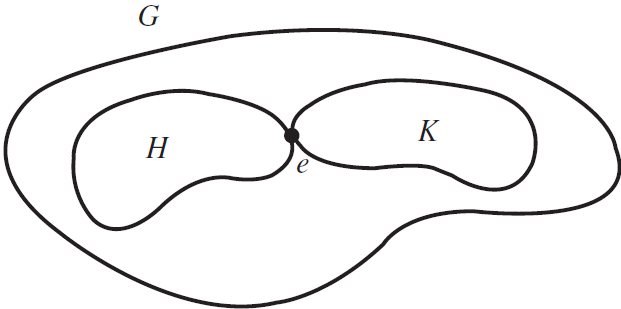
\includegraphics[width=0.6\linewidth]{figures/internal_direct_products.png}
            \caption{For the internal direct product, $H,K$ must be subgroups of the same group.}
            \label{internal_diret_product}
        \end{figure}
        
        \begin{figure}[!htbp]
            \centering
            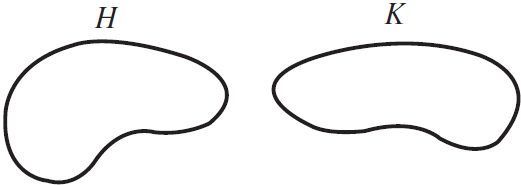
\includegraphics[width=0.6\linewidth]{figures/external_direct_products.png}
            \caption{For the external direct product, $H,K$ can be any groups.}
            \label{external_direct_product}
        \end{figure}
        
        \begin{example}
        If $s,t$ are relatively prime positive integers then $U(st)=U_s(st) \times U_t(st)$.
        \end{example}
        
        \begin{example}
            In $D_6$ let $F \in D_6$ be some reflection and let $R_k \in D_6$ be a rotation of $k$ degrees. Then,
            \begin{equation*}
                D_6 = \{R_0, R_{120}, R_{240}, F, R_{120}F, R_{240}F\} \times \{R_0, R_{180}\}.
            \end{equation*}
        \end{example}
        
        \noindent\fbox{\parbox{\linewidth}{
        \begin{definition}
            Let $H_1,H_2,\dots,H_n \lhd G$. Then $G$ is the \textit{internal direct product} of $H_1,H_2,\dots,H_n$, denoted $G=H_1 \times H_2 \times \dots \times H_n$, if
            \begin{enumerate}
                \item $G = H_1 H_2 \cdots H_n = \{h_1h_2 \dots h_n: h_i \in H_i\}$,
                \item $(H_1H_2 \cdots H_i) \cap H_{i+1} = \{e\}, i=1,2,\dots,n-1$.
            \end{enumerate}
        \end{definition}
        }}
        \\ \\
        \fbox{\parbox{\linewidth}{
        \begin{theorem}
           Let $G$ be a group. Then
           \begin{equation*}
               G = H_1 \times H_2 \times \dots \times H_n \implies G \approx H_1 \oplus H_2 \oplus \dots \oplus H_n.
           \end{equation*}
        \end{theorem}
        }}
        \begin{proof}
           Let $G$ be a group and assume that $G = H_1 \times H_2 \times \dots \times H_n$. So $H_1,H_2,\dots,H_n \lhd G$,
           \begin{equation*}
                G = H_1 H_2 \cdots H_n = \{h_1h_2 \dots h_n: h_i \in H_i\},
            \end{equation*}
            and
            \begin{equation*}
                (H_1H_2 \cdots H_i) \cap H_{i+1} = \{e\}, i=1,2,\dots,n-1.
            \end{equation*}
           Let $h_i \in H_i, h_j \in H_j, i \neq j$, then by Theorem 9.1,
           \begin{equation*}
               H \lhd G \iff \forall x \in G, xHx^{-1} \subseteq H.
           \end{equation*}
           So
           \begin{equation*}
               h_jh_ih_j^{-1} \in h_jH_ih_j^{-1} \subseteq H_i
           \end{equation*}
           and
           \begin{equation*}
               h_ih_jh_i^{-1} \in h_iH_jh_i^{-1} \subseteq H_j.
           \end{equation*}
           It follows that
           \begin{equation*}
               (h_ih_jh_i^{-1})h_j^{-1} \in H_jh_j^{-1} = H_j
           \end{equation*}
           and
           \begin{equation*}
               h_i(h_jh_i^{-1}h_j^{-1}) \in h_iH_i = H_i.
           \end{equation*}
           Hence,
           \begin{equation*}
               h_ih_jh_i^{-1}h_j^{-1} \in H_i \cap H_j = \{e\} \implies h_ih_jh_i^{-1}h_j^{-1} = e \implies h_ih_j=h_jh_i.
           \end{equation*}
           
           Next, let $g \in G$,
           \begin{equation*}
               g=h_1h_2 \cdots h_n \quad \text{and} \quad g = h_1'h_2' \dots h_n'
           \end{equation*}
           where $h_i,h_i' \in H_i, i=1,\dots,n$. Then, since $h_ih_j=h_jh_i$, it follows that
           \begin{align*}
                g &= g, \\
                h_1h_2 \cdots h_n &= h_1'h_2' \cdots h_n', \\
                h_n'h_n^{-1} &= (h_1')^{-1}h_1(h_2')^{-1}h_2 \cdots (h_{n-1}')^{-1}h_{n-1}.
           \end{align*}
           Therefore
           \begin{equation*}
               h_n'h_n^{-1} \in (H_1H_2 \cdots H_{n-1}) \cap H_n = \{e\},
           \end{equation*}
           it follows that
           \begin{equation*}
               h_n'h_n^{-1} = e \implies h_n' = h_n.
           \end{equation*}
           So
           \begin{align*}
               h_1h_2 \cdots h_n &= h_1'h_2' \cdots h_n', \\
               h_1h_2 \cdots h_{n-1} &= h_1'h_2' \cdots h_n'h_n^{-1}, \\
               h_1h_2 \cdots h_{n-1} &= h_1'h_2' \cdots h_{n-1}'e, \\
               h_1h_2 \cdots h_{n-1} &= h_1'h_2' \cdots h_{n-1}'.
           \end{align*}
           Repeating the steps,
           \begin{equation*}
               h_{n-1}'h_{n-1}^{-1} = e \implies h_{n-1}'=h_{n-1}.
           \end{equation*}
           Continuing the process, eventually
           \begin{equation*}
               h_i' = h_i, i = 1,\dots,n.
           \end{equation*}
           
           Define $\phi: G \to H_1 \oplus H_2 \oplus \cdots \oplus H_n$ by $\phi(h_1h_2 \cdots h_n) = (h_1,h_2,\dots,h_n)$. First, assume that $h_1h_2 \cdots h_n, h_1'h_2' \cdots h_n' \in G, h_1h_2 \cdots h_n = h_1'h_2' \cdots h_n'$. Then
           \begin{align*}
               \phi(h_1h_2 \cdots h_n) &= (h_1,h_2,\dots,h_n) \\
               &= (h_1',h_2',\dots,h_n') \\
               &= \phi(h_1'h_2' \cdots h_n').
           \end{align*}
           So $\phi$ is a well-defined function. Second, assume that $\phi(h_1h_2 \cdots h_n) = \phi(h_1'h_2' \cdots h_n')$. Then since $h_i' = h_i, i = 1,\dots,n$, it follows that
           \begin{align*}
               h_1h_2 \cdots h_n = h_1'h_2' \cdots h_n'.
           \end{align*}
           Hence $\phi$ is one-to-one. Third, let $(h_1,h_2,\dots,h_n) \in H_1 \oplus \cdots \oplus H_n$ be arbitrary. Since
           \begin{align*}
               \phi(h_1 \cdots h_n) &= (h_1,\dots,h_n), \\
               h_1 \cdots h_n &= \phi^{-1}((h_1, \dots, h_n)).
           \end{align*}
           Let $h_1 \cdots h_n = \phi^{-1}((h_1, \dots, h_n))$, it follows that
           \begin{equation*}
               \phi(h_1 \cdots h_n) = \phi(\phi^{-1}((h_1, \dots, h_n))) = (h_1, \dots, h_n).
           \end{equation*}
           Hence $\phi$ is onto. Finally,
           \begin{align*}
               \phi((h_1 \cdots h_n)(h_1' \cdots h_n')) &= \phi(h_1h_1' \cdots h_nh_n') \\
               &= (h_1h_1',\dots,h_nh_n') \\
               &= (h_1,\dots,h_n)(h_1',\dots,h_n') \\
               &= \phi(h_1 \cdots h_n)\phi(h_1' \cdots h_n').
           \end{align*}
           Hence $\phi$ preserves the operation. Therefore, $G \approx H_1 \oplus \cdots \oplus H_n$.
        \end{proof}
        
        \noindent\fbox{\parbox{\linewidth}{
        \begin{theorem}
           Let $G$ be a group and $p$ a prime. Then
           \begin{equation*}
               |G|=p^2 \implies G \approx \mathbb{Z}_{p^2} \quad \text{or} \quad G \approx \mathbb{Z}_p \oplus \mathbb{Z}_p. 
           \end{equation*}
        \end{theorem}
        }}
        
        \begin{proof}
        \end{proof}
        
        \noindent\fbox{\parbox{\linewidth}{
        \begin{corollary}
                Let $G$ be a group and $p$ a prime. Then
                \begin{equation*}
                    |G| = p^2 \implies \forall a,b \in G, ab = ba.
                \end{equation*}
        \end{corollary}
        }}
        
\section{Group Homomorphisms}
    \fbox{\parbox{\linewidth}{
    \begin{definition}
        A \textit{homomorphism} $\phi:G\to\overline{G}$ is a mapping that preserves the group operation; that is, $\forall a,b \in G, \phi(ab) = \phi(a)\phi(b)$.
    \end{definition}
    }}
    \\ \\
    \noindent\fbox{\parbox{\linewidth}{
    \begin{definition}
        The \textit{kernel} of a homomorphism $\phi$ from a group $G$ to a group with identity $e$ is the set $\{x \in G: \phi(x) = e\}$, denoted by $\Ker \phi$. Moreover, $\Ker\phi \lhd G$.
        \end{definition}
    }}
    
    \begin{example}
        Any isomorphism is a homomorphism that is also one-to-one and onto. The kernel of an isomorphism is the trivial subgroup.
    \end{example}
    
    \begin{example}
        Let $\mathbb{R}^* = \mathbb{R} \setminus \{0\}$ under multiplication.. Then the determinant mapping $A \to \det A$ is a homomorphism from $GL(2,\mathbb{R})$ to $\mathbb{R}^*$. The kernel of the determinant mapping is $SL(2,\mathbb{R})$.
    \end{example}
    
    \begin{example}
        The mapping $\phi:\mathbb{R}^* \to \mathbb{R}^*, \phi(x)=|x|$ is a homomorphism with $\Ker\phi=\{-1,1\}$.
    \end{example}
    
    \begin{example}
        Let $\mathbb{R}[x]$ be the group of all polynomials with real coefficients under addition. For $f \in \mathbb{R}[x]$, let $f'$ be the derivative of $f$. Then $\phi(f) = f'$ is a homomorphism $\phi:\mathbb{R}[x] \to \mathbb{R}[x]$. $\Ker\phi$ is the set of all constant polynomials.
    \end{example}
    
    \begin{example}
        The mapping $\mathbb{Z} \to \mathbb{Z}_n, \phi(m) = m \mod{n}$, is a homomorphism and $\Ker\phi=\langle n \rangle$.
    \end{example}
    
    \begin{example}
        The mapping $\phi: \mathbb{R}^* \to \mathbb{R}^*, \phi(x)=x^2$, under multiplication is a homomorphism, since $a,b \in \mathbb{R}^*, \phi(ab) = (ab)^2 = a^2b^2 = \phi(a)\phi(b)$. $\Ker\phi = \{-1,1\}$.
    \end{example}
    
    \begin{example}
        The mapping $\phi:\mathbb{R} \to \mathbb{R}, \phi(x)=x^2$ under addtion is not a homomorphism, since $a,b \in \mathbb{R}, \phi(a+b) = (a+b)^2 = a^2+2ab+b^2 \neq a^2+b^2 = \phi(a) = \phi(b)$.
    \end{example}
    
    \subsection{Properties of Homomorphisms}
    \fbox{\parbox{\linewidth}{
    \begin{theorem}
       Let $\phi:G \to \overline{G}$ be a homomorphism, let $g \in G$. Then
       \begin{enumerate}
           \item $e \in G, \overline{e} \in \overline{G}, \phi(e)=\overline{e}.$
           \item $\forall n \in \mathbb{Z}, \phi(g^n) = (\phi(g))^n.$
           \item $|g| = n \implies |\phi(g)| \mid |g|$.
           \item $\Ker \phi \leq G$.
           \item $\phi(a) = \phi(b) \iff a\Ker\phi = b\Ker\phi$.
           \item $\phi(g) = \overline{g} \implies \phi^{-1}(\overline{g}) = \{x \in G : \phi(x)  =\overline{g}\} = g\Ker\phi$. (!)
       \end{enumerate}
    \end{theorem}
    }}
    
    \begin{proof}
       Let $\phi:G \to \overline{G}$ be a homomorphism, $g \in G$.
       \begin{enumerate}
           \item Let $e \in G, \overline{e} \in \overline{G}$. Since $phi$ is OP, $\phi(g) \in \overline{G}$,
           \begin{equation*}
               \phi(g)\phi(e) = \phi(ge) = \phi(g) = \phi(eg) = \phi(e)\phi(g).
           \end{equation*}
           Hence $\phi(e) = \overline{e}$.
           \item Let $n \in \mathbb{Z}$ be arbitrary, since $\phi$ is OP,
           \begin{align*}
               \phi(g^n) &= \underbrace{\phi(g)\cdots\phi(g)}_n = (\phi(g))^n.
           \end{align*}
           \item Let $|g|=n$, then
           \begin{align*}
               (\phi(g))^n &= \phi(g^n) = \phi(e) = \overline{e}.
           \end{align*}
           By Theorem 4.1(ii),
           \begin{equation*}
               (\phi(g))^n = \overline{e} = (\phi(g))^0 \iff |\phi(g)| \mid (n-0) = n.
           \end{equation*}
           \item Let $\Ker\phi=\{g\in G: \phi(g)=\overline{e}, g,g^{-1} \in \Ker\phi$, then
           \begin{equation*}
               \phi(gg^{-1}) = \phi(e) = \overline{e} \implies gg^{-1} \in \Ker\phi.
           \end{equation*}
           Hence by one-step subgroup test, $\Ker\phi \leq G$.
           \item $(\Rightarrow)$ Let $\phi(a) = \phi(b)$, then
           \begin{align*}
               \overline{e} = \phi(a)(\phi(b))^{-1} = \phi(a)\phi(b^{-1}) = \phi(ab^{-1}),
           \end{align*}
           Hence $ab^{-1}\in \ker\phi$. Since by Theorem 10.1.4, $\Ker\phi \leq G$, by Lemma 7.1.6,
           \begin{equation*}
               ab^{-1} \in \Ker\phi \iff a\Ker\phi = b\Ker\phi.
           \end{equation*} 
           $(\Leftarrow)$ Let $a\Ker\phi = b\Ker\phi$, then by Lemma 7.1.6,
           \begin{equation*}
               ab^{-1} \in \Ker\phi \iff a\Ker\phi = b\Ker\phi.
           \end{equation*}
           Hence,
           \begin{align*}
               \overline{e} = \phi(ab^{-1}) = \phi(a)\phi(b^{-1}) = \phi(a)(\phi(b))^{-1} \implies \phi(a)=\phi(b).
           \end{align*}
           Therefore, $\phi(a) = \phi(b) \iff a\Ker\phi = b\Ker\phi$.
           \item Let $\phi(g)=\overline{g}, \phi^{-1}(\overline{g})=\{x\in G:\phi(x)=\overline{g}\},g\Ker\phi=\{gx:\phi(x)=\overline{e}\}$. Let $x \in \phi^{-1}(\overline{g})$, then
           \begin{equation*}
               \phi(x) = \overline{g} = \phi(g).
           \end{equation*}
           By Theorem 10.1.5,
           \begin{equation*}
               \phi(x) = \phi(g) \iff x\Ker\phi = g\Ker\phi.
           \end{equation*}
           Since $\phi(e)=\overline{e} \implies e \in \Ker\phi$, it follows that
           \begin{equation*}
               x = xe \in x\Ker\phi = g\Ker\phi.
           \end{equation*}
           Hence, $\phi^{-1}(\overline{g}) \subseteq g\ker\phi$.
           
           Let $gx \in g\ker\phi$, then
           \begin{equation*}
               \phi(gx) = \phi(g)\phi(x) = \overline{g}\overline{e} = \overline{g} \implies gx \in \phi^{-1}(\overline{g}).
           \end{equation*}
           Hence $g\ker\phi \subseteq \phi^{-1}(\overline{g})$.
           
           Therefore $\phi^{-1}(\overline{g})=g\ker\phi$.
       \end{enumerate}
    \end{proof}
    
    \noindent\fbox{\parbox{\linewidth}{
    \begin{theorem}
       Let $\phi:G \to \overline{G}$ be a homomorphism, let $H \leq G$. Then
        \begin{enumerate}
            \item $\phi(H) = \{\phi(h):h \in H\} \leq \overline{G}$.
            \item $H$ is cyclic $\implies \phi(H)$ is cyclic. 
            \item $H$ is Abelian $\implies \phi(H)$ is Abelian. 
            \item $H \lhd G \implies \phi(H) \lhd \phi(G)$.
            \item $|\Ker\phi|=n \implies \phi:G \to \phi(G)$ is an $n$-to-1 mapping.
            \item $H$ is finite $\implies |\phi(H)| \mid |H|$.
            \item $\overline{K} \leq \overline{G} \implies \phi^{-1}(\overline{K}) = \{k \in G: \phi(k) \in \overline{K}\} \leq G$.
            \item $\overline{K} \lhd \overline{G} \implies \phi^{-1}(\overline{K}) = \{k \in G: \phi(k) \in \overline{K}\} \lhd G$.
            \item $\phi$ is onto and $\Ker\phi = \{e\} \implies$ $\phi:G \to \overline{G}$ is an isomorphism.
        \end{enumerate}
    \end{theorem}
    }}
    
    \begin{proof}
       Let $\phi:G \to \overline{G}$ be a homomorphism, and $H \leq G$.
       \begin{enumerate}
           \item Let $\phi(H) = \{\phi(h):h\in H\} \subseteq \overline{G}$. Let $\phi(h_1),\phi(h_2) \in \phi(H)$, then since $\phi$ is OP,
           \begin{equation*}
               \phi(h_1)(\phi(h_2))^{-1} = \phi(h_1)\phi(h_2^{-1}) = \phi(h_1h_2^{-1}).
           \end{equation*}
           Hence,
           \begin{equation*}
               h_1h_2^{-1} \in H \implies \phi(h_1)(\phi(h_2))^{-1} = \phi(h_1h_2^{-1}) \in \phi(H).
           \end{equation*}
           By one-step subgroup test, $\phi(H) \leq \overline{G}$.
           \item Let $H = \langle h \rangle, h \in H$, then $x \in H, x=h^n, n \in \mathbb{Z}$. Let $\phi(x) \in \phi(H)$ be arbitrary, then
           \begin{equation*}
               \phi(x) = \phi(h^n) = (\phi(h))^n.
           \end{equation*}
           Hence $\phi(H) = \langle \phi(h) \rangle$.
           \item Let $H$ be Abelian, then $a,b \in H, ab=ba$. Let $\phi(a),\phi(b) \in \phi(H)$, then
           \begin{equation*}
               \phi(a)\phi(b) = \phi(ab) = \phi(ba) = \phi(b)\phi(a).
           \end{equation*}
           Hence $\phi(H)$ is Abelian.
           \item Let $H \lhd G$, then by Theorem 9.1,
           \begin{equation*}
               H \lhd G \iff g \in G, gHg^{-1} \subseteq H.
           \end{equation*}
           Let $\phi(g) \in \phi(G), \phi(h) \in \phi(H)$, then
           \begin{equation*}
               \phi(g)\phi(h)(\phi(g))^{-1} = \phi(g)\phi(h)\phi(g^{-1}) = \phi(ghg^{-1}).
           \end{equation*}
           Since $ghg^{-1} \in gHg^{-1} \subseteq H$, by definition, $\phi(ghg^{-1}) \in \phi(H)$. Hence,
           \begin{equation*}
               \phi(g)\phi(h)(\phi(g))^{-1} = \phi(ghg^{-1}) \in \phi(H) \implies \phi(g)\phi(H)(\phi(g))^{-1} \subseteq \phi(H)
           \end{equation*}
           Therefore by Theorem 9.1,
           \begin{equation*}
               \phi(g)\phi(H)(\phi(g))^{-1} \subseteq \phi(H) \iff \phi(H) \lhd \phi(G).
           \end{equation*}
           \item Let $|\Ker\phi|=n,g\in G, \overline{g}\in\phi(G)$. Then by Theorem 10.1.6,
           \begin{equation*}
               \phi(g) = \overline{g} \implies \phi^{-1}(\overline{g}) = \{x\in G: \phi(x) = \overline{g}\} = g\Ker\phi.
           \end{equation*}
           Hence,
           \begin{equation*}
               |\ker\phi|=n \implies|g\Ker\phi|=n=|\phi^{-1}(\overline{g})|.
           \end{equation*}
           Therefore,
           \begin{equation*}
               \overline{g} \in \phi(g), \exists x_1,\dots,x_n \in G: \phi(x_1)=\dots=\phi(x_n)=\overline{g}.
           \end{equation*}
           \item Let $|H|=n$. Let $\phi_H: H \to \phi(H)$, then $\phi_H$ is a homomorphism. Since
           \begin{equation*}
               H \leq G \implies e \in H \implies \phi(e) \in \phi(H),
           \end{equation*}
           therefore $\Ker\phi_H \neq \emptyset$. Let $|\Ker\phi_H|=t$, by Theoremn 10.2.5, $|\Ker\phi_H|=t \implies \phi_H:H\to\phi(H)$ is $t$-to-1. Hence,
           \begin{equation*}
               |\phi(H)|=|H|/t \implies |\phi(H)|\mid|H|=n.
           \end{equation*}
           \item Let $\overline{K} \leq \overline{G}$ and $\phi^{-1}(\overline{K}) = \{k\in G: \phi(k) \in \overline{K}\} \subseteq G$. Since
           \begin{equation*}
               e \in G, \phi(e) = \overline{e} \in \overline{K} \implies e \in \phi^{-1}(\overline{K}),
           \end{equation*}
           therefore $\phi^{-1}(\overline{K}) \neq \emptyset$. Let $a,b \in \phi^{-1}(\overline{K})$, then $\phi(a),\phi(b) \in \overline{K}$. Since $\phi$ is OP,
           \begin{equation*}
               \phi(ab^{-1}) = \phi(a)\phi(b^{-1}) = \phi(a)(\phi(b))^{-1}.
           \end{equation*}
           Since $\overline{K} \leq \overline{G} \implies \phi(a)(\phi(b))^{-1} \in \overline{K}$, therefore
           \begin{equation*}
               \phi(ab^{-1}) = \phi(a)(\phi(b))^{-1} \in \overline{K} \implies ab^{-1} \in \phi^{-1}(\overline{K}).
           \end{equation*}
           Hence by one-step subgroup test, $\phi^{-1}(\overline{K}) \leq G$.
           \item Let $\overline{K} \lhd \overline{G}$ and $\phi^{-1}(\overline{K})=\{k\in G:\phi(k)\in\overline{K}\}$. Let $a \in \phi^{-1}(\overline{K}), g\in G$. Then since $\phi$ is OP,
           \begin{equation*}
               \phi(gag^{-1}) = \phi(g)\phi(a)\phi(g^{-1}) = \phi(g)\phi(a)(\phi(g))^{-1}.
           \end{equation*}
           Since $\overline{K} \lhd \overline{G}$, therefore $\phi(g) \in \overline{G}, \phi(a) \in \overline{K}$,
           \begin{equation*}
               \phi(g)\overline{K}(\phi(g))^{-1} \subseteq \overline{K} \implies \phi(g)\phi(a)(\phi(g))^{-1} \in \overline{K}.
           \end{equation*}
           Hence,
           \begin{equation*}
               \phi(gag^{-1}) = \phi(g)\phi(a)(\phi(g))^{-1} \in \overline{K} \implies gag^{-1} \in\phi^{-1}(\overline{K}).
           \end{equation*}
           Therefore, $g\phi^{-1}(\overline{K})g^{-1} \subseteq \phi^{-1}(\overline{K})$ and by Theorem 9.1, $\phi^{-1}(\overline{K}) \lhd G$.
           \item Let $\phi$ be onto and $\ker\phi=\{e\}$. By Theorem 10.2.5, $|\Ker\phi| = 1 \implies \phi:G\to\overline{G}$ is 1-to-1. Since $\phi$ is 1-to-1, onto, and OP, therefore $\phi$ is an isomorphism.
       \end{enumerate}
    \end{proof}
    
    \noindent\fbox{\parbox{\linewidth}{
    \begin{corollary}
            Let $\phi:G\to\overline{G}$ be a homomorphism. Then $\Ker\phi \lhd G$. 
    \end{corollary}
    }}
    
    \begin{proof}
       Let $\phi:G\to\overline{G}$ be a homomorphism. By Theorem 10.1.4, $\Ker\phi\leq G$. By Theorem 9.1, let $g\in G, x\in \Ker\phi$ be arbitrary, and $gxg^{-1} \in g\Ker\phi g^{-1}$. Then
       \begin{align*}
           \phi(gxg^{-1}) &= \phi(g)\phi(x)\phi(g^{-1}) \\ &= \phi(g)\phi(x)(\phi(g))^{-1} \\
           &= \phi(g)\overline{e}(\phi(g))^{-1} \\
           &= \phi(g)(\phi(g))^{-1} \\
           &= \overline{e}.
       \end{align*}
       Hence $gxg^{-1} \in\Ker\phi \implies g\Ker\phi g^{-1} \subseteq\Ker\phi$. Therefore $\Ker\phi\lhd G$.
    \end{proof}
    
    \begin{example}
        Let $\phi:\mathbb{C}^*\to\mathbb{C}^*,\phi(x)=x^4$ be a mapping. Since for $x,y \in \mathbb{C}^*$,
        \begin{equation*}
            \phi(xy)=(xy)^4=x^4y^4=\phi(x)\phi(y),
        \end{equation*}
        $\phi$ is a homomorphism. Since
        \begin{equation*}
            \Ker\phi=\{x\in\mathbb{C}^*:\phi(x)=x^4=1\}=\{1,-1,i,-i\},
        \end{equation*}
        so, by Theorem 10.2.5, $|\Ker\phi|=4 \implies \phi$ is a 4-to-1 mapping. To find all $x\in\mathbb{C}^*:\phi(x)=2$, since $\phi(\sqrt[4]{2})=(\sqrt[4]{2})^4=2$, by Theorem 10.1.6,
        \begin{equation*}
            \phi^{-1}(2)=\{x\in\mathbb{C}^*:\phi(x)=2\}=\sqrt[4]{2}\Ker\phi=\{\sqrt[4]{2},-\sqrt[4]{2},\sqrt[4]{2}i,-\sqrt[4]{2}i\}.
        \end{equation*}
        
        Finally, let $H=\langle\cos{30^\circ}+i\sin{30^\circ}\rangle$. By Theorem 10.1.3, Theorem 10.2.6, and DeMoivre's Theorem,
        \begin{equation*}
            (r(\cos{\theta}+i\sin{\theta}))^n = r^n(\cos{n\theta}+i\sin{n\theta}).
        \end{equation*}$|H|=12,\phi(H)=\langle\cos{120^\circ+i\sin{120^\circ}}\rangle$, and $|\phi(H)|=3$.
    \end{example}
    
    \begin{figure}[!htbp]
        \centering
        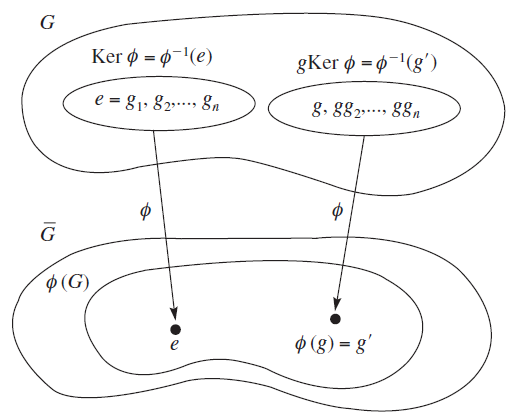
\includegraphics[width=0.6\linewidth]{figures/fig10.1.png}
        \caption{}
        \label{fig10.1}
    \end{figure}
    
    \begin{example}
        Let $\phi:\mathbb{Z}_{12}\to\mathbb{Z}_{12},\phi(x)=3x$ be a mapping. Since for $a,b\in\mathbb{Z}_{12}$,
        \begin{equation*}
            \phi(a+b) = 3(a+b) = 3a+3b = \phi(a)+\phi(b),
        \end{equation*}
        $\phi$ is a homomorphism. Since for $a\in\mathbb{Z}_{12}$,
        \begin{equation*}
            \phi(a)=3a=0 \implies a=0,4,8,
        \end{equation*}
        therefore $\Ker\phi=\{0,4,8\}$. By Theorem 10.2.5, $ |\Ker\phi|=3 \implies$ $\phi$ is a 3-to-1 mapping. Since $\phi(2)=6$, by Theorem 10.1.6,
        \begin{equation*}
            \phi^{-1}(6)=\{a\in\mathbb{Z}_{12}:\phi(a)=6\}=2+\Ker\phi=\{2,6,10\}.
        \end{equation*}
        By Theorem 10.2.2, $\langle2\rangle=\{0,2,4,6,8,10\}$ is cyclic $\implies$ $\phi(\langle2\rangle)=\{0,6\}$ is cyclic. By Theorem 10.1.3,
        \begin{equation*}
            |2|=6 \implies |\phi(2)|=|6|=2||2|=6.
        \end{equation*}
        Let $\overline{K}=\{0,6\} \leq \mathbb{Z}_{12}$, by Theorem 10.2.7,
        \begin{equation*}
            \phi^{-1}(\overline{K}) = \{a\in\mathbb{Z}_{12}:\phi(a)\in\overline{K}\} \leq \mathbb{Z}_{12}.
        \end{equation*}
    \end{example}
    
    \begin{example}
        Both $\mathbb{Z}_{12},\mathbb{Z}_{30}$ are cyclic. To determine all homomorphisms $\phi:\mathbb{Z}_{12}\to\mathbb{Z}_{30}$.  Let $1\in\mathbb{Z}_{12},\phi(1)=a$, by Theorem 10.1.2,
        \begin{equation*}
             x\in\mathbb{Z}_{12},\phi(x) = x\phi(1) = xa.
        \end{equation*}
        By Largange's Theorem, 
        \begin{equation*}
            a\in\mathbb{Z}_{30}, |a|=|\langle a \rangle|\mid30,
        \end{equation*}
        and by Theorem 10.1.3, 
        \begin{equation*}
            1\in\mathbb{Z}_{12}, |1|=12 \implies |\phi(1)|=|a|\mid12. 
        \end{equation*}
        Hence $|a|\in\{1,2,3,6\} \implies a=\{0,15,10,20,5,25\}$. Let $\phi_n(1)=n$, then $\{\phi_0,\phi_{15},\phi_{10},\phi_{20},\phi_5,\phi_{25}\}$ are all the homomorphisms from $\mathbb{Z}_{12}\to\mathbb{Z}_{30}$. For example, let $a,b\in\mathbb{Z}_{12}$, then
        \begin{equation*}
             \phi_{15}(a+b)=(a+b)\phi_{15}(1)=(a+b)15 = 15a+15b = \phi_{15}(a)+\phi_{15}(b).
        \end{equation*}
    \end{example}
    
    \begin{example}
        The mapping $\phi:S_n \to \mathbb{Z}_2$ that takes an even permutation to 0 and an odd permutation to 1 is a homomorphism (Figure \ref{fig10.1}).
    \end{example}
    
    \begin{figure}[!htbp]
        \centering
        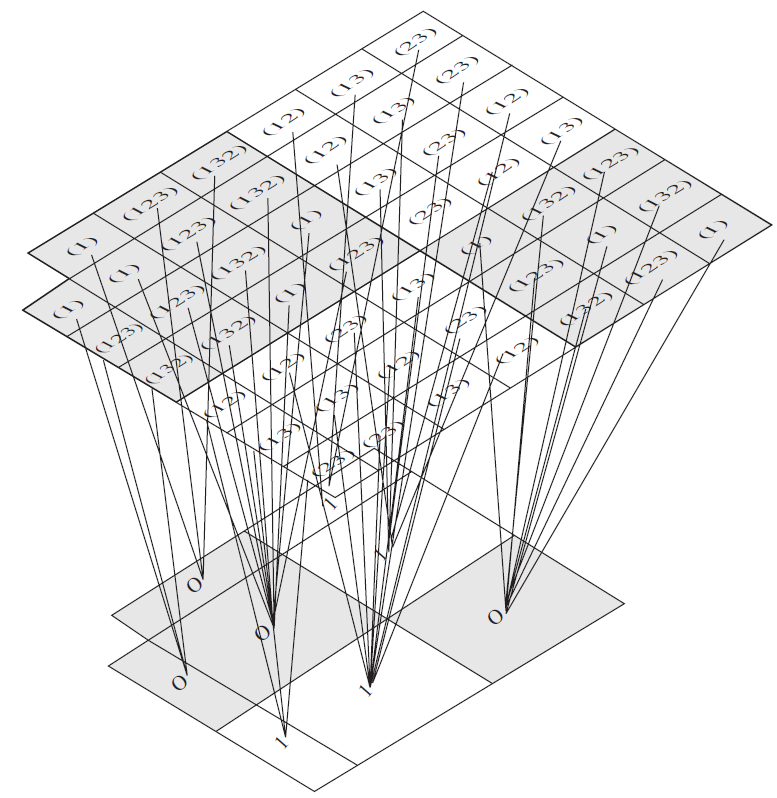
\includegraphics[width=0.8\linewidth]{figures/fig10.2.png}
        \caption{Homomorphism from $S_3$ to $Z_2$.}
        \label{fig10.1}
    \end{figure}
    
    \subsection{The First Isomorphism Theorem}
    \noindent\fbox{\parbox{\linewidth}{
    \begin{theorem}[First Isomorphism Theorem]
       Let $\phi:G \to \overline{G}$ be a homomorphism. Then $\psi:G/\Ker\phi \to \phi(G), \psi(g\Ker\phi) = \phi(g)$ is an isomorphism. In symbols, $G/\Ker\phi \approx \phi(G)$.
    \end{theorem}
    }}
    
    \begin{proof}
       Let $\phi:G \to \overline{G}$ be a homomorphism. Let $\psi:G/\Ker\phi \to \phi(G), \psi(g\Ker\phi) = \phi(g)$ be a mapping. Let $a,b \in G$, by Theorem 10.1.5,
       \begin{equation*}
           \phi(a)=\phi(b) \iff a\Ker\phi = b\Ker\phi.
       \end{equation*}
       Hence $\psi$ is well-defined and 1-to-1. Let $\phi(g) \in \phi(G)$, since
      \begin{equation*}
          g \in G \implies \exists g\Ker\phi\in G/\Ker\phi: \psi(g\Ker\phi)=\phi(g).
      \end{equation*}
      Hence $\psi$ is onto. By Corollary 10.2.1, $\Ker\phi\lhd G$, therefore by Theorem 9.2, $G/\Ker\phi$ under $a\Ker\phi\cdot b\Ker\phi=ab\Ker\phi$ is a factor group. Let $a\Ker\phi,b\Ker\phi\in G/\Ker\phi$, then
      \begin{align*}
          \psi(a\Ker\phi\cdot b\Ker\phi) &= \psi(ab\Ker\phi) \\
          &= \phi(ab) \\
          &= \phi(a)\phi(b) \\
          &= \psi(a\Ker\phi)\psi(b\Ker\phi).
      \end{align*}
      Hence $\psi$ is OP. Therefore $\psi:G/\ker\phi\to\phi(G)$ is an isomorphism and $G/\ker\phi\approx\phi(G)$.
    \end{proof}
    
    \noindent\fbox{\parbox{\linewidth}{
    \begin{corollary}
            Let $G$ be a finite group. Then
            \begin{equation*}
                \phi:G\to\overline{G} \text{ is a homomorphism} \implies |\phi(G)|\mid|G|,|\overline{G}|.
            \end{equation*}
    \end{corollary}
    }}
    
    \begin{proof}
       Let $\phi:G\to\overline{G}$ be a homomorphism. By Theorem 10.1.4, $\Ker\phi\leq G$. By Lagrange's Theorem,
       \begin{equation*}
           |G/\Ker\phi|=|G|/|\Ker\phi| \implies |G/\Ker\phi|\mid|G|.
       \end{equation*}
       By Theorem 10.3,
       \begin{equation*}
           G/\Ker\phi\approx\phi(G) \implies |\phi(G)|=|G/\Ker\phi|\mid|G|.
       \end{equation*}
       By Theorem 10.2.1, 
       \begin{equation*}
           G\leq G \implies \phi(G)\leq\overline{G}.
       \end{equation*}
       Hence by Lagrange's Theorem,
       \begin{equation*}
           \phi(G)\leq\overline{G} \implies |\phi(G)|\mid|\overline{G}|.
       \end{equation*}
       Therefore, $|\phi(G)|\mid|G|,|\overline{G}|$.
    \end{proof}
    
    \begin{example}
        Let $\phi:D_4\to D_4$ be a homomorphism given by Figure \ref{exp10.12}. Then $\Ker\phi=\{R_0,R_{180}\}$. Let $\psi:D_4/\Ker\phi\to\phi(D_4), \psi(x\Ker\phi)=\phi(x),x\in D_4$ be a mapping. So,
        \begin{align*}
            \psi(R_0\Ker\phi)&=\phi(R_0)=R_0=\phi(R_{180})=\psi(R_{180}\Ker\phi), \\ \psi(R_{90}\Ker\phi)&=\phi(R_{90})=H=\phi(R_{270})=\psi(R_{270}\Ker\phi)), \\
            \psi(H\Ker\phi)&=\phi(H)=R_{180}=\phi(V)=\psi(V\Ker\phi), \\
            \psi(D\Ker\phi)&=\phi(D)=V=\phi(D')=\psi(D'\Ker\phi).
        \end{align*}
        By Theorem 10.3, $\psi(D_4/\Ker\phi)\approx\phi(D_4)$.
    \end{example}
    
    \begin{figure}[!htbp]
        \centering
        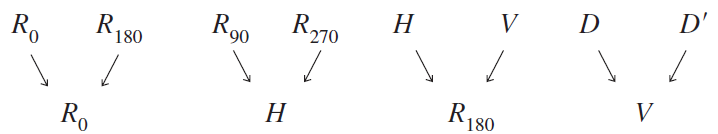
\includegraphics[width=0.7\linewidth]{figures/exp10.12.png}
        \caption{}
        \label{exp10.12}
    \end{figure}
    
    \begin{note}
       Theorem 10.3 can be represented by Figure \ref{thm10.3}, where $\gamma:G\to G/\Ker\phi, \gamma(g)=g\Ker\phi$ is called the \textit{natural mapping} from $G$ to $G/\Ker\phi$. By the proof of Theorem 10.3, $\psi\gamma=\phi$. In this case, Figure \ref{thm10.3} is \textit{commutative}.
       
       \begin{figure}[!htbp]
           \centering
           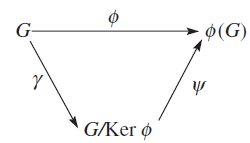
\includegraphics[width=0.35\linewidth]{figures/thm10.3.png}
           \caption{}
           \label{thm10.3}
       \end{figure}
    \end{note}
    
    \begin{example}
        Let $\phi:\mathbb{Z}\to Z_n, \phi(m)=m\bmod{n}$ be a homomorphism. Since $a\in\mathbb{Z}:\phi(a)=a\bmod{n}=0 \implies a\in\{0,n\}$, therefore $\Ker\phi=\langle n\rangle=\{0,n\}$. By Theorem 10.3, $\mathbb{Z}/\Ker\phi\approx\phi(\mathbb{Z})=Z_n$.
    \end{example}
    
    \begin{example}
        The warping function $W$ maps each $a\in\mathbb{R}$ to a point $a$ radian from (1,0) on the unit circle centered at (0,0). The positive reals in the counterclockwise direction, the negative reals in the clockwise direction, and $W(0)=(1,0)$ (Figure \ref{exp10.14}). $W$ is a homomorphism from $\mathbb{R}$ under addition onto the circle group , the group of complex number of magnitude 1 under multiplication. From elementary trigonometry facts,
        \begin{align*}
            W(x)&=\cos{x}+i\sin{x}, \\
            W(x+y)&=W(x)W(y).
        \end{align*}
        Since $W$ is periodic of period $2\pi$, therefore $\Ker W=\langle 2\pi\rangle$. So, from the First Isomorphism Theorem, $\mathbb{R}/\langle 2\pi\rangle \approx$ the circle group.
        
        \begin{figure}[!htbp]
            \centering
            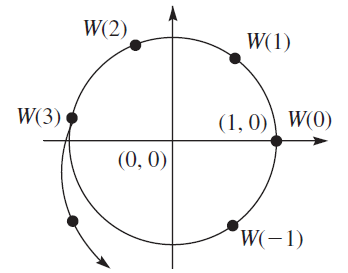
\includegraphics[width=0.35\linewidth]{figures/exp10.14.png}
            \caption{}
            \label{exp10.14}
        \end{figure}
    \end{example}
    
    \begin{example}
        Let $H\leq G$. The normalizer of $H$ in $G$ is $N(H)=\{x\in G: xHx^{-1}=H\}$ and the centralizer of $H$ in $G$ is $C(H)=\{x\in G: xhx^{-1}=h,h\in H\}$. Let $\psi:N(H)\to Aut(H),\psi(g)=\phi_g$, where $\phi_g(h)=ghg^{-1},h\in H$ is the inner automorphism of $H$ induced by $g$. The mapping $\psi$ is a homomorphism with $\Ker\psi=C(H)$. So, by the First Isomorphism Theorem,
        \begin{equation*}
            N(H)/\Ker\psi = N(H)/C(H) \approx \psi(N(H)) \leq Aut(H).
        \end{equation*}
    \end{example}
    
    \begin{example}
        Let $|G|=35$. By Lagrange's Theorem,
        \begin{equation*}
            g \in G, g\neq e, |g|=|\langle g\rangle| \mid |G| = 35.
        \end{equation*}
        Hence, $|g|\in\{5,7,35\}$. If $\exists a \in G:|a|=35$, then $G=\langle a\rangle$. So assume that $g\in G, a\neq e,|g|\in\{5,7\}$. But not all $g\in G$ can have order 5, since $g\in G:|g|=5$ come 4 at a time ($|x|=5\implies|x^2|=|x^3|=|x^4|=5$) and 4 does not divide 34. Similarly, since 6 does not divide 34, not all $g\in G$ can have order 7. Hence, $G$ has elements of order 5 and 7. Since $\exists g\in G:|g|=7$, $\exists H\leq G:|H|=7$. In fact, $H$ is the only subgroup of $G$ of order 7, since if $K\leq H,|K|=7$, then
        \begin{equation*}
            |HK|=|H||K|/|H \cap K|=7\cdot7/1=49.
        \end{equation*}
        But this is impossible in a group of order 35. Since $a\in G, aHa^{-1}\leq G,|aHa^{-1}|=7$, therefore $H=aHa^{-1}$.  So, $N(H)=G$. Since $H$ has prime order, it is cyclic and therefore Abelian. In particular, $C(H)$ contains $H$. So, $7\mid|C(H)|$ and $|C(H)|\mid35$. It follows that $C(H)=G$ or $C(H)=H$. If $C(H)=G$, then an element $x$ of order 35 can be obtained by letting $x=hk$, where $h\in H, h\neq e$ and $|k|=5$. If $C(H)=H$, then $|C(H)=7$ and $|N(H)/C(H)|=35/7=5$. However, 5 does not divide $|Aut(H)|=|Aut(Z_7)|=6$. This contradiction shows that $G$ is cyclic.
    \end{example}
    
    \noindent\fbox{\parbox{\linewidth}{
    \begin{theorem}[Normal Subgroups Are Kernels]
    Let $\phi:G\to\overline{G}$ be a homomorphism. Then
    \begin{equation*}
        H\lhd G \implies H=\Ker\phi.
    \end{equation*}
    In particular, let $\gamma:G\to G/N,\gamma(g)=gN$ be a homomorphism called the \textit{natural homomorphism} from $G$ to $G/N$. Then,
    \begin{equation*}
        N\lhd G \implies N=\Ker\gamma.
    \end{equation*}
    \end{theorem}
    }}
    
    \begin{proof}
       Let $\gamma:G\to G/N, \gamma(g)=gN$ be the natural homomorphism from $G$ to $G/N$. Then,
       \begin{equation*}
           \gamma(xy)=(xy)N=xNyN=\gamma(x)\gamma(y).
       \end{equation*}
       Moreover,
       \begin{equation*}
           g\in\Ker\gamma\iff gN=\gamma(g)=N.
       \end{equation*}
       By Lemma 7.1.2,
       \begin{equation*}
           gN=N\iff g\in N.
       \end{equation*}
       Hence,
       \begin{equation*}
           \Ker\gamma\subseteq N, N\subseteq\Ker\gamma \implies N=\Ker\gamma.
       \end{equation*}
    \end{proof}
    
    \section{Fundamental Theorem of Finite Abelian Groups}
    \subsection{The Fundamental Theorem}
    \fbox{\parbox{\linewidth}{
    \begin{theorem}[Fundamental Theorem of Finite Abelian Groups]
    Let $G$ be a finite Abelian group. Then
    \begin{equation*}
        G = H_1 \oplus H_2 \oplus \cdots \oplus H_k,
    \end{equation*}
    where $H_i$'s are cyclic groups of order prime-power, i.e. $|H_i|=p_i^{n_i}$. Moreover, the number of $H_i$ in the product and $|H_i|$ are uniquely determined by $G$.
    \end{theorem}
    }}
    
    \begin{note}
        Let $G$ be a finite Abelian group. Then by the Fundamental Theorem,
        \begin{equation*}
            G = H_1 \oplus H_2 \oplus \cdots \oplus H_k,
        \end{equation*}
        where $H_i$'s are cyclic and $|H_i|=p_i^{n_i}$. Since a cyclic group of order $n$ is isomorphic to $\mathbb{Z}_n$, therefore $H_i \approx \mathbb{Z}_{p_i^{n_i}}$. Hence,
       \begin{equation*}
           G \approx \mathbb{Z}_{p_1^{n_1}} \oplus \mathbb{Z}_{p_2^{n_2}} \oplus \cdots \oplus \mathbb{Z}_{p_k^{n_k}},
       \end{equation*}
       where $p_i$'s are not necessarily distinct primes and the prime-powers $p_1^{n_1},p_2^{n_2},\dots,p_k^{n_k}$ are uniquely determined by $G$. Writing a group in this form is called \textit{determining the isomorphism class of $G$}.
    \end{note}
    
    \subsection{The Isomorphism Classes of Abelian Groups}
    \begin{note}
        The Fundamental Theorem can be used as an algorithm to construct all Abelian groups of any order. Consider Abelian groups $G,|G|=p^k$, where $p$ is prime and $k \leq 4$. In general, there is one group of order $p^k$ for each set of positive integers whose sum is $k$ (such a set is called a \textit{partition of $k$}); that is, if
        \begin{equation*}
            k=n_1+n_2+\cdots n_t,
        \end{equation*}
        where $n_i$'s are positive integers, then
        \begin{equation*}
            \mathbb{Z}_{p^{n_1}} \oplus \mathbb{Z}_{p^{n_2}} \oplus \cdots \oplus \mathbb{Z}_{p^{n_t}}
        \end{equation*}
        is an Abelian group of order $p^k$ (Figure \ref{sec11.2}).
        
        \begin{figure}[!htbp]
            \centering
            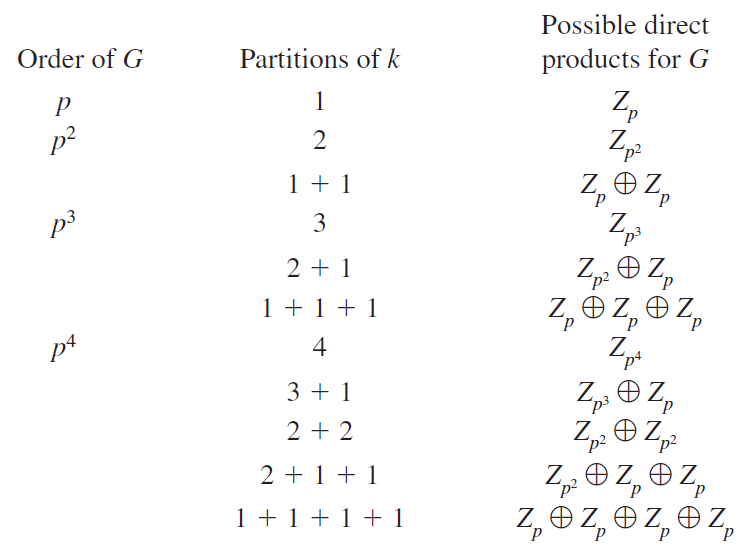
\includegraphics[width=0.75\linewidth]{figures/sec11.2.png}
            \caption{}
            \label{sec11.2}
        \end{figure}
        
        Furthermore, the uniqueness portion of the Fundamental Theorem guarantees that distinct partitions of $k$ yield distinct isomorphism classes. Thus, for example, $\mathbb{Z}_9 \oplus \mathbb{Z}_3$ is not isomorphic to $\mathbb{Z}_3 \oplus \mathbb{Z}_3 \oplus \mathbb{Z}_3$. A reliable mnemonic for comparing external direct products is the cancellation property. If $A$ is finite, then
        \begin{equation*}
            A \oplus B \approx A \oplus C \iff B \approx C.
        \end{equation*}
        Thus $\mathbb{Z}_4 \oplus \mathbb{Z}_4$ is not isomorphic to $\mathbb{Z}_4 \oplus \mathbb{Z}_2 \oplus \mathbb{Z}_2$ since $\mathbb{Z}_4$ is not isomorphic to $\mathbb{Z}_2 \oplus \mathbb{Z}_2$.
        
        Now that one knows how to construct all the Abelian groups of prime power order, the next step is to construct all Abelian groups of a certain order $n$, where $n$ has two or more distinct prime divisors. First, write $n$ in prime-power decomposition form
        \begin{equation*}
            n=p_1^{n_1}p_2^{n_2}\cdots p_k^{n_k}.
        \end{equation*}
        Next, individually form all Abelian groups of order $p_1^{n_1}$, then $p_2^{n_2}$, and so on, as described earlier. Finally, form all possible external direct products of these groups. For example, let $G$ be an Abelian group of order
        \begin{equation*}
            n=1176=2^3\cdot3\cdot7^2.
        \end{equation*}
        Then, for $2^3$, since
        \begin{align*}
            p=2,k&=3\\
            &=2+1\\
            &=1+1+1,
        \end{align*}
        the possible isomorphism classes for Abelian groups of order $2^3$ are
        \begin{align*}
            \mathbb{Z}_8 &,\\
            \mathbb{Z}_4 &\oplus\mathbb{Z}_2,\\
            \mathbb{Z}_2 &\oplus\mathbb{Z}_2\oplus\mathbb{Z}_2.
        \end{align*}
        For 3, since $p=3,k=1$, the only possible isomorphism class for Abelian groups of order 3 is $\mathbb{Z}_3$. For $7^2$, since
        \begin{align*}
            p=7,k=2=1+1,
        \end{align*}
        the possible isomorphism classes for Abelian groups of order $7^2$ are
        \begin{align*}
            \mathbb{Z}_{49}, \mathbb{Z}_7\oplus\mathbb{Z}_7.
        \end{align*}
        Hence, the complete list of the possible distinct isomorphism classes for $G$ is
        \begin{align*}
            \mathbb{Z}_8 &\oplus \mathbb{Z}_3 \oplus \mathbb{Z}_{49}, \\
            \mathbb{Z}_4 &\oplus \mathbb{Z}_2 \oplus \oplus \mathbb{Z}_3 \oplus \mathbb{Z}_{49}, \\
            \mathbb{Z}_2 &\oplus \mathbb{Z}_2 \oplus\mathbb{Z}_2\oplus\mathbb{Z}_3\oplus \mathbb{Z}_{49}, \\
            \mathbb{Z}_8 &\oplus \mathbb{Z}_3 \oplus\mathbb{Z}_7\oplus\mathbb{Z}_7, \\
            \mathbb{Z}_4 &\oplus \mathbb{Z}_2 \oplus \mathbb{Z}_3\oplus\mathbb{Z}_7\oplus\mathbb{Z}_7, \\
            \mathbb{Z}_2 &\oplus \mathbb{Z}_2 \oplus \mathbb{Z}_2\oplus\mathbb{Z}_3\oplus\mathbb{Z}_7\oplus\mathbb{Z}_7. \\
        \end{align*}
        
        To determine which of the preceding six isomorphism classes represents the structure of $G$, one can compare the orders of the elements of $G$ with the orders of the elements in the six direct products, since by Theorem 6.2.7, two finite Abelian groups are isomorphic if and only if they have the same number of elements of each order. For example, if $G$ has any elements of order 8, then $G$ must be isomorphic to the first or fourth group above, since these are the only groups with elements of order 8. Then, check if $G$ has any elements of order 49, since the first group above has elements of order 49, but the fourth group does not.
        
        Consider some specific Abelian group $G:|G|=p_1^{n_1}p_2^{n_2}\cdots p_k^{n_k}$, where $p_i$'s are distinct primes. One can express $G$ as an internal direct product of cyclic groups of prime-power order. For simplicity, assume that $G$ has $2^n$ elements. First, compute the orders of all the elements of $G$. Second, select a element $a_1\in G$ of maximum order $2^r$. Then $\langle a_1 \rangle$ is one of the factors in the desired internal direct product. If $G\neq\langle a_1 \rangle$, select an element $a_2\in G$ of maximum order $2^s$ such that
        \begin{equation*}
            s \leq n-r \text{ and } a_2,a_2^2,a_2^4,\dots,a_2^{2^{s-1}}\notin\langle a_1 \rangle.
        \end{equation*}
         Then $\langle a_2 \rangle$ is a second direct factor. If $n\neq r+s$, select an element $a_3\in G$ of maximum order $2^t$ such that $t\leq n-r-s$ and
         \begin{equation*}
            a_3,a_3^2,a_3^4,\dots,a_2^{2^{t-1}} \notin\langle a_1 \rangle \times \langle a_2 \rangle = \{a_1^ia_2^j: 0\leq i<2^r,0\leq j<2^s\}.
        \end{equation*}
        Then $\langle a_3 \rangle$ is another direct factor. Continue in this fashion until the internal direct product $\langle a_1\rangle\times\langle a_2\rangle\times\langle a_3\rangle\times\cdots$ has the same order as $G$.
        
        The greedy algorithm for an Abelian Group $G$ of order $p^n$ is as follows:
        \begin{enumerate}
            \item Compute the orders of all the elements of $G$.
            \item Select an $a_1\in G$ of maximum order and define $G_1=\langle a_1 \rangle$. Set $i=1$.
            \item If $|G|=|G_i|$, stop. Otherwise, replace $i$ by $i+1$.
            \item Select an $a_i\in G$ of maximum order $p^k$ such that $p^k\leq|G|/|G_{i-1}|$ and  $a_i,a_i^p,a_i^{p^2},\dots,a_i^{p^{k-1}}\notin G_{i-1}$, and define $G_i=G_{i-1}\times\langle a_i\rangle$.
            \item Return to step 3.
        \end{enumerate}
        
        In the general case where $|G|=p_1^{n_1}p_2^{n_2}\cdots p_k^{n_k}$, one simply use the algorithm to build up a direct product of order $p_1^{n_1}$, then another of order $p_2^{n_2}$, and so on. The direct product of all these pieces is the desired factorization of $G$.
    \end{note}
   
   \begin{example}
    Let $G=\{1,8,12,14,18,21,27,31,34,38,44,47,51,53,57,64\}$ under multiplication modulo 65. Since $|G|=16=2^4$,  the possible isomorphism classes for $G$ are
        \begin{align*}
           k&=4, & \mathbb{Z}_{16}&,\\
           &=3+1, & \mathbb{Z}_8&\oplus\mathbb{Z}_2,\\
           &=2+2, & \mathbb{Z}_4&\oplus\mathbb{Z}_4,\\
           &=2+1+1, & \mathbb{Z}_4&\oplus\mathbb{Z}_2\oplus\mathbb{Z}_2,\\
           &=1+1+1+1, & \mathbb{Z}_2&\oplus\mathbb{Z}_2\oplus\mathbb{Z}_2\oplus\mathbb{Z}_2.
        \end{align*}
        
    Figure \ref{exp11.1} shows the orders of the elements of $G$.
        
        \begin{figure}[!htbp]
            \centering
            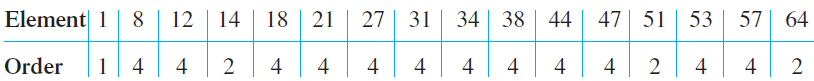
\includegraphics[width=0.95\linewidth]{figures/exp11.1.png}
            \caption{}
            \label{exp11.1}
        \end{figure}
        
        From Figure \ref{exp11.1}, since $G$ has no elements of order 16 and 8, and $G$ only has three elements of order 2, it must be that either
        \begin{equation*}
            G \approx \mathbb{Z}_4\oplus\mathbb{Z}_4 \text{ or } G \approx \mathbb{Z}_4\oplus\mathbb{Z}_2\oplus\mathbb{Z}_2.
        \end{equation*}
        Since $\mathbb{Z}_4\oplus\mathbb{Z}_2\oplus\mathbb{Z}_2$ has a subgroup isomorphic to $\mathbb{Z}_2\oplus\mathbb{Z}_2\oplus\mathbb{Z}_2$, it has more than three elements of order 2. Therefore, it must be that $G \approx \mathbb{Z}_4\oplus\mathbb{Z}_4$.
        
        To express $G$ as an internal direct product, select an element of maximum order, say $8\in G$. Then $\langle8\rangle$ is a factor in the product. Next select a second element $a\in G$ such that $|a|=4$ and 
        \begin{equation*}
            a,a^2\notin\langle8\rangle=\{1,8,64,57\}. 
        \end{equation*}
        Since 
        \begin{equation*}
            12\in G, |12|=4, \langle 12 \rangle = \{12, 14, 38, 1\}
        \end{equation*}
        it follows that $\langle12\rangle$ is the second factor in the product. Since
        \begin{equation*}
            |\langle8\rangle\times\langle12\rangle|=16=|G|,
        \end{equation*}
        it follows that $G=\langle8\rangle\times\langle12\rangle$.
   \end{example}
   
   \begin{example}
       Let 
       \begin{align*}
           G&=\{1,8,17,19,26,28,37,44,46,53,62,64, \\
           &71,73,82,89,91,98, 107, 109, 116, 118, 127, 134\}
       \end{align*}
        under multiplication modulo 135. Since $|G|=24=2^3\cdot3$, the possible isomorphism classes for Abelian groups of order $2^3$ are
       \begin{align*}
           k&=3, &\mathbb{Z}_8, \\
           &=2+1, &\mathbb{Z}_4&\oplus\mathbb{Z}_2, \\ &=1+1+1, &\mathbb{Z}_2&\oplus\mathbb{Z}_2\oplus\mathbb{Z}_2.
       \end{align*}
       The possible isomorphism class for Abelian groups of order 3 is $\mathbb{Z}_3$. Hence the possible isomorphism classes for $G$ are
       \begin{align*}
           \mathbb{Z}_8\oplus\mathbb{Z}_3&\approx\mathbb{Z}_{24},\\
           \mathbb{Z}_4\oplus\mathbb{Z}_2\oplus\mathbb{Z}_3&\approx\mathbb{Z}_{12}\oplus\mathbb{Z}_2,\\
           \mathbb{Z}_2\oplus\mathbb{Z}_2\oplus\mathbb{Z}_2\oplus\mathbb{Z}_3&\approx\mathbb{Z}_6\oplus\mathbb{Z}_2\oplus\mathbb{Z}_2.
       \end{align*}
       Consider $8\in G$. By direct calculations, $8^6=109$ and $8^{12}=1$. Since $|8|=12$, $G$ is not isomorphic to $\mathbb{Z}_6\oplus\mathbb{Z}_2\oplus\mathbb{Z}_2$. Since $|109|=2=|134|$, $G$ is not isomorphic to $\mathbb{Z}_{24}$. Hence $G\approx\mathbb{Z}_{12}\oplus\mathbb{Z}_2$, and $G=\langle8\rangle\times\langle134\rangle$.
   \end{example}
   
   \begin{note}
       Rather than express an Abelian group as a direct product of cyclic groups of prime-power orders, it is often more convenient to combine the cyclic factors of relatively prime order to obtain a direct product of the form
       \begin{equation*}
           \mathbb{Z}_{n_1}\oplus\mathbb{Z}_{n_2}\oplus\cdots\oplus\mathbb{Z}_{n_k}, n_i \mid n_{i-1},
       \end{equation*}
       like in Example 11.2. For example,
       \begin{equation*}
           \mathbb{Z}_4\oplus\mathbb{Z}_4\oplus\mathbb{Z}_2\oplus\mathbb{Z}_9\oplus\mathbb{Z}_3\oplus\mathbb{Z}_5
       \end{equation*}
       would be written as
       \begin{equation*}
           \mathbb{Z}_{180}\oplus\mathbb{Z}_{12}\oplus\mathbb{Z}_2.
       \end{equation*}
       The greedy algorithm is easily adapted to accomplish this by replacing step 4 by 4': select an element $a_i \in G$ of maximum order $m$ such that $m\leq|G|/|G_{i-1}|$ and $a_i,a_i^2,\dots,a_i^{m-1} \notin G_{i-1}$,
       and define $G_i=G_{i-1}\times\langle a_i \rangle$.
   \end{note}
    
    \noindent\fbox{\parbox{\linewidth}{
    \begin{corollary}
            Let $G$ be a finite Abelian group. Then,
            \begin{equation*}
                m \mid |G| \implies \exists H \leq G:|H|=m.
            \end{equation*}
    \end{corollary}
    }}
    
    \begin{note}
        Corollary 11.1.1 shows that the converse of Lagrange's Theorem is true for finite Abelian groups. Suppose $G$ is Abelian, $|G|=72$,  and one wishes to produce a $H \leq G, |H|=12$. By the Fundamental Theorem, since $|G|=72=2^33^2$, the possible isomorphism classes for Abelian groups of order $2^3$ and $3^2$ are
        \begin{align*}
            k&=3, & \mathbb{Z}_8, \\
            &=2+1, & \mathbb{Z}_4&\oplus\mathbb{Z}_2, \\ &=1+1+1, &\mathbb{Z}_2&\oplus\mathbb{Z}_2\oplus\mathbb{Z}_2.
        \end{align*}
        and
        \begin{align*}
            k&=2, & \mathbb{Z}_9, \\
            &=1+1, & \mathbb{Z}_3&\oplus\mathbb{Z}_3,
        \end{align*}
        respectively. Hence, $G$ is isomorphic to one of the following groups,
        \begin{align*}
            \mathbb{Z}_8&\oplus\mathbb{Z}_9, & \mathbb{Z}_8&\oplus\mathbb{Z}_3\oplus\mathbb{Z}_3, \\
            \mathbb{Z}_4&\oplus\mathbb{Z}_2\oplus\mathbb{Z}_9, & \mathbb{Z}_4&\oplus\mathbb{Z}_2\oplus\mathbb{Z}_3\oplus\mathbb{Z}_3, \\
            \mathbb{Z}_2&\oplus\mathbb{Z}_2\oplus\mathbb{Z}_2\oplus\mathbb{Z}_9, & \mathbb{Z}_2&\oplus\mathbb{Z}_2\oplus\mathbb{Z}_3\oplus\mathbb{Z}_3.
        \end{align*}
        By Corollary 11.1.1, since $12\mid72$, it follows that $\mathbb{Z}_8\oplus\mathbb{Z}_9\approx\mathbb{Z}_{72}$ and $\mathbb{Z}_4\oplus\mathbb{Z}_2\oplus\mathbb{Z}_3\oplus\mathbb{Z}_3\approx\mathbb{Z}_{12}\oplus\mathbb{Z}_6$ have a subgroup of order 12. To construct a subgroup of order 12 in $\mathbb{Z}_4\oplus\mathbb{Z}_2\oplus\mathbb{Z}_9$, one simply pieces together all of $\mathbb{Z}_4$ and the subgroup of order 3 in $\mathbb{Z}_9$; that is,
        \begin{equation*}
            \{(a,0,b):a\in\mathbb{Z}_4,b\in\{0,3,6\}\}.
        \end{equation*}
        An analogous procedure applies to the remaining cases and to any finite Abelian group.
    \end{note}
    
    \subsection{Proof of the Fundamental Theorem}
    \begin{note}
        The proof of the Fundamental Theorem is long and complex so it will be broke down into a series of lemmas.
    \end{note}
    
    \noindent\fbox{\parbox{\linewidth}{
    \begin{lemma}
        Let $G$ be a finite Abelian group, $|G|=p^nm$, where $p$ is a prime, $p\nmid m$. Then $G=H\times K$, where $H=\{x\in G: x^{p^n}=e\},K=\{x\in G: x^m=e\}$. Moreover, $|H|=p^n$.
    \end{lemma}
    }}
    
    \begin{proof}
       Let $G$ be a finite Abelian group, $|G|=p^nm$, where $p$ is a prime, $p\nmid m$. Let $H=\{x\in G: x^{p^n}=e\},K=\{x\in G: x^m=e\}$.
       
       By Definition 9.2,
       \begin{equation*}
           H,K \lhd G, G=HK, H\cap K=\{e\} \implies G=H\times K.
       \end{equation*} 
       By One-Step Subgroup Test,
       \begin{equation*}
           H \subseteq G, a,b\in H, ab^{-1} \in H \implies H \leq G.
       \end{equation*}
       Let $a,b\in H$ and $c,d\in K$. Then since $G$ is Abelian,
       \begin{align*}
           (ab^{-1})^{p^n} &= a^{p^n}(b^{-1})^{p^n} \\
           &= a^{p^n}(b^{p^n})^{-1} \\
           &= ee^{-1} \\
           &= e \\
           \therefore ab^{-1} &\in H,
       \end{align*}
       and
       \begin{align*}
           (cd^{-1})^m &= c^m(d^{-1})^m \\
           &= c^m(d^m)^{-1} \\
           &= ee^{-1} \\
           &= e \\
           \therefore cd^{-1} &\in K.
       \end{align*}
       Hence,
       \begin{equation*}
           ab^{-1}\in H, cd^{-1} \in K \implies H,K \leq G.
       \end{equation*}
       
      By Theorem 9.1,
      \begin{equation*}
          H \leq G, \forall x \in G, xHx^{-1} \subseteq G \implies H \lhd G.
      \end{equation*}
      Let $x\in G, h\in H, k\in K$. Let $xhx^{-1}\in xHx^{-1}, xkx^{-1}\in xKx^{-1}$, then
       \begin{align*}
           (xhx^{-1})^{p^n} &= x^{p^n}h^{p^n}(x^{-1})^{p^n} \\
           &=x^{p^n}h^{p^n}(x^{p^n})^{-1} \\
           &=  x^{p^n}e(x^{p^n})^{-1} \\
           &= x^{p^n}(x^{p^n})^{-1} \\
           &= e, \\
           \therefore xhx^{-1} &\in H \implies xHx^{-1} \subseteq H,
       \end{align*}
       and
       \begin{align*}
           (xkx^{-1})^m &= x^mk^m(x^{-1})^m \\
           &= x^mk^m(x^m)^{-1} \\
           &= x^me(x^m)^{-1} \\
           &= x^m(x^m)^{-1} \\
           &= e, \\
           \therefore xkx^{-1} &\in K \implies xKx^{-1} \subseteq K.
       \end{align*}
       Hence,
       \begin{equation*}
           H\lhd G, K\lhd G \iff \forall x\in G, xHx^{-1} \subseteq H, xKx^{-1} \subseteq K.
       \end{equation*}
       
       By Theorem 0.2,
       \begin{equation*}
           \forall a,b \in \mathbb{Z}, a\neq 0, b\neq 0, \exists s,t \in \mathbb{Z}: \gcd(a,b)=as+bt.
       \end{equation*}
       Since $p\nmid m$,
       \begin{equation*}
           \gcd(m,p^n)=1=sm+tp^n, s,t\in \mathbb{Z}.
       \end{equation*}
       Let $x\in G$. Then
       \begin{equation*}
           x=x^1=x^{sm+tp^n}=x^{sm}x^{tp^n}.
       \end{equation*}
       By Corollary 7.1.4,
       \begin{equation*}
           |G|=n,a\in G \implies a^{|G|}=e.
       \end{equation*}
       Since $|G|=p^nm,x\in G$, it follows that
       \begin{align*}
           x^s \in G \implies (x^{sm})^{p^n} &= (x^s)^{p^nm} = e, \\
           \therefore x^{sm} &\in H, \\
           x^k \in g \implies (x^{tp^n})^m &= (x^t)^{p^nm} = e, \\
           \therefore x^{tp^n} &\in K.
       \end{align*}
       Hence, $x\in HK \implies G \subseteq HK$. Let $hk \in HK, h\in H, k\in K$. Then
       \begin{equation*}
           h\in G, k\in G \implies hk \in G.
       \end{equation*}
       Hence, $HK \subseteq G$ and therefore $G=HK$.
       
       Let $x \in H \cap K$. By Corollary 4.1.2,
       \begin{equation*}
           a\in G, a^k=e \iff |a|\mid k.
       \end{equation*}
       Since $x \in H\cap K$, it follows that $x\in H, x\in K$ and
       \begin{equation*}
            x^{p^n}=e, x^m=e \iff |x| \mid p^n, |x|\mid m.
       \end{equation*}
       Since $1=sp^n+tm$, it follows that
       \begin{equation*}
           |x| \mid 1 \implies |x|=1.
       \end{equation*}
       Hence $x=e$ and $H\cap K=\{e\}$. Therefore, $G=H\times K$.
       
       By Theorem 7.2,
       \begin{equation*}
           H,K \leq G \implies |HK|=|H||K|/|H\cap K|.
       \end{equation*}
       Hence
       \begin{align*}
           p^nm=|G|&=|HK|\\
           &=|H||K|/|H\cap K|\\
           &=|H||K|/1\\
           &=|H||K|. 
       \end{align*}
       By Lemma 0.1,
       \begin{equation*}
           p\mid ab \implies p\mid a \text{ or } p\mid b.
       \end{equation*}
       It follows that 
       \begin{equation*}
           p\mid p^nm=|H||K| \implies p\mid |H| \text{ or } p\mid |K|.
       \end{equation*}
       If $p\mid|K|$, then by Theorem 9.5,
       \begin{equation*}
           p\mid|G|\implies \exists x\in G:|x|=p.
       \end{equation*}
       Hence
       \begin{equation*}
           p\mid|K| \implies \exists x \in K:|x|=p.
       \end{equation*}
       By Corollary 4.1.2,
       \begin{equation*}
           x \in K, x^m=e \iff |x|=p\mid m.
       \end{equation*}
       But $p \nmid m$. Hence $p\nmid|K|\implies p\mid |H|$. Therefore $|H|=p^n$.
    \end{proof}
    
    \begin{note}
        Given an Abelian group $G,|G|=p_1^{n_1}p_2^{n_2}\cdots p_k^{n_k}$, where $p_i$'s are distinct primes. Let $G(p_i)=\{x\in G: x^{p_i^{n_i}}=e\}$. Then by Lemma 11.1 and induction,
        \begin{equation*}
            G=G(p_1)\times G(p_2)\times\cdots\times G(p_k), |G(p_i)|=p_i^{n_i}.
        \end{equation*}
    \end{note}
    
    \noindent\fbox{\parbox{\linewidth}{
    \begin{lemma}
        Let $G$ be an Abelian group, $|G|=p^n$. Then
        \begin{equation*}
            a\in G \text{ is a maximal order element} \implies G=\langle a\rangle\times K, K \leq G.
        \end{equation*}
    \end{lemma}
    }}
    
    \begin{proof}
       Let $G$ be an Abelian group, $|G|=p^n$.
       
       By induction, let $n=1$, then $|G|=p$. Let $a\in G$ be a maximal order element. By Lagrange's Theorem,
       \begin{equation*}
           \langle a \rangle \leq G \implies |a|=|\langle a \rangle| \mid |G| = p.
       \end{equation*}
       Hence $|a|\in\{1,p\}$. Since by definition, $a$ is a maximal order element, therefore 
       \begin{equation*}
           |a|=p=|G| \implies G=\langle a \rangle=\langle a\rangle\times\langle e\rangle.
       \end{equation*}
       Hence the statement is true for $n=1$. Next, assume that the statement is true for $1\leq k<n$.
       
       Let $a\in G$ be the maximal order element, $|a|=p^m$. Then $\forall x \in G, |x|=p^s\mid p^m,1\leq s\leq m$. Therefore by Theorem 4.1.2,
       \begin{equation*}
           x^{p^m}=x^{p^s}=e \iff p^s\mid(p^m-p^s).
       \end{equation*}
       Hence $\forall x \in G, x^{p^m}=e$. If $G=\langle a\rangle$, then $G=\langle a \rangle \times \langle e \rangle, \langle e \rangle\leq G$. The proof is completed. If $G\neq\langle a\rangle$. Let $b\in G, b \notin \langle a\rangle$ be the smallest order element. By Theorem 4.2.2,
       \begin{equation*}
           |b^p|=|b|/\gcd(|b|,p)=|b|/p.
       \end{equation*}
       By the manner in which $b$ was chosen, it follows that $b^p \in \langle a \rangle$.
       (cont.)
    \end{proof}
    
    \noindent\fbox{\parbox{\linewidth}{
    \begin{lemma}
        Let $G$ be an Abelian group, $|G|=p^n$. Then 
        \begin{equation*}
            G=H_1\times H_2\times\cdots\times H_k,
        \end{equation*}
        where $H_i$'s are cyclic. 
    \end{lemma}
    }}
    
    \begin{note}
        By Lemma 11.1 and Note 11.6,
        \begin{equation*}
            G=G(p_1)\times G(p_2)\times\cdots\times G(p_k), |G(p_i)|=p_i^{n_i}.
        \end{equation*}
        By Lemma 11.3,
        \begin{equation*}
            G(p_i)=H_1 \times H_2 \times \cdots \times H_k,
        \end{equation*}
        where $H_i$'s are cyclic. Hence $G$ is an internal direct product of cyclic groups of prime order. Since 
        \begin{equation*}
            G(p_i)=\{x\in G: x^{p_i^{n_i}}=e\},
        \end{equation*}
        the groups $G(p_i)$ are uniquely determined by $G$.
    \end{note}
    
    \noindent\fbox{\parbox{\linewidth}{
    \begin{lemma}
        Let $G$ be an Abelian group, $|G|=p^n$. If
        \begin{align*}
            G=H_1\times H_2\times\cdots\times H_m \text{ and }
            G=K_1\times K_2\times\cdots\times K_n,
        \end{align*}
        where $H_i,K_i$ are nontrivial cyclic subgroups with
        \begin{align*}
            |H_1|\geq|H_2|\geq\cdots\geq|H_m| \text{ and }
            |K_1|\geq|K_2|\geq\cdots\geq|K_n|,
        \end{align*}
        then $m=n$ and $|H_i|=|K_i|$.
    \end{lemma}
    }}
    
    \begin{proof}
       
    \end{proof}
    
    \section{Introduction to Rings}
    \subsection{Motivation and Definition}
    \fbox{\parbox{\linewidth}{
    \begin{definition}[Ring]
        A \textit{ring} $R$ is a set with two binary operations, addition and multiplication, such that $\forall a,b,c \in R$:
        \begin{enumerate}
            \item $a+b=b+a$.
            \item $(a+b)+c = a+(b+c)$.
            \item There is an additive identity $0\in R: \forall a\in R, a+0=a$.
            \item $\forall a \in R, \exists-a \in R: a+(-a)=0$.
            \item a(bc)=(ab)c.
            \item $a(b+c)=ab+ac$ and $(b+c)a=ba+ca$.
        \end{enumerate}
    \end{definition}
    }}
    
    \begin{note}
        So, $R$ is an Abelian group under addition, also having an associative multiplication that is left and right distributive over addition. Note that multiplication need not be commutative. If $ab=ba$, then $R$ is \textit{commutative}. Also, $R$ need not have an identity under multiplication. If $e\in R, e\neq 0: \forall a \in R, ea=ae=a$, then $e$ is a \textit{unity} (or \textit{identity}). A nonzero element of a commutative ring with unity need not have a multiplicative inverse. When it does, it is a \textit{unit} of the ring. Thus, if $a^{-1}\in R$, then $a\in R$ is a unit.
        
        Let $a,b \in R, a\neq 0$, $R$ is commutative. If $\exists c \in R: b=ac$, then $a$ \textit{divides} $b$ (or $a$ is a \textit{factor} of $b$) and $a\mid b$. If $a$ does not divide $b$, then $a\nmid b$.
        
        Recall that if $a \in G$ under addition and $n \in \mathbb{Z}^+$, $na=a+a+\cdots+a$ ($n$ summands). When dealing with rings, this notation can cause confusion, since one also use juxtaposition for the ring multiplication. When there is the potential for confusion, one will use $n\cdot a = a+a+\cdots+a$ ($n$ summands).
    \end{note}
    
    \subsection{Examples of Rings}
    \begin{example}
        $\mathbb{Z}$ under addition and multiplication is a commutative ring with unity 1. The units of $\mathbb{Z}$ are 1 and -1.
    \end{example}
    
    \begin{example}
        $\mathbb{Z}_n=\{0,1,\dots,n-1\}$ under addition and multiplication modulo $n$ is a commutative ring with unity 1. The set of units is $U(n)$.
    \end{example}
    
    \begin{example}
        The set $\mathbb{Z}[x]$ of all polynomials in the variable $x$ with integer coefficients under addition and multiplication is a commutative ring with unity $f(x)=1$.
    \end{example}
    
    \begin{example}
        The set $M_2(\mathbb{Z})$ of $2\times2$ matrices with integers entries is a noncommutative ring with unity $I$.
    \end{example}
    
    \begin{example}
        The set $2\mathbb{Z}$ of even integers under addition and multiplication is a commutative ring without unity.
    \end{example}
    
    \begin{example}
        The set of all continuous real-valued functions of a real variable whose graphs pass through the point (1,0) is a commutative ring without unity under the operations of pointwise addition and multiplication, i.e. $f+g)(a)=f(a)+g(a)$ and $(fg)(a)=f(a)g(a)$.
    \end{example}
    
    \begin{example}
        Let $R_1,R_2,\dots,R_n$ be rings. These rings can be used to construct a new ring as follows. Let
        \begin{equation*}
            R_1\oplus R_2 \oplus\cdots\oplus R_n =\{(a_1,a_2,\dots,a_n):a_i\in R_i\}
        \end{equation*}
        and define
        \begin{equation*}
            (a_1,a_2,\dots,a_n)+(b_1,b_2,\dots,b_n)=(a_1+b_1,a_2+b_2,\dots,a_n+b_n)
        \end{equation*}
        and
        \begin{equation*}
            (a_1,a_2,\dots,a_n)(b_1,b_2,\dots,b_n)=(a_1b_1,a_2b_2,\dots,a_nb_n).
        \end{equation*}
        Then $ R_1\oplus R_2 \oplus\cdots\oplus R_n$ is a ring called the \textit{direct sum} of $R_1,R_2,\dots,R_n$.
    \end{example}
    
    
    \subsection{Properties of Rings}
    \begin{note}
        $b-c$ denotes $b+(-c)$.
    \end{note}
    
    \noindent\fbox{\parbox{\linewidth}{
    \begin{theorem}[Rules of Multiplication]
        Let $R$ be a ring, $a,b,c \in R$. Then
        \begin{enumerate}
            \item $a0=0a=0$.
            \item $a(-b)=(-a)b=-(ab)$.
            \item $(-a)(-b)=ab$.
            \item $a(b-c)=a(b+(-c))=ab-ac$ and $(b-c)a=(b+(-c))a=ba-ca$.
        \end{enumerate}
        Futhermore, if $R$ has a unity element 1, then
        \begin{enumerate}[resume]
            \item $(-1)a=-a$.
            \item $(-1)(-1)=1$.
        \end{enumerate}
    \end{theorem}
    }}
    
    \begin{proof}
        Let $R$ be a ring, $a,b,c \in R$.
        \begin{enumerate}
            \item By Definition 12.1.6,
            \begin{equation*}
                0+a0=a0=a(0+0)=a0+a0.
            \end{equation*}
            By cancellation,
            \begin{align*}
                0+a0+(-a0)&=a0+a0+(-a0) \\
                0&=a0.
            \end{align*}
            Similarly,
             \begin{align*}
                0+0a&=0a=(0+0)a=0a+0a \\
                0+0a+(-0a)&=0a+0a+(-0a) \\
                0&=0a.
            \end{align*}
            Hence, $a0=0a=0$.
            
            \item By Definition 12.1.6,
            \begin{align*}
                a(-b)+ab&=a(-b+b)=a0=0 \\
                a(-b)+ab+(-(ab))&=0+(-(ab)) \\
                a(-b)&=-(ab).
            \end{align*}
            Similarly,
            \begin{align*}
                (-a)b+ab&=(-a+a)b=0b=0 \\
                (-a)b+ab+(-(ab))&=0+(-(ab)) \\
                (-a)b&=-(ab).
            \end{align*}
            Hence, $a(-b)=(-a)b=-(ab)$.
            \item By Definition 12.1.6 and Theorem 12.1.1,
            \begin{align*}
                (-a)(-b)+(-ab)&=-a(-b+b)=-a0=0 \\
                (-a)(-b)+(-ab)+ab&=0+ab \\
                (-a)(-b)+(-a+a)b&=ab \\
                (-a)(-b)+(-a+a)b&=ab \\
                (-a)(-b)+0b&=ab \\
                (-a)(-b)+0&=ab \\
                \therefore (-a)(-b)&=ab.
            \end{align*}
            
            \item By Definition 12.1.6 and Theorem 12.1.2,
            \begin{align*}
                a(b-c)&=a(b+(-c)) \\
                &= ab+a(-c)\\
                &= ab-ac.
            \end{align*}
            Similarly,
            \begin{align*}
                (b-c)a&=(b+(-c))a\\
                &=ba+(-c)a\\
                &=ba-ca.
            \end{align*}
        \end{enumerate}
        
        Assume that $1\in R$, then
        \begin{enumerate}[resume]
            \item By Theorem 12.1.2, $(-1)a=-(1a)=-a$.
            
            \item By Theorem 12.1.3, $(-1)(-1)=(1)(1)=1$.
        \end{enumerate}
    \end{proof}
    
    \noindent\fbox{\parbox{\linewidth}{
    \begin{theorem}[Uniqueness of the Unity and Inverses]
        Let $R$ be a ring. Then
        \begin{enumerate}
            \item $R$ has a unity $\implies$ it is unique.
            \item $a\in R$, $a^{-1} \in R \implies a^{-1}\in R$ is unique.  
        \end{enumerate}
    \end{theorem}
    }}
    
    \begin{proof}
        Let $R$ be a ring.
        \begin{enumerate}
            \item Assume that $\exists e_1,e_2\in R:e_1a=ae_2=a$ and $e_2a=ae_2=a$. Then
            \begin{align*}
                e_1e_2=e_2e_1=e_1 \text{ and } e_2e_1=e_1e_2=e_2.
            \end{align*}
            Hence $e_1=e_2e_2=e_2e_1=e_2$.
            
            \item Assume that $a\in R, \exists a_1,a_2\in R: a_1a=aa_1=e$ and $a_2a=aa_2=e$. Then
            \begin{align*}
                a_1a&=a_2a & aa_1&=aa_2\\
                a_1aa_1&=a_2aa_1 & a_1aa_1&=a_1aa_2 \\
                a_1e&=a_2e & ea_1&=ea_2\\
                a_1&=a_2, & a_1&=a_2.
            \end{align*}
        \end{enumerate}
    \end{proof}
    
    \subsection{Subrings}
    \fbox{\parbox{\linewidth}{
    \begin{definition}[Subring]
        $S \subseteq R$ is a \textit{subring of} $R$ is a ring with the operations of $R$.
    \end{definition}
    }}
    
    \noindent\fbox{\parbox{\linewidth}{
    \begin{theorem}[Subring Test]
        Let $R$ be a ring, $S\subseteq R, S\neq \emptyset$. Then
        \begin{equation*}
            a,b \in S, a-b,ab \in S \implies S \text{ is a subring of } R.
        \end{equation*}
    \end{theorem}
    }}
    
    \begin{proof}
        Let $R$ be a ring, $S\subseteq R, S\neq \emptyset$. 
        
        Assume that $a,b \in S, a-b,ab \in S$. Since $R$ is a ring and $S \subseteq R$, by One-Step Subgroup test,
        \begin{equation*}
            a,b \in S, a-b\in S \implies S \leq R.
        \end{equation*}
        So $S$ is closed under addition, $0 \in S$, and $\forall a \in S, \exists -a \in S: a+(-a)=0$. Hence addition is a binary operation in $S$ and $S$ fulfills property 1 to 4 in Definition 12.1.
        
        Since $S \subseteq R$ and $a,b \in S, ab \in S$, it follows that multiplication is a binary operation in $S$ and $S$ fulfills property 5 and 6 of Theorem 12.1.
        
        Hence by Definition 12.1, $S$ is a subring of $R$.
    \end{proof}
    
    \begin{example}
        $\{0\}$ and $R$ are subrings of any ring $R$. 
        
        Since $\{0\}\subseteq R, \{0\}\neq\emptyset, 0-0,00 \in \{0\}$, by Theorem 12.3, $\{0\}$ is a subring of $R$.
        
        Since $R \subseteq R, 0 \in R \implies R \neq\emptyset, a,b \in R, a-b,ab \in R$, by Theorem 12.3, $R$ is a subring of $R$.
    \end{example}
    
    \begin{example}
        $\{0,2,4\}$ is a subring of the ring $\mathbb{Z}_6$. 
        
        Since $\{0,2,4\}\subseteq\mathbb{Z}_6,\{0,2,4\}$, and
        \begin{align*}
            0+0&=2+4=4+2=0, & 0(0)&=0(2)=0(4)=2(0)=4(0)=0, \\
            0+2&=2+0=4+4=2, & 2(2)&=4(4)=4,\\
            0+4&=2+2=4+0=4, & 2(4)&=4(2)=2,
        \end{align*}
        by Theorem 12.3, $\{0,2,4\}$ is a subgroup of $\mathbb{Z}_6$.
        
        Note that although 1 is the unity in $\mathbb{Z}_6$, 4 is the unity in $\{0,2,4\}$.
    \end{example}
    
    \begin{example}
        For each $n \in \mathbb{Z}^+$, the set
        \begin{equation*}
            n\mathbb{Z}=\{0,\pm n, \pm 2n, \pm 3n, \dots\}
        \end{equation*}
        is a subring of $\mathbb{Z}$.
        
        Since $n\mathbb{Z} \subseteq \mathbb{Z}, 0\in n\mathbb{Z} \implies n\mathbb{Z}\neq\emptyset$, and
        \begin{equation*}
            a,b \in n\mathbb{Z}, a-b,ab\in n\mathbb{Z},
        \end{equation*}
        By Theorem 12.3, $n\mathbb{Z}$ is a subring of $\mathbb{Z}$.
    \end{example}
    
    \begin{example}
        The set of Gaussian integers
        \begin{equation*}
            \mathbb{Z}[i]=\{a+bi:a,b\in\mathbb{Z}\}
        \end{equation*}
        is a substring of $\mathbb{C}$.
        
        Since $\mathbb{Z}[i] \subseteq\mathbb{C}, 0\in\mathbb{Z}[i]\implies\mathbb{Z}[i]\neq\emptyset$, and since $\mathbb{C},\mathbb{Z}$ are rings, $a+bi,c+di \in \mathbb{Z}[i]$,
        \begin{equation*}
             (a+bi)+(c+di)=(a+b)+(c+d)i \in \mathbb{Z}[i],
        \end{equation*}
        and
        \begin{align*}
            (a+bi)(c+di)&=(a+bi)c+(a+bi)(di) \\
            &= ac+bci+adi-bd \\
            &= (ac-bd)+(ad+bc)i\in\mathbb{Z}[i],
        \end{align*}
        by Theorem 12.3, $\mathbb{Z}[i]$ is a subring of $\mathbb{C}$.
    \end{example}
    
    \begin{example}
        Let $R$ be the ring of all real-valued functions of a single real variable under pointwise addition and multiplication. The subset $S\subseteq R$ of functions whose graphs pass through the origin forms a subring of $R$.
    \end{example}
    
    \begin{example}
        The set
        \begin{equation*}
        \bigg\{
            \begin{bmatrix}
               a & 0 \\ 0 & b
            \end{bmatrix}
            : a,b\in\mathbb{Z}\bigg\}
        \end{equation*}
        is a subring of the ring of all $2\times2$ matrices over $\mathbb{Z}$.
    \end{example}
    
    \begin{note}
        The relationship between a ring and its various subrings can be depicted as a subring lattice diagram (Figure \ref{subring-lattice-diagram}). In such a diagram, any ring is a subring of all the rings that it is connected to by one or more upward lines.
    \end{note}
    
    \begin{figure}[!htbp]
        \centering
        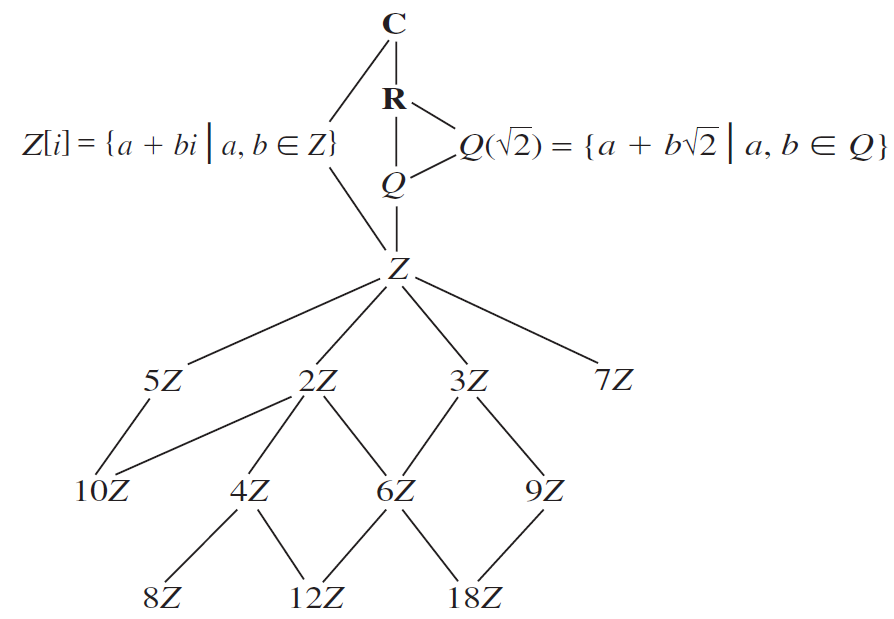
\includegraphics[width=0.7\linewidth]{figures/subring-lattice-diagram.png}
        \caption{}
        \label{subring-lattice-diagram}
    \end{figure}
    
\section{Integral Domains}
\subsection{Definition and Examples}
\fbox{\parbox{\linewidth}{
\begin{definition}[Zero-Devisors]
    Let $R$ be a commutative ring, $a\in R, a\neq 0$. Then
    \begin{equation*}
        \exists b \in R, b\neq0: ab=0 \implies a \text{ is a \textit{zero-divisor.}}
    \end{equation*}
\end{definition}
}}

\noindent\fbox{\parbox{\linewidth}{
\begin{definition}[Integral Domain]
    An \textit{integral domain} is a commutative ring with unity and no zero-divisors.
\end{definition}
}}

\begin{note}
    Thus, in an integral domain, a product is 0 only when one of the factor is 0; that is, $ab=0$ only when $a=0$ or $b=0$.
\end{note}

\begin{example}
    The ring of integers is an integral domain.
\end{example}

\begin{example}
    The ring of Gaussian integers $\mathbb{Z}[i]=\{a+bi:a,b\in\mathbb{Z}\}$ is an integral domain.
\end{example}

\begin{example}
    The ring $\mathbb{Z}[x]$ of polynomials with integer coefficients is an integral domain.
\end{example}

\begin{example}
    The ring $\mathbb{Z}[\sqrt{2}]=\{a+b\sqrt{2}:a,b\in\mathbb{Z}\}$ is an integral domain.
\end{example}

\begin{example}
    The ring $\mathbb{Z}_p$ of integers modulo a prime $p$ is an integral domain.
\end{example}

\begin{example}
    The ring $\mathbb{Z}_n$ of integers modulo $n$ is \textit{not} an integral domain when $n$ is not prime.
\end{example}

\begin{example}
    The ring $M_2(\mathbb{Z})$ of $2\times2$ matrices over the integers is \textit{not} an integral domain.
\end{example}

\begin{example}
    $\mathbb{Z}\oplus\mathbb{Z}$ is \textit{not} an integral domain.
\end{example}

\noindent\fbox{\parbox{\linewidth}{
\begin{theorem}[Cancellation]
    Let $R$ be an integral domain. Let $a,b,c \in R$. Then
    \begin{equation*}
        a\neq0, ab=ac \implies b=c.
    \end{equation*}
\end{theorem}
}}

\begin{proof}
    Let $R$ be an integral domain. Let $a,b,c \in R$. Assume that $a\neq0, ab=ac$. Then by Definition 12.1.6,
    \begin{align*}
        ab-ac&=a(b-c)=0.
    \end{align*}
    By Definition 13.2,
    since $R$ is an integral domain, 
    \begin{equation*}
        a(b-c)=0,a\neq0 \implies b-c=0.
    \end{equation*}
    Hence, $b-c=0\implies b=c$.
\end{proof}

\subsection{Fields}
\fbox{\parbox{\linewidth}{
\begin{definition}[Field]
    A \textit{field} is a commutative ring with unity in which every nonzero element is a unit.
\end{definition}
}}

\begin{note}
    To verify that every field is an integral domain, let $R$ be a field, observe that if $a,b\in R, a\neq0, ab=0$, then by Definition 13.3, $a\in R$ is a unit and hence $a^{-1}\in R$, so
    \begin{align*}
        ab&=0\\
        a^{-1}ab&=a^{-1}0\\
        \therefore b&=0.
    \end{align*}
    Hence by Definition 13.2, $R$ is a integral domain.
    
    It is often helpful to think of $ab^{-1}$ as $a$ divided by $b$. With this in mind, a field can be thought of as simply an algebraic system that is closed under addition, subtraction, multiplication, and division (except by 0). Some examples of fields are the complex numbers, the real numbers, the rational numbers.
\end{note}

\noindent\fbox{\parbox{\linewidth}{
\begin{theorem}[Finite Integral Domains Are Fields]
    A finite integral domain is a field.
\end{theorem}
}}

\begin{proof}
    Let $D$ be a finite integral domain. Let $a\in D, a\neq0$. If $a=1$, then $a(1)=1$. Since $1\in D$, it follows that $a^{-1}=1$ and $a$ is a unit.
    
    If $a\neq1$, then since $D$ is finite, the elements $a,a^2,a^3,\dots\in D$ are not all distinct. So 
    \begin{equation*}
        \exists i,j \in \mathbb{Z}, i>j: a^i=a^j.
    \end{equation*}
    Then by cancellation,
    \begin{align*}
        a^i&=a^j \\
        a^ia^{-j}&=a^ja^{-j} \\
        a^{i-j}&=1.
    \end{align*}
    Since $a\neq1$, it follows that
    \begin{equation*}
        i-j > 1 \implies i-j-1 > 0.
    \end{equation*}
    So 
    \begin{equation*}
        aa^{i-j-1}=a^{i-j}=1 \implies a^{-1}=a^{i-j} \in D
    \end{equation*}
    and $a$ is a unit. By Definition 13.3, $D$ is a field.
\end{proof}

\noindent\fbox{\parbox{\linewidth}{
\begin{corollary}[$\mathbb{Z}_p$ Is a Field]
    For every prime $p$, the ring of integers modulo $p$, $\mathbb{Z}_p$, is a field. 
\end{corollary}
}}

\begin{proof}
    Let $p$ be a prime and let  $\mathbb{Z}_p=\{0,1,2,\dots,p-1\}$ be a ring.
    Since $1\in\mathbb{Z}_p$ and $a,b\in\mathbb{Z}_p, ab=ba$, $\mathbb{Z}_p$ is a finite commutative ring with unity.
    
    Assume that $a,b\in\mathbb{Z}_p, a\neq0, ab=0$, then 
    \begin{equation*}
        ab=0 \implies ab=pk, k\in\mathbb{Z}.
    \end{equation*}
    Since $p\mid pk \implies p\mid ab$, so $p\mid a$ or $p\mid b$. If $p\mid a$, then $0\leq a<p\implies a=0$. If $p\mid b$, then $0\leq b<p\implies b=0$.
    
    Hence $\mathbb{Z}_p$ is a finite integral domain and by Theorem 13.2, $\mathbb{Z}_p$ is a field.
\end{proof}

\begin{example}[Field with Nine Elements]
    Let 
    \begin{align*}
        \mathbb{Z}_3[i]&=\{a+bi:a,b\in\mathbb{Z}_3\} \\
        &=\{0,1,2,i,1+i,2+i,2i,1+2i,2+2i\},
    \end{align*}
    where $i^2=-1$. This is the ring of Gaussian integers modulo 3. Elements are added and multiplied as in the complex numbers, except that the coefficients are reduced modulo 3. In particular, $-1=2$. Figure \ref{Z_3[i]-multiplication-table} shows the multiplication table for the nonzero elements of $\mathbb{Z}_3[i]$.
    
    \begin{figure}[!htbp]
        \centering
        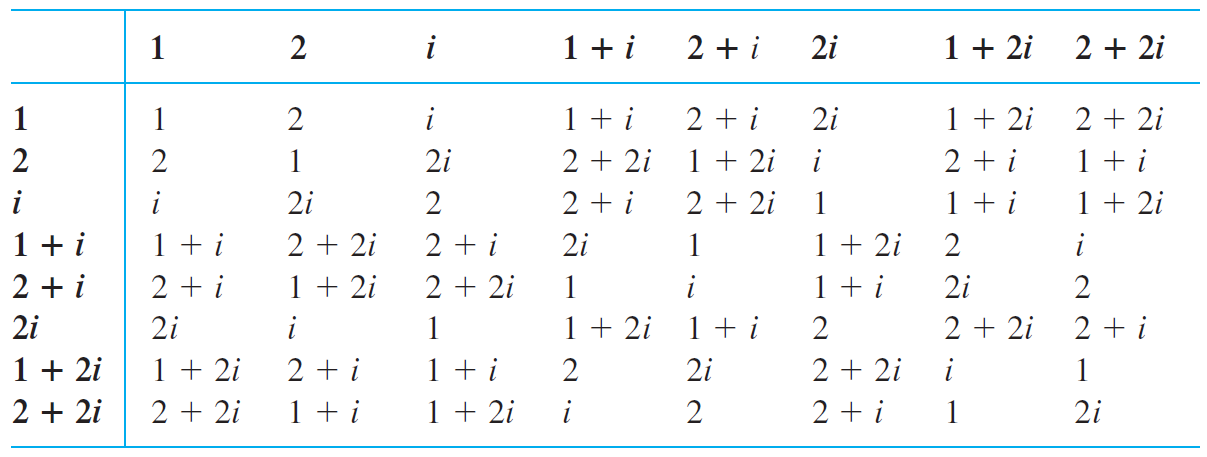
\includegraphics[width=0.9\linewidth]{figures/Z_3[i]-multiplication-table.png}
        \caption{Multiplication Table for $\mathbb{Z}_3[i]$.}
        \label{Z_3[i]-multiplication-table}
    \end{figure}
\end{example}

\begin{example}
    Consider the ring $\mathbb{Q}[\sqrt{2}]=\{a+b\sqrt{2}:a,b\in\mathbb{Q}\}$. The multiplicative inverse of any nonzero element of the form $a+b\sqrt{2}$ is $1/(a+b\sqrt{2})$. To verify that $\mathbb{Q[\sqrt{2}]}$ is a field, one must show that $1/(a+b\sqrt{2})$ can be written in the form $c+d\sqrt{2}$. This process is called "rationalizing the denominator". Specifically,
    \begin{equation*}
        \frac{1}{a+b\sqrt{2}}=\frac{1}{a+b\sqrt{2}}\frac{a-b\sqrt{2}}{a-b\sqrt{2}}=\frac{a}{a^2-2b^2}-\frac{b}{a^2-2b^2}\sqrt{2}.
    \end{equation*}
    Note that $a+b\sqrt{2}\neq0$ guarantees that $a-b\sqrt{2}\neq0$.
\end{example}

\subsection{Characteristic of a Ring}
\fbox{\parbox{\linewidth}{
\begin{definition}[Characteristic of a Ring]
    The \textit{characteristic} of a ring $R$, char $R=$ the least $n\in\mathbb{Z}^+:nx=0, \forall x \in R$. If no such integer exists, then char $R=0$.
\end{definition}
}}

\begin{note}
    Thus, char $\mathbb{Z}=0$, and char $\mathbb{Z}_n=n$. An infinite ring can have a nonzero characteristic. The ring $\mathbb{Z}_2[x]$ of all polynomials with coefficients in $\mathbb{Z}_2$ has characteristic 2 (Addition and multiplication are done as for polynomials with ordinary integer coefficients except that the coefficients are reduced modulo 2). 
\end{note}

\noindent\fbox{\parbox{\linewidth}{
\begin{theorem}[Characteristic of a Ring with Unity]
    Let $R$ be a ring with unity 1. Then
    \begin{enumerate}
        \item $|1|=\infty$ under addition $\implies$ char $R=0$.
        \item $|1|=n$ under addition $\implies$ char $R=n$.
    \end{enumerate}
\end{theorem}
}}

\begin{proof}
     Let $R$ be a ring with unity 1.
     \begin{enumerate}
         \item Assume that $|1|=\infty$ under addition. Then $1+1+\cdots\neq0$. Let $n\in\mathbb{Z}^+, x\in R$ be arbitrary and $nx=0$, then $x=k\cdot1$ and
         \begin{align*}
             nx&=0 \\
             n(k\cdot1)&=0 \\
             n(\underbrace{1+1+\cdots}_k)&=0 \implies n=0.
         \end{align*}
         Since $n$ is arbitrary, this is true for the least $n\in\mathbb{Z}^+$. Hence by Definition 13.4, char $R=0$.
         
         \item Assume that $|1|=n$ under addition. Then $n$ is the least positive integer s.t. $n\cdot1=0$. Let $x\in R$ be arbitrary, then
         \begin{align*}
             nx&=n(1\cdot x)=(n\cdot1)x=0x=0.
         \end{align*}
         Hence by Definition 13.4, char $R=n$.
     \end{enumerate}
\end{proof}

\noindent\fbox{\parbox{\linewidth}{
\begin{theorem}[Characteristic of an Integral Domain]
    Let $R$ be an integral domain. Then char $R=0$ or prime.
\end{theorem}
}}

\begin{proof}
     Let $R$ be an integral domain. Then by Theorem 13.3, if $|1|=\infty$, then char $R=0$. Let $|1|=n$, then char $R=n$. Since $1\in R, |1|=n$, it follows that $n\in R$. Hence 
     \begin{equation*}
         \exists s,t \in R: n=st, 1\leq s,t \leq n.
     \end{equation*}
     Then,
     \begin{equation*}
         0=n\cdot1=(st)\cdot1=(s\cdot1)(t\cdot1).
     \end{equation*}
     Since $R$ is an integral domain, it follows that $s\cdot1=0$ or $t\cdot1=0$. Since $n$ is the least positive integer s.t. $n\cdot1=0$, it follows that $s=n$ or $t=n$. Since $n=st$, it follows that $s,t\mid n$. If $s=n$, then $t=1$. If $t=n$, then $s=1$. So $n$ is only divisible by 1 and itself. Hence, $n$ is prime.
\end{proof}

\begin{figure}[!htbp]
    \centering
    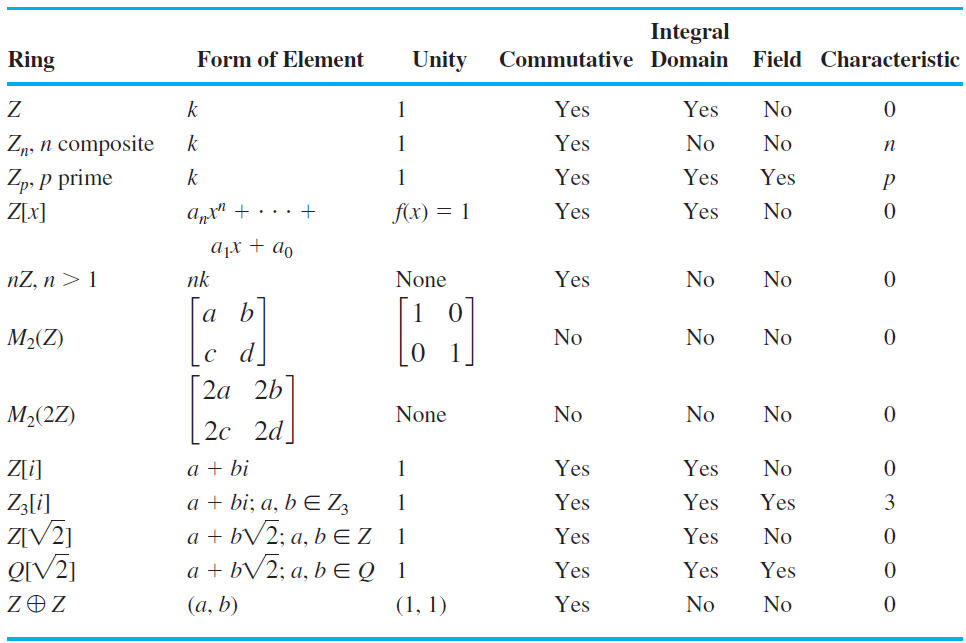
\includegraphics[width=\linewidth]{figures/ring-summary.png}
    \caption{Summary of rings and their properties.}
    \label{ring-summary}
\end{figure}
\end{document}